\documentclass[mathserif,handout]{beamer}
%\documentclass{beamer}
\usetheme{Warsaw}
\usecolortheme{seahorse}
\usecolortheme{orchid}
\usepackage{amsmath,verbatim}
\usepackage{listings}
\usepackage[english]{babel}
%\usepackage{movie15}
\setbeamercovered{transparent}

\newcommand{\Deltap}{\ensuremath{\Delta^{\!+}}}
\newcommand{\trans}{\ensuremath{{}^\mathrm{T}}}
\newcommand{\eps}{\varepsilon}
\newcommand*{\approxdist}{\mathrel{\vcenter{\offinterlineskip
\vskip-.25ex\hbox{\hskip.55ex$\cdot$}\vskip-.25ex\hbox{$\sim$}
\vskip-.5ex\hbox{\hskip.55ex$\cdot$}}}}

% \lstMakeShortInline[language=myR]¬

\lstdefinelanguage{myR}
{
   language=R,
   otherkeywords={read.table, set.seed, head},
   deletekeywords={url,codes, t, dt, Call, formula,Q, R, on,by,hat,is,
col, set,start,end,deltat,zip},
   sensitive=true,
   breaklines=true,
   morecomment=[l]{\#},
   morestring=[b]",
   morestring=[b]',
   basicstyle =\ttfamily\small,
   keywordstyle=\bfseries,
   showtabs=false,
   showstringspaces=false,
   literate= {~}{$\sim$}{2},
   numberstyle=\sffamily\scriptsize,
   stepnumber=2
 }



\title[Stochastic modelling of genetic interaction networks in yeast]{Stochastic Modelling of Genetic Interaction Networks in Budding Yeast}
\author[Darren Wilkinson --- RSS EAS, London, 8/5/2017]{\textbf{\large Darren 
Wilkinson} \\
\url{@darrenjw}\\
\alert{\url{tinyurl.com/darrenjw}}\\
School of Mathematics \& Statistics, \\
Newcastle University, UK}
\date{RSS EAS meeting on Statistical Network Science\\RSS, Errol Street, London\\8th May, 2017}

\begin{document}

\frame{\titlepage}


\frame{
\frametitle{Overview}
\begin{itemize}
%\item Background: Budding yeast as a model for genetics
\item High-throughput robotic genetic experiments
\item Image analysis and data processing
\item Stochastic modelling of growth curves
\item Hierarchical modelling of genetic interaction
\item Bayesian inference for a network of genetic interactions
%\item Functional approaches to scalable Bayesian modelling
%\item Potential CDT PhD project
%\item ``Big data'' challenges, summary and conclusions
\end{itemize}

Joint work with \alert{Jonathan Heydari}, \alert{Keith Newman}, \alert{Conor Lawless} and \alert{David Lydall} (and
others in the ``Lydall lab'')
\bigskip

Major funders: \alert{BBSRC}, \alert{MRC}, \alert{Wellcome Trust}, \alert{CRUK}

}



\section{Yeast}

\subsection{Budding yeast biology and genetics}

\frame{
\frametitle{Saccharomyces cerevisiae}
\begin{itemize}
\item \emph{Saccharomyces cerevisiae}, often known as budding yeast,
and sometimes as brewer's yeast or baker's yeast, is a single-celled
\alert{eukaryotic} organism
\item Eukaryotic cells contain a nucleus (and typically other
organelles, such as mitochondria)
%\item Budding yeast is an interesting species commercially, due to its use in
%baking, beer brewing, wine making, yeast extract, etc.
\item It is useful as a model for higher eukaryotes, having a
great deal of biological function \alert{conserved with humans}
\item It is the most heavily studied and well-characterised
model organism in biology (eg. first fully sequenced eukaryote)
\end{itemize}
}

\begin{comment}
  
\frame{
\frametitle{Budding yeast under the microscope}
\centerline{\includegraphics[height=0.9\textheight]{figs/S_cerevisiae_under_DIC_microscopy}}
}

\end{comment}

\subsection{Synthetic genetic array}

\frame{
\frametitle{Synthetic Genetic Array (SGA)}
\begin{itemize}
\item Possible to obtain a \alert{library} of around 4,500 
%MATa (haploid) 
mutant strains, each of which has one of the non-essential genes 
silenced through insertion of a (kanMX) antibiotic resistance 
cassette and tagged with a unique DNA barcode
\item These strains (stored frozen in 96-well plates) can be
manipulated by robots in 96-well plates (8$\times$12), or on solid
agar in 96, 384 or 1536-spot format
\item \alert{Synthetic Genetic Array} (SGA) is a clever genetic procedure
using robots to systematically introduce an additional mutation into
each strain in the library by starting from a specially constructed
%MAT$\alpha$ 
\alert{query strain} containing the new mutation
\end{itemize}
}


\subsection{Telomeres}

\frame{
\frametitle{Telomeres}
\begin{itemize}
\item The ends of linear chromosomes require special protection in
order not to be targeted by DNA damage repair machinery (bacteria
often avoid this problem by having just one chromosome arranged in a
single loop)
%\item The 2009 Nobel Prize for Physiology and Medicine was awarded to
%the discoverers of telomeres and telomerase...
\item \alert{Telomeres} are the ends of the chromosomal DNA (which have a
special sequence), bound with special telomere-capping proteins that
protect the telomeres
\item \alert{CDC13} is an essential \alert{telomere-capping protein} in yeast
\item \emph{cdc13-1} is a point-mutation of
\emph{cdc13}, encoding a \alert{temperature-sensitive} protein which functions similarly to
wild-type CDC13 below around $25\,^{\circ}\mathrm{C}$, and leads to
``telomere-uncapping'' above this temperature
\end{itemize}
}

\begin{comment}
  
\frame{
\frametitle{Telomeres, ageing and cancer}

Telomere function is critically important to human health,
affecting ageing, cancer, and other diseases. The main
function of telomeres is to stop the ends of chromosomes
initiating the \alert{DNA Damage Response} (DDR), which normally
responds to intra-chromosomal lesions such as \alert{Double Strand
Breaks} (DSBs). In most human somatic cells insufficient
telomerase is expressed to maintain telomere length and
with continuing cell division. Short
telomeres stimulate \alert{cell cycle arrest} (senescence) or
apoptosis and these processes contribute to \alert{ageing}. Another
consequence of telomere failure is \alert{genetic instability} and
\alert{cancer}, induced when telomeres are ``repaired" as if they were
intra-chromosomal DSBs leading to chromosome fusions and
breakage fusion bridge cycles.

}

\end{comment}

\section{Experiments}

\subsection{Lydall lab}

\frame{
\frametitle{Yeast Lab}
\begin{itemize}
\item \alert{David Lydall}'s (budding) yeast lab uses a range of high throughput (HTP) technologies for \alert{genome-wide screening} for
interactions relevant to DNA damage response and repair pathways, with
a particular emphasis on telomere maintenance
\item Much of this work centres around the use of \alert{robotic protocols}
in conjunction with genome-wide knockout libraries and \alert{synthetic
genetic array} (SGA) technology to screen for
\alert{genetic interactions} with known telomere maintenance genes 
\item \alert{Quantitative fitness analysis} (QFA) is the term we use for our
  system of robotic image capture, data handling, image analysis and
  data modelling
%(another talk...)
%\item The Lydall lab also utilises microarrays for studying cellular
%responses at the RNA level
%\item Time course HTP data is most useful for making inferences about
%dynamics
%\item \alert{Time course microarray data} is a typical example
\end{itemize}
}


\subsection{HTP yeast SGA robotic screens}

\frame{
\frametitle{Basic structure of an experiment}
\begin{enumerate}
\item Introduce a \alert{mutation} (such as
\emph{cdc13-1}) into an SGA query strain, and then use SGA technology
(and a robot) to \alert{cross} this strain with the single deletion library in
order to obtain a new library of double mutants
\item \alert{Inoculate} the strains into liquid media, grow up to saturation
then spot back on to solid agar 4 times
\item \alert{Incubate} the 4 different copies at different temperatures
(treatments), and image the plates multiple times to see how quickly
the different strains are growing
\item Repeat steps 2 and 3 four times (to get some idea of experimental
variation)
%\item Repeat steps 1 to 4 using a different version of the library
%which has the strains arranged differently on the plates (to
%ameliorate spatial location effects)
\item Repeat steps 2 to 4 with a ``control'' library that does not
  include the query mutation
\end{enumerate}
}

\frame{
\frametitle{Some numbers relating to an experiment}
\begin{itemize}
\item Initial SGA work (introducing mutations into the query and the
library) takes around \alert{1 month} of calendar time, and several days of
robot time
\item The inoculation, spotting and imaging of the 8 repeats takes
  \alert{1 month} of calendar time, and around 2 weeks of robot time
\item The experiment uses around \alert{\pounds 3,000} of consumables
(plastics and media) 
\item The library is distributed across 72 96-well plates or 18 solid agar
plates (in 384 format, or 1536 in quadruplicate)
\item If each plate is imaged 30 times, there will be around 35k
high-resolution photographs of plates in 384 format, corresponding to
around \alert{13 million} colony growth measurements (400k time
series)
\item This is \alert{big data}!
\end{itemize}
}



\frame{
\frametitle{HTP SGA robotic facility}
\centerline{
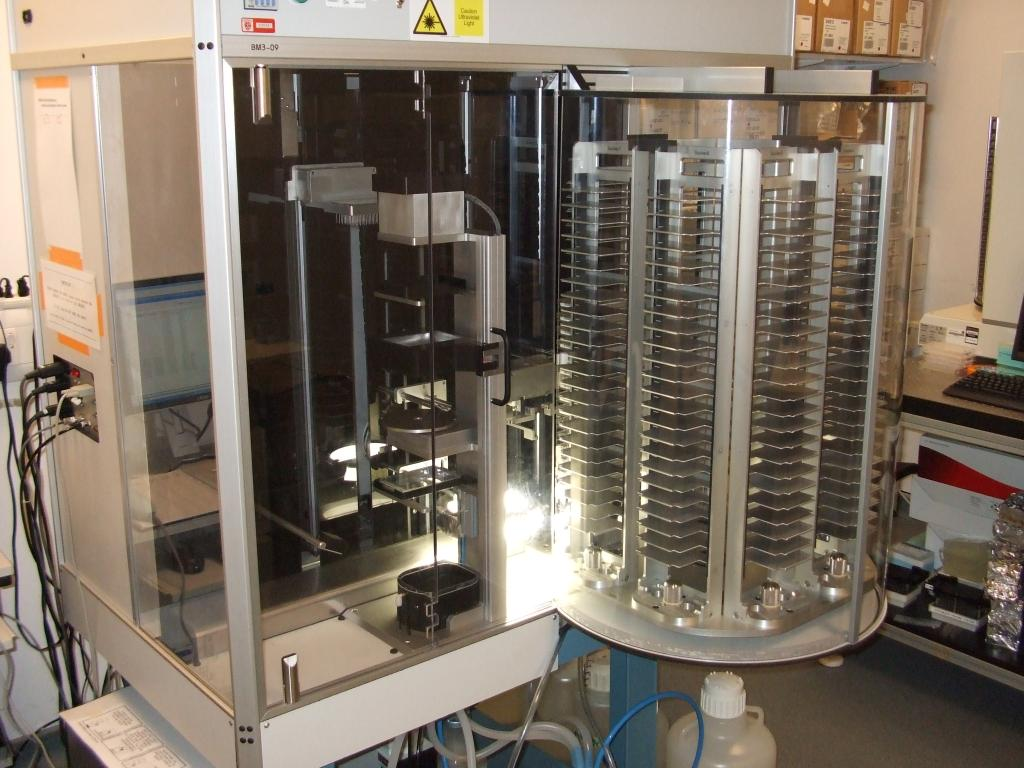
\includegraphics[height=0.4\textheight]{figs/robots-sticky}~
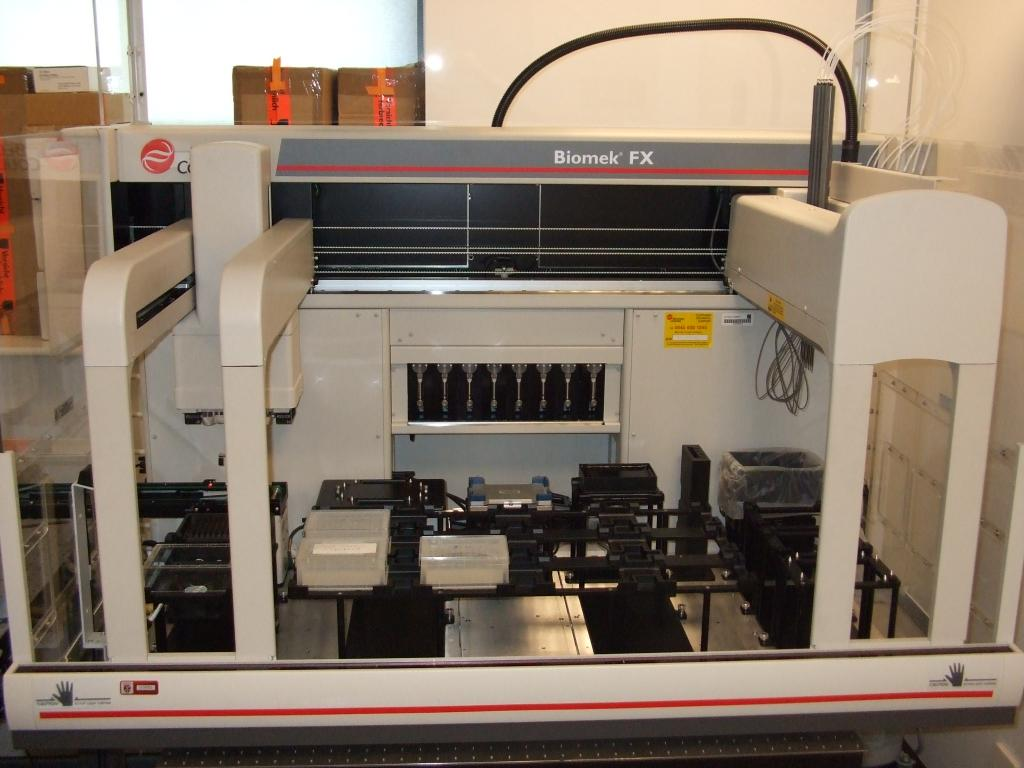
\includegraphics[height=0.4\textheight]{figs/robots-runny}~
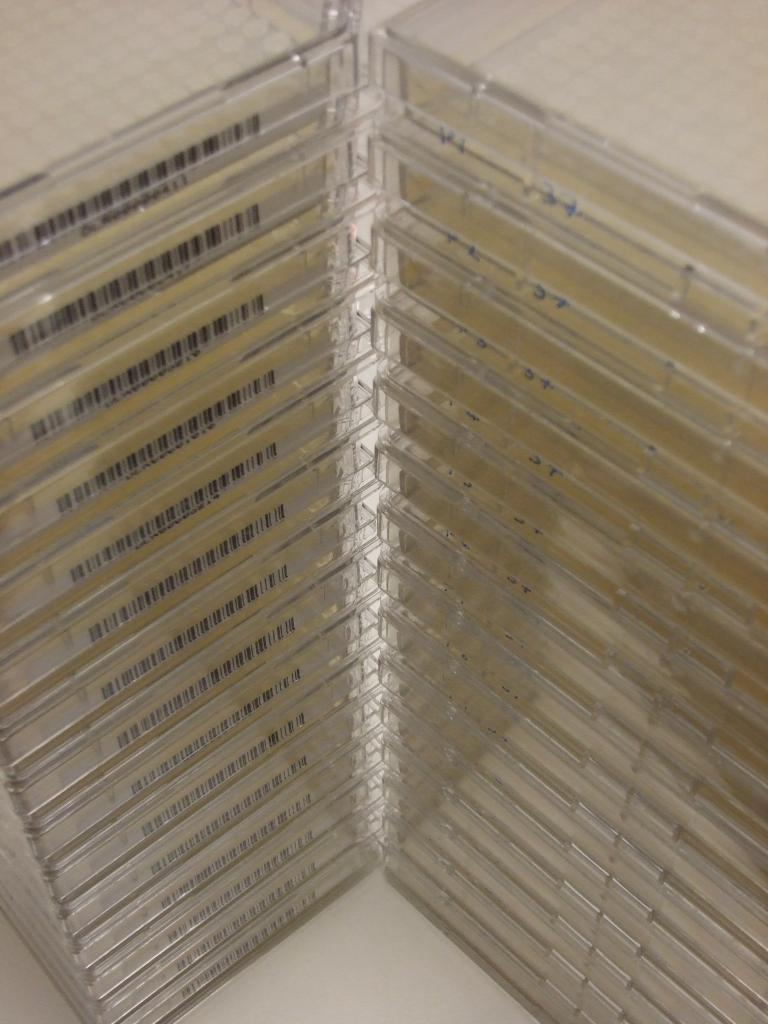
\includegraphics[height=0.4\textheight]{figs/robots-plates}
}
\vspace{0.5ex}
\centerline{
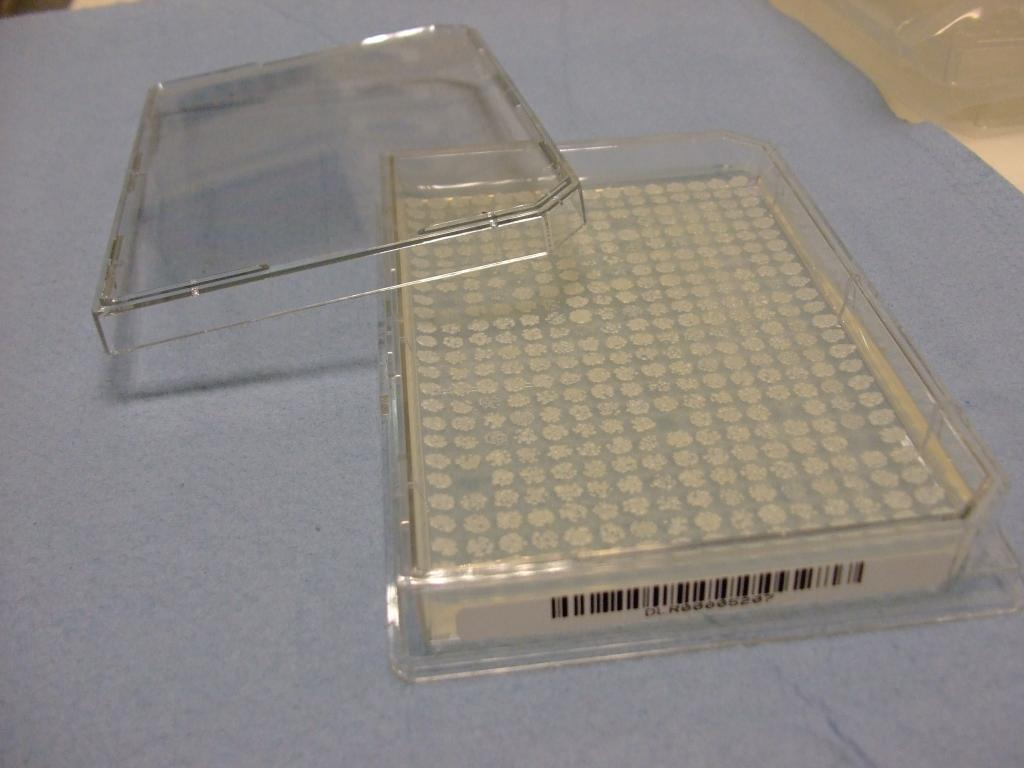
\includegraphics[height=0.4\textheight]{figs/robots-plate}~
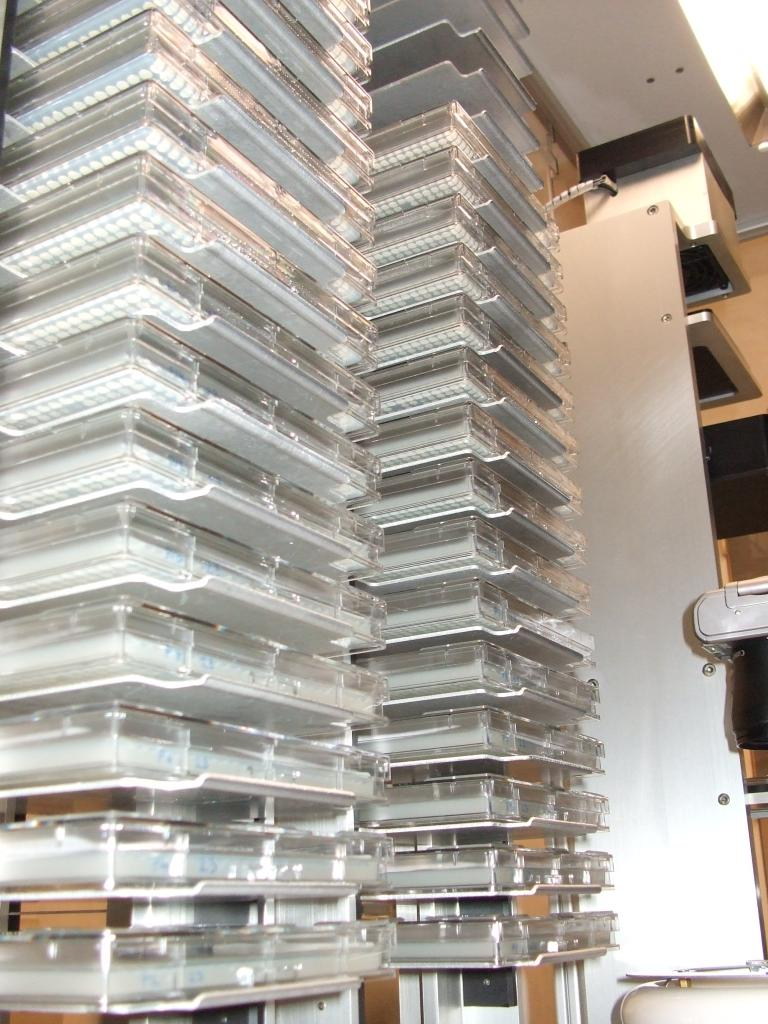
\includegraphics[height=0.4\textheight]{figs/robots-plates-sticky}~
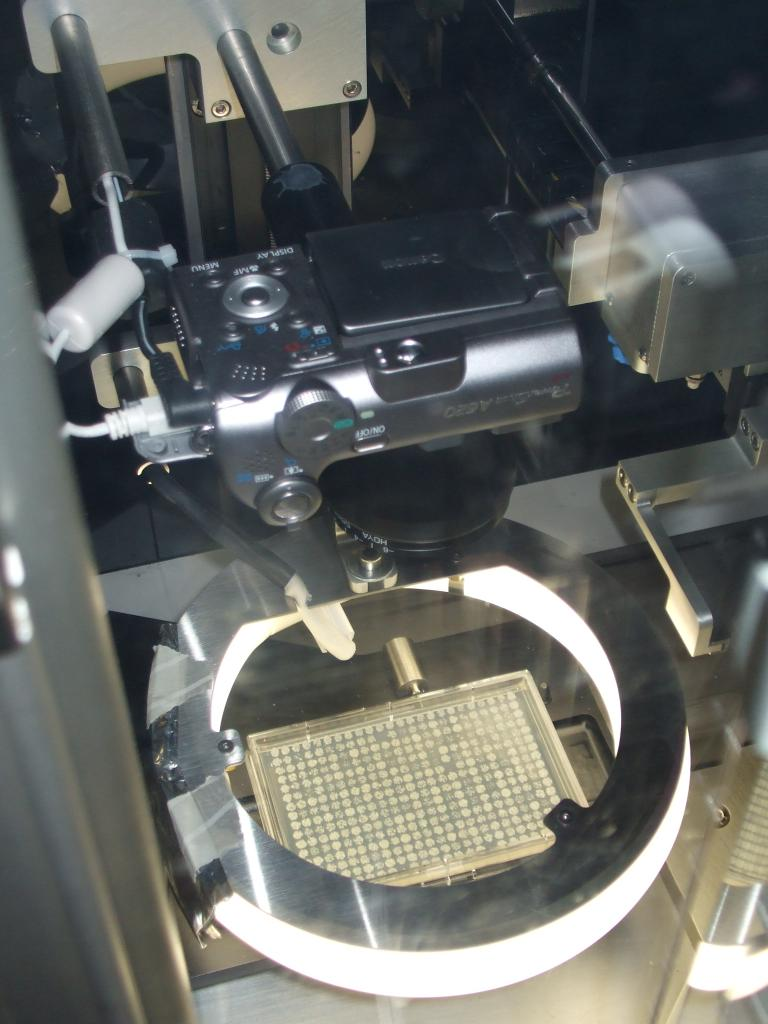
\includegraphics[height=0.4\textheight]{figs/robots-plate-photo}
}
}

\begin{comment}

\frame{
\frametitle{The colony handling robot}
\centerline{\includemovie[poster,text={Loading
movie...}]{0.8\textwidth}{0.8\textheight}{figs/robot.mpg}}
}

\end{comment}


\section{Data analysis}

\subsection{Data analysis pipeline}


\frame{
\frametitle{Data analysis pipeline}
\begin{itemize}
\item \alert{Image processing} (from images to colony size
  measurements)
\item \alert{Fitness modelling} (from colony size growth curves to
  strain fitness measures)
\item \alert{Modelling genetic interaction} (from strain fitness
  measures to identification of genetically interacting strains, ranked
  by effect size)
\end{itemize}
Possible to carry out three stages separately, but benefits to joint
modelling through borrowed strength and proper propagation of
uncertainty. Not practical to integrate image processing step into the
joint model, but possible to jointly model second two stages.
}


%\subsection{Image analysis}

\frame{
\frametitle{Automated image analysis (Colonyzer)}
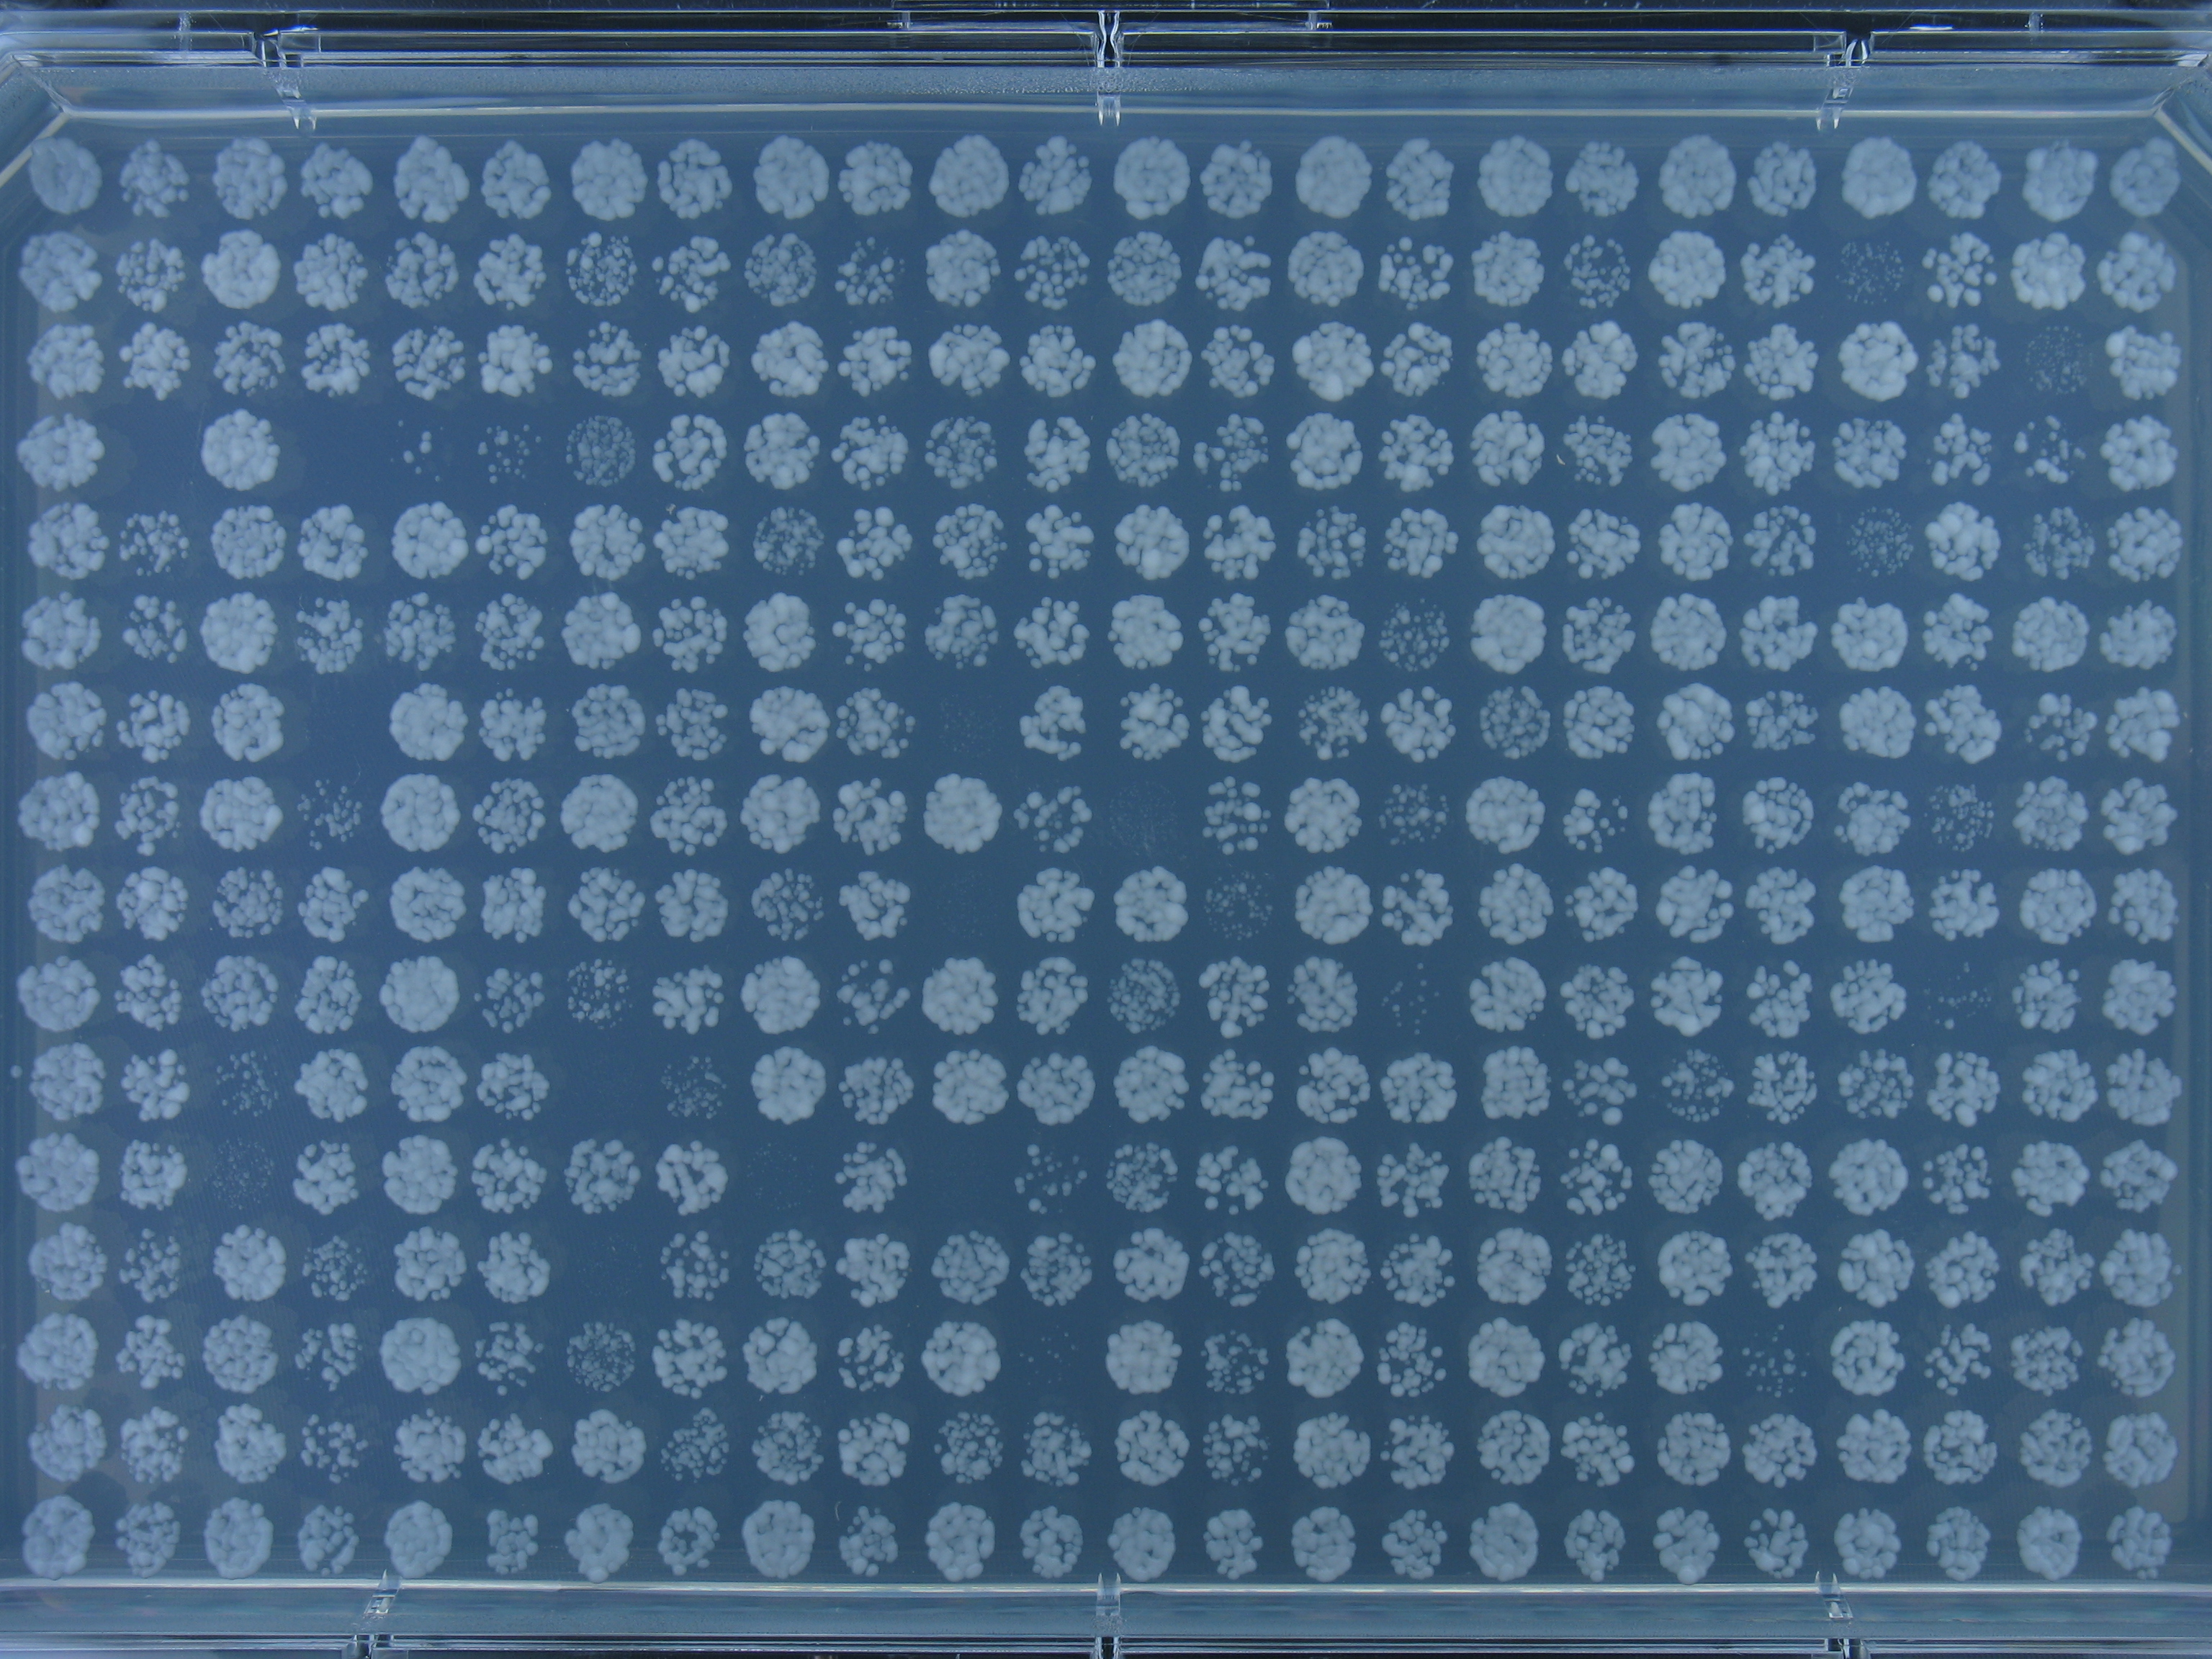
\includegraphics[height=0.4\textheight]{figs/rod-plate}\hspace{3ex}
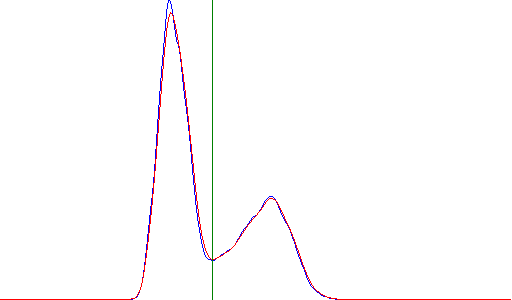
\includegraphics[height=0.4\textheight]{figs/rod-plate-hist}
\vspace{1ex}\\
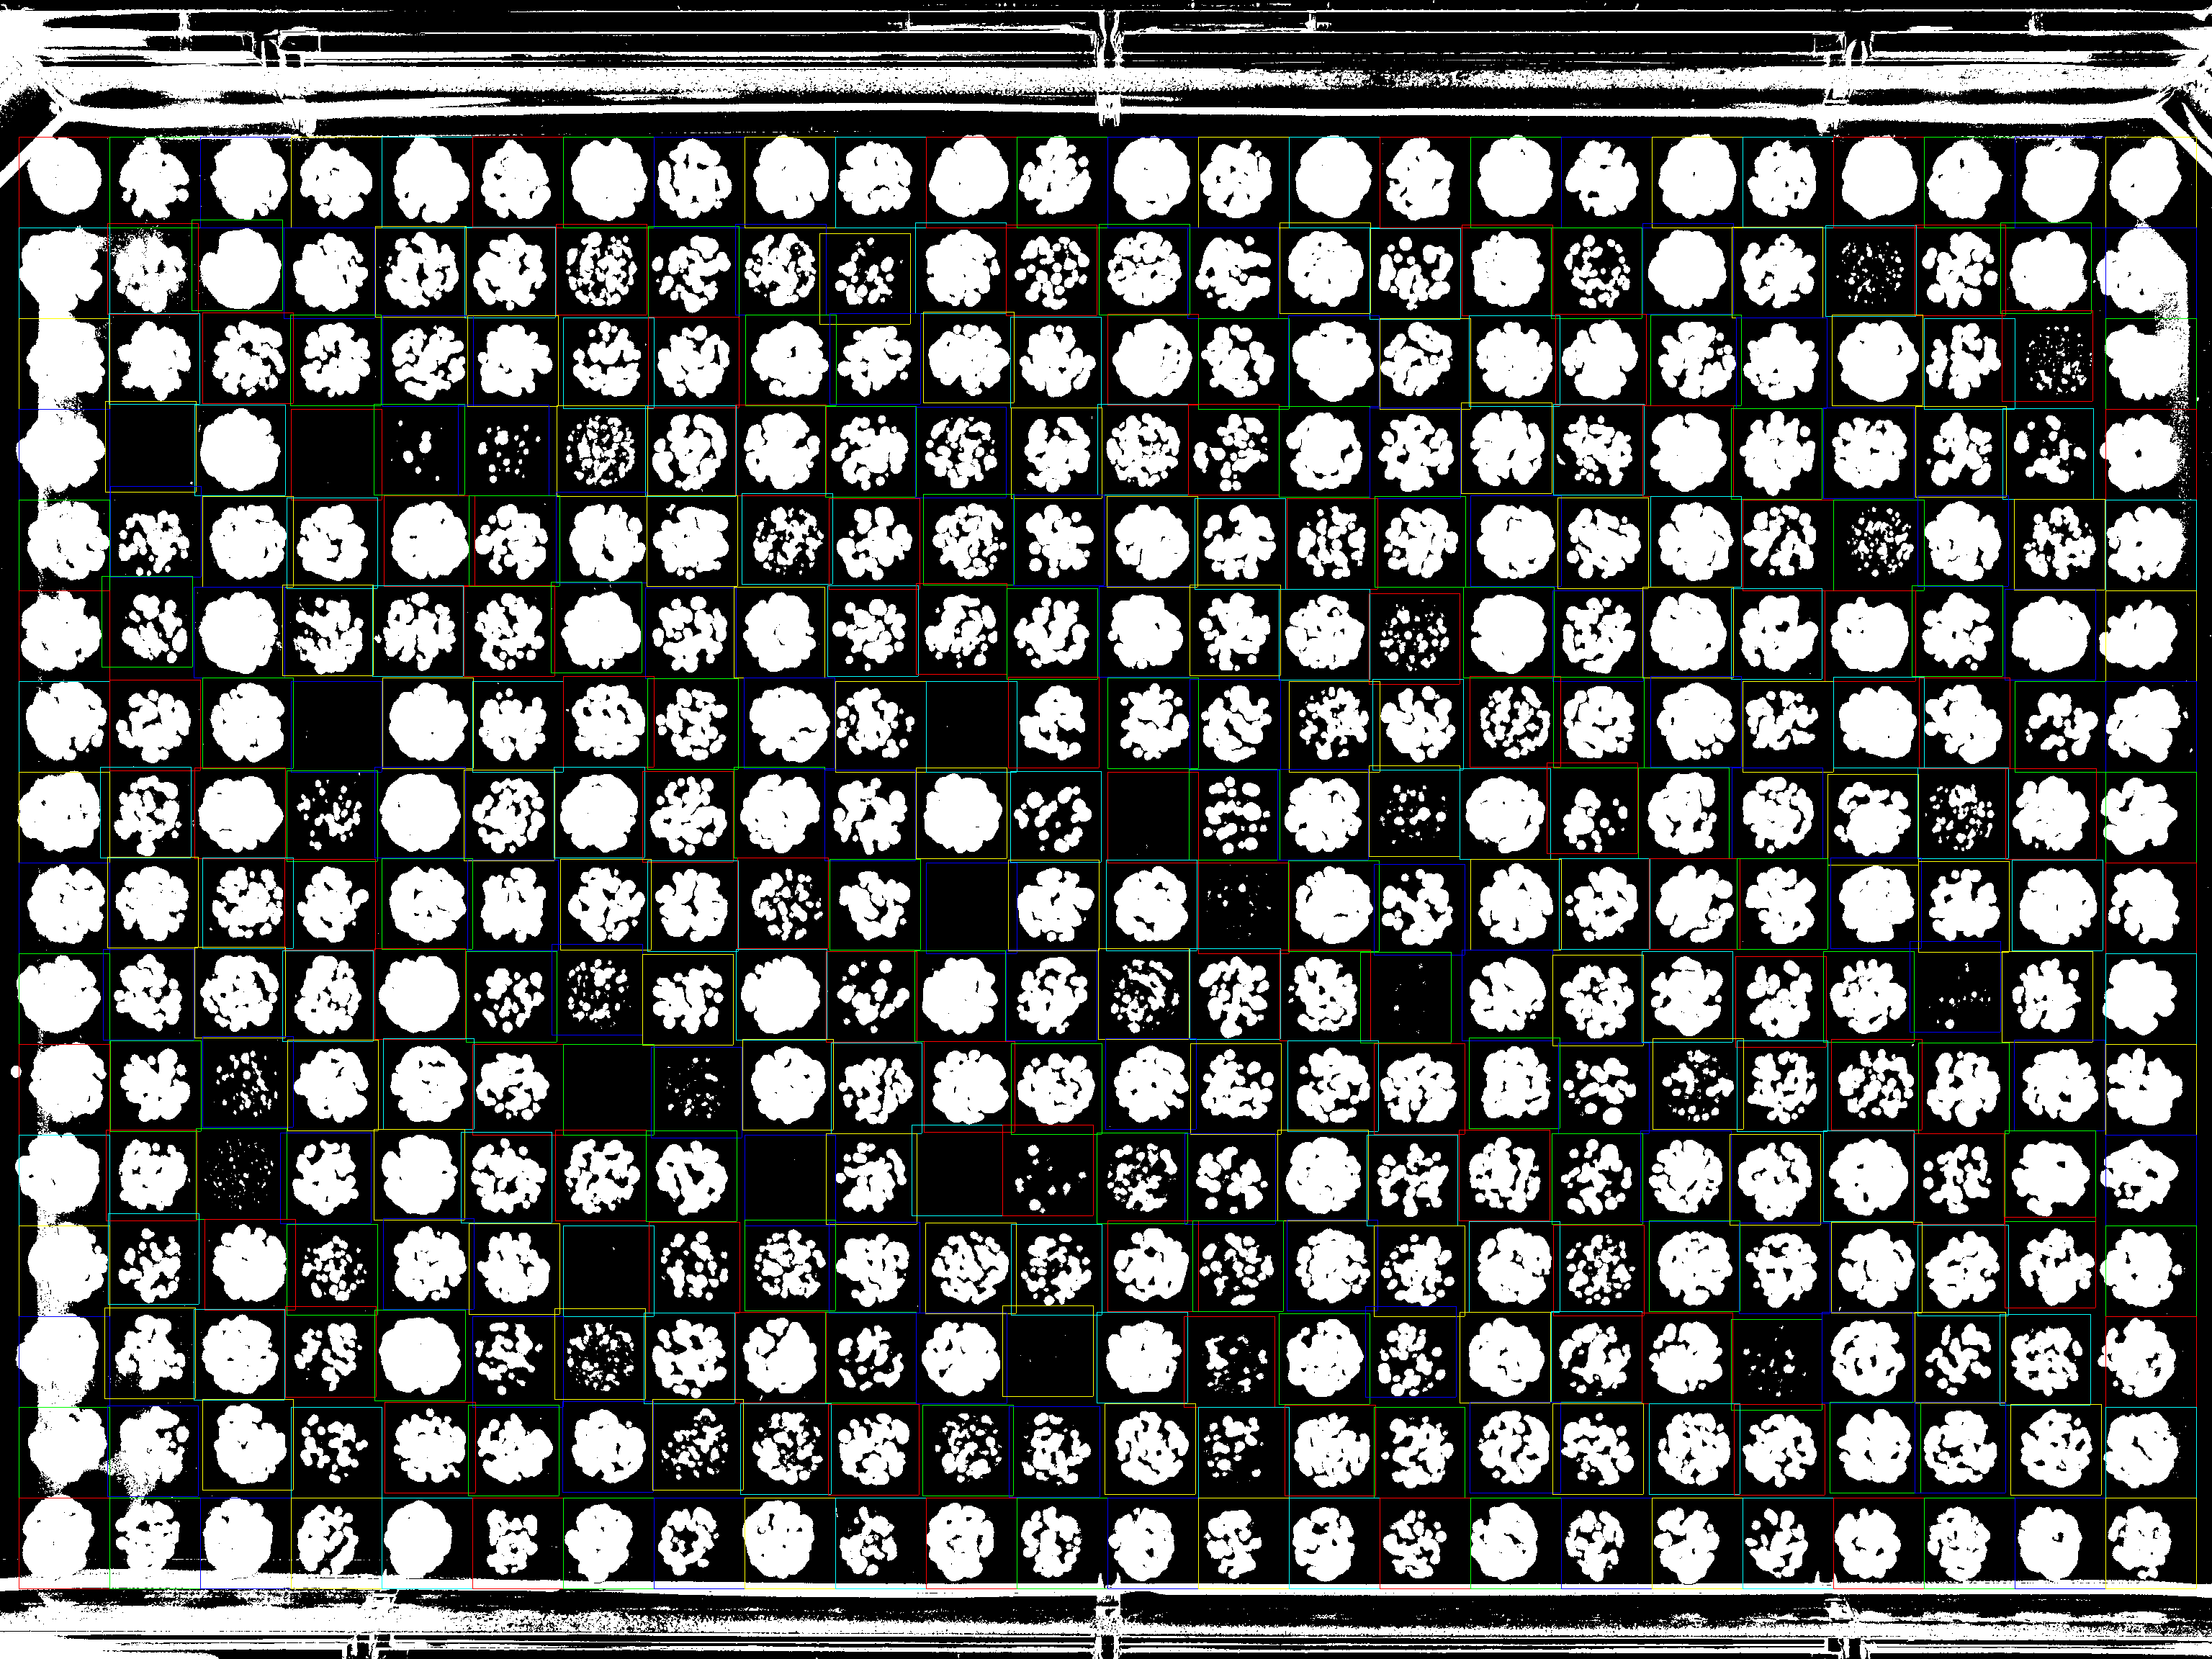
\includegraphics[height=0.4\textheight]{figs/rod-plate-grid-thresh}\hspace{8ex}
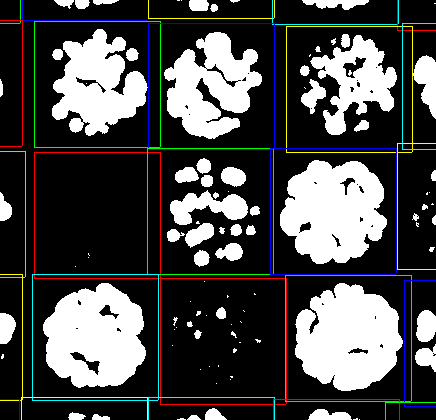
\includegraphics[height=0.4\textheight]{figs/rod-plate-grid-thresh-zoom}

}


\subsection{Growth curve modelling}

\frame{
\frametitle{Growth curve}
\centerline{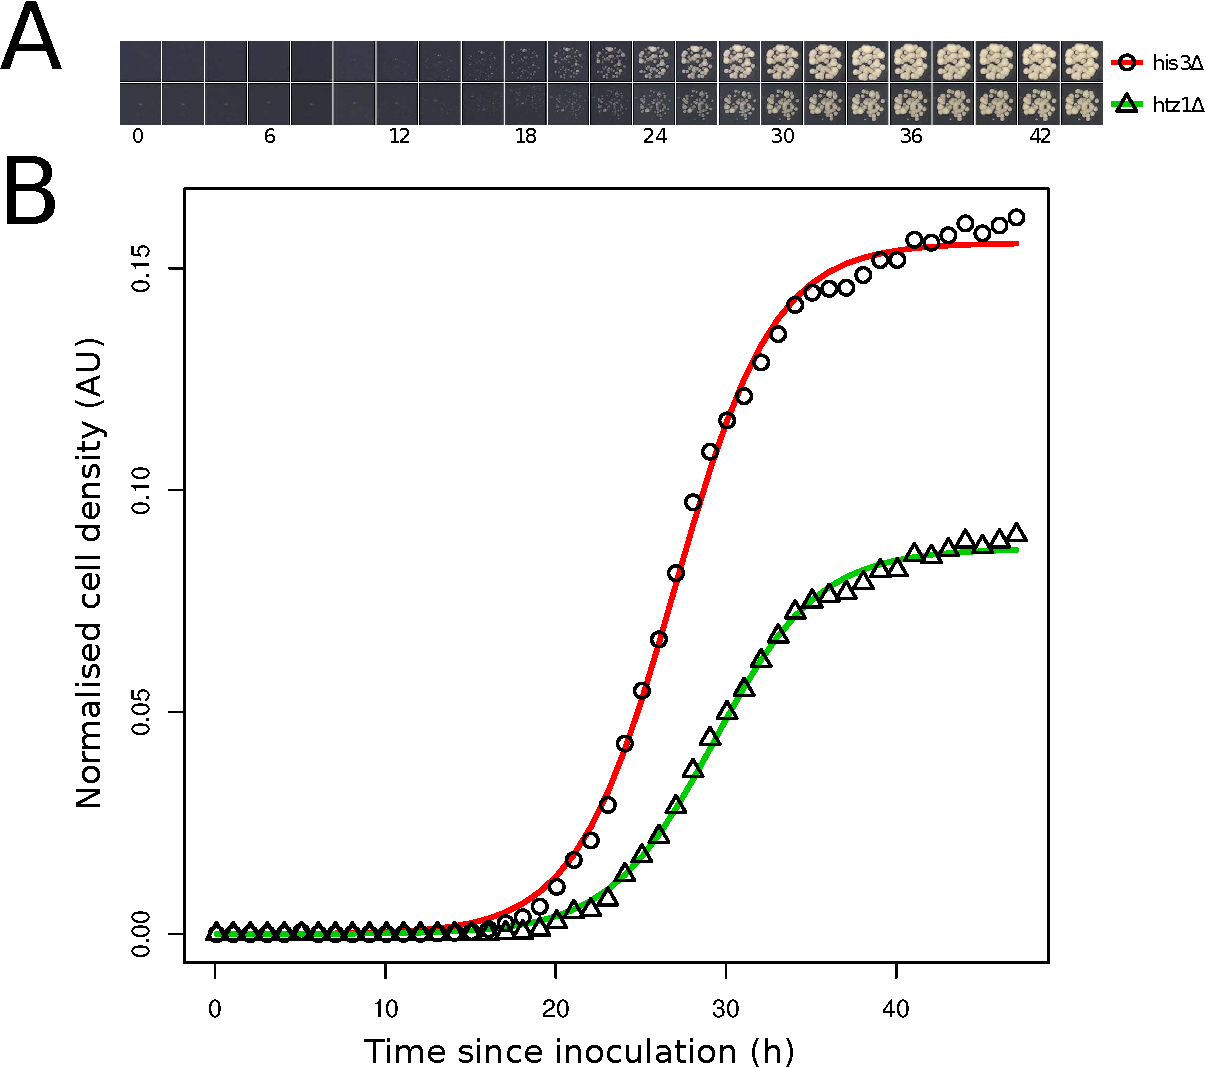
\includegraphics[height=0.8\textheight]{figs/LawlessfigAB}}
%\centerline{\includegraphics[height=0.8\textheight]{figs/ygc1}}
}

\frame{
\frametitle{Growth curve modelling}
\begin{itemize}
\item We want something between a simple smoothing of the data and a
  detailed model of yeast cell growth and division
\item \alert{Logistic growth models} are ideal --- simple
  semi-mechanistic models with interpretable parameters related to
  strain fitness
\item Basic deterministic model:
\[
\frac{dx}{dt} = rx(1-x/K),
\]
subject to initial condition $x=P$ at $t=0$
\item $r$ is the \alert{growth rate} and $K$ is the \alert{carrying capacity}
\item Analytic solution:
\[
x(t) = \frac{KPe^{rt}}{K+P(e^{rt}-1)}
\]
\end{itemize}
}

\frame{
\frametitle{Statistical model}
\begin{itemize}
\item Model observational measurements $\{Y_{t_1},Y_{t_2},\ldots\}$ with
\[
Y_{t_i} = x_{t_i} + \eps_{t_i}
\]
\item Can fit to observed data $y_{t_i}$ using non-linear least
  squares or MCMC
\item Can \alert{fit all (400k) time courses simultaneously} in a large hierarchical
  model which effectively borrows strength, especially across repeats,
  but also across genes
\item Generally works well (fine for most of the downstream scientific
  applications), but fit is often far from perfect...

\end{itemize}
}


\frame{
\frametitle{Fitting the logistic curve}
\centerline{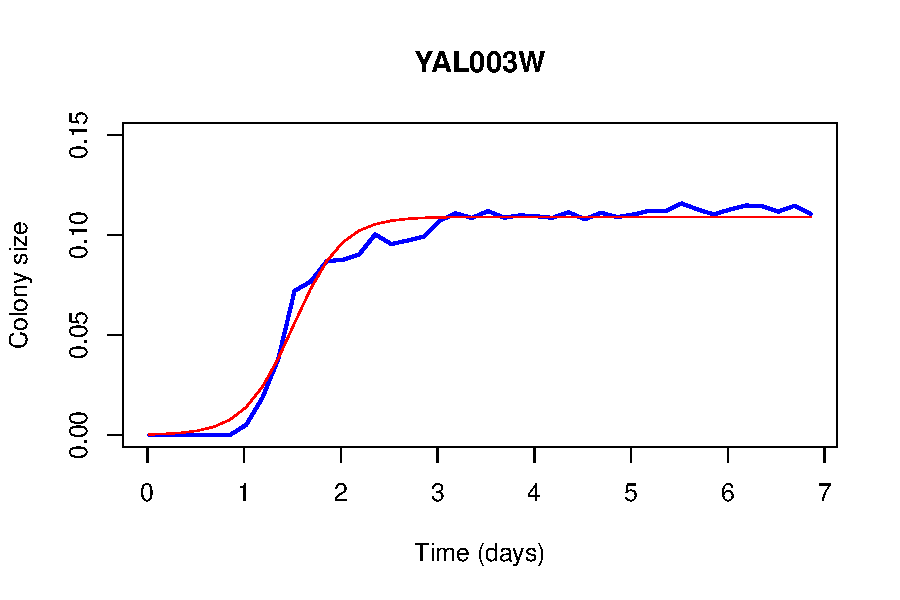
\includegraphics[height=0.8\textheight]{figs/ygc2}}
%Show a bad fit...
}

\frame{
\frametitle{Improved modelling of colony growth curves}
\begin{itemize}
\item Could use a \alert{generalised logistic model} (Richards' 
curve) which
  breaks the symmetry in the shape of ``take off'' and ``landing''
\[
\frac{dx}{dt} = rx(1-(x/K)^\nu)
\]
\item This
  helps, but doesn't address the real problem of strongly
  auto-correlated residuals
\item Better to introduce noise into the dynamics to get a logistic
  growth diffusion process
\end{itemize}
}

\frame{
\frametitle{Stochastic logistic growth diffusion}
\begin{itemize}
\item
Well-known stochastic generalisation of the logistic growth equation,
expressed as an It\^o stochastic differential equation (SDE):
\[
dX_t = rX_t(1-X_t/K)dt + \xi^{-1/2}X_t\,dW_t
\]
\item The \alert{drift} is exactly as for the deterministic model
\item The \alert{diffusion} term injects some noise into the dynamics
\item The \alert{multiplicative noise} ensures that this defines a
  non-negative stochastic process
\end{itemize}
}

\frame{
\frametitle{Sample trajectories from the logistic diffusion}
%\includegraphics[width=0.5\textwidth]{figs/ygc1}
\centerline{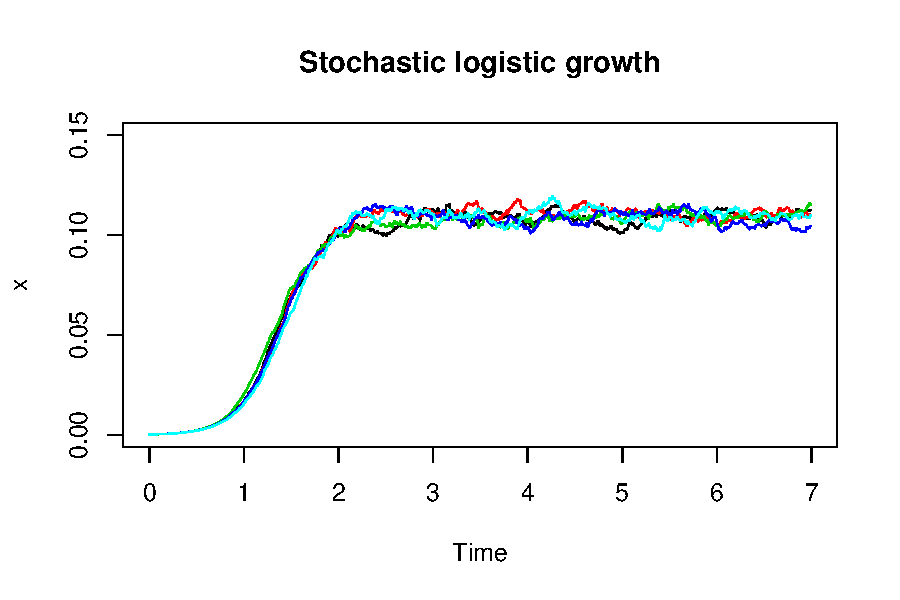
\includegraphics[width=0.8\textwidth]{figs/ygc3}}
}

\frame{
\frametitle{Statistical model}
\begin{itemize}
\item Model observational measurements $\{Y_{t_1},Y_{t_2},\ldots\}$ with
\[
Y_{t_i} = X_{t_i} + \eps_{t_i}
\]
where $X_{t_i}$ refers to our realisation of the diffusion process
\item Need somewhat sophisticated algorithms to fit these sorts of SDE
  models to discrete time data
\item Standard algorithms would require knowledge of the transition
  kernel of the diffusion process, but this is not available for the
  logistic diffusion
\item Lots of work on Bayesian inference for intractable diffusions
  \alert{(Golightly \& W, '05, '06, '08, '10, '11)}, but this won't
  scale to simultaneous fitting of tens of thousands of realisations
\end{itemize}
}

\begin{comment}

\frame{
\frametitle{Approximating the stochastic logistic diffusion}
\begin{itemize}
\item Computational constraints mean that we can only really consider
  working with diffusions having \alert{tractable transition kernels} (as then
  we can apply standard MCMC methods for discrete time problems)
\item If we apply a log transformation to the logistic
  diffusion and then carry out a \alert{linear noise approximation}, the
  result will be a process with log-normal increments
\item Putting $U_t=\log X_t$, It\^o's formula gives
\[
dU_t = \left(r-\frac{1}{2\xi}-\frac{r}{K}e^{U_t}\right)dt + \xi^{-1/2}dW_t
\]
\end{itemize}
}


\frame{
\frametitle{Linear noise approximation (LNA)}
\begin{itemize}
\item Decompose $U_t$ into a deterministic component and a stochastic
  residual process
\[
U_t = v_t + Z_t
\]
where $v_t$ solves the deterministic part
\[
\frac{dv_t}{dt} = r-\frac{1}{2\xi}-\frac{r}{K}e^{v_t}
\]
\item Subtracting out the deterministic solution from $U_t$ leaves a
  residual process of the form
\[
dZ_t = \frac{r}{K}e^{v_t}(1-e^{Z_t})dt+\xi^{-1/2}dW_t
\]
\end{itemize}
}

\frame{
\frametitle{Linear noise approximation (LNA)}
\begin{itemize}
\item Applying the \alert{linear approximation} $1-e^{Z_t}\simeq -Z_t$
  to linearise the drift gives
\[
dZ_t = -\frac{r}{K}e^{v_t}Z_tdt+\xi^{-1/2}dW_t
\]
\item Substituting in for $v_t$ then gives
\[
dZ_t = -\frac{abPe^{at}}{bP(e^{at}-1)+a}Z_tdt+\xi^{-1/2}dW_t,
\]
where $a=r-1/(2\xi)$ and $b=r/K$
\item This is a (zero) mean-reverting time-varying
  \alert{Ornstein--Uhlenbeck} (OU) process, and can
  be solved exactly, giving a normal transition kernel
\end{itemize}
}

\frame{
\frametitle{The logistic diffusion and the LNA}
\includegraphics[width=0.5\textwidth]{figs/ygc4}
\includegraphics[width=0.5\textwidth]{figs/ygc6}

The (log)LNA is a very good approximation to the true process, with
\alert{tractable log-normal increments}
}

\end{comment}

\frame{
\frametitle{Further simplifications and approximations}
\begin{itemize}
\item The \alert{linear noise approximation} (LNA) applied to the log-transformed process is a good model with a tractable transition kernel
\item We can implement standard discrete time MCMC methods to estimate
  model parameters together with the unobserved latent trajectories
\item Embedding in a hierarchical model is straightforward
\item These methods work fine for hundreds of growth curves, but are
  still problematic for tens of thousands of growth curves
\end{itemize}
}

\frame{
\frametitle{Integrating out the latent process}
\begin{itemize}
  \item If we are prepared to assume linear Gaussian error on the log
    scale, we can use \alert{Kalman filtering} techniques to \alert{integrate out} the
    latent process (but this isn't very plausible)
  \item Alternatively, we could apply a LNA directly to the logistic
    diffusion (without first transforming), and assume linear Gaussian
    error on that scale (\alert{Heydari et al, 2013})
  \item This latter approach turns out to be better, despite the fact that the LNA approximation to the true process isn't quite as good
\item More important to have a plausible error structure than a super-accurate approximation to the stochastic process
\end{itemize}
}

\frame{
\frametitle{Growth curve model}
\centerline{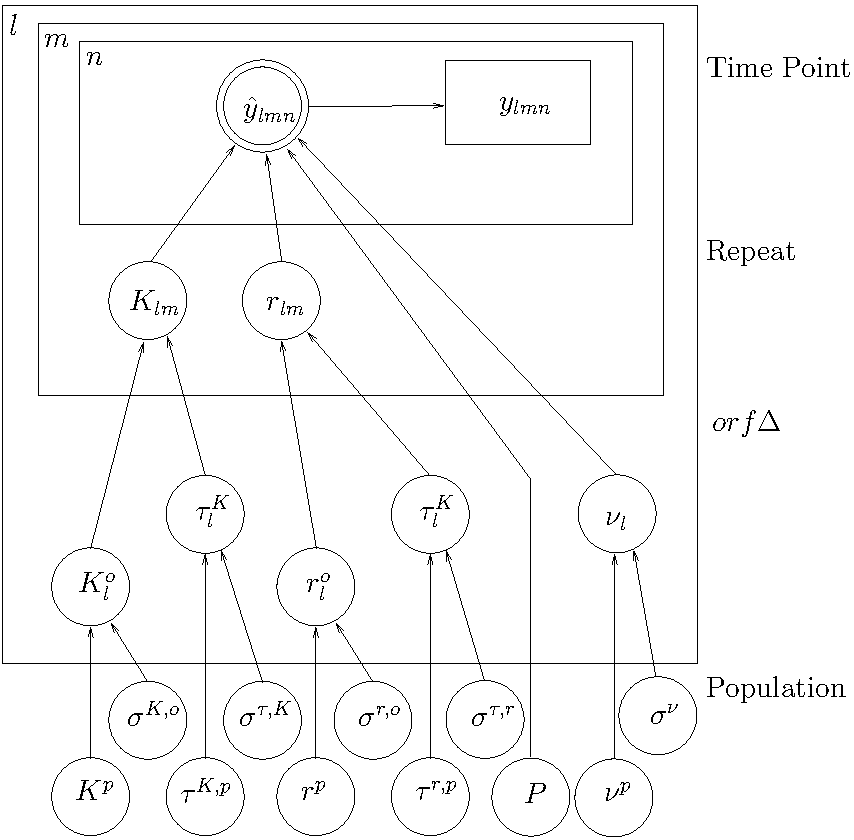
\includegraphics[height=0.8\textheight]{figs/DAG1}}
}

\frame{
\frametitle{Colony fitness}
\begin{itemize}
\item The results of model fitting are estimates (or posterior
  distributions) of $r$ and $K$ for each yeast colony, and also the
  corresponding gene level parameters
\item Both $r$ and $K$ are indicative of colony fitness --- keep
  separate where possible
\item Often useful to have a scalar measure of fitness --- many
  possibilities, including $rK$, $r\log K$, or MDR$\times$MDP, where
  MDR is the
  maximal doubling rate and MDP is the maximal doubling potential
\item Statistical summaries can be fed in as data to the next
  level of analysis (or, ultimately, modelled jointly as a giant
  hierarchical model)
\end{itemize}
}

\subsection{Modelling genetic interaction}

\frame{
\frametitle{Epistasis}
From Wikipedia:
\begin{itemize}
\item \emph{``\alert{Epistasis is the interaction between
genes}. Epistasis takes place when the action of one gene is modified
by one or several other genes, which are sometimes called modifier
genes. The gene whose phenotype is expressed is said to be epistatic,
while the phenotype altered or suppressed is said to be hypostatic.''}
\item \emph{``\alert{Epistasis and genetic interaction refer to the same
phenomenon}; however, epistasis is widely used in population genetics
and refers especially to the statistical properties of the
phenomenon.''}
\end{itemize}
}

\frame{
\frametitle{Multiplicative model}
\begin{itemize}
\item Consider two genes with alleles $a/A$ and $b/B$ with $a$ and
$b$ representing ``wild type'' (note that $A$ and $B$ could potentially
represent knock-outs of $a$ and $b$) 
\item Four genotypes: aa, Ab, aB, AB. Use $[\cdot]$ to denote some
  quantitative phenotypic measure (eg. ``fitness'') for each genotype
\item \alert{Multiplicative model} of genetic independence:
\begin{tabbing}
$[AB]\times [ab] = [Ab]\times [aB]$ \qquad\= no epistasis \\
$[AB]\times [ab] > [Ab]\times [aB]$ \qquad\= synergistic epistasis \\
$[AB]\times [ab] < [Ab]\times [aB]$ \qquad\= antagonistic epistasis 
\end{tabbing}
\item Perhaps simpler if re-written in terms of relative fitness:
\[
\frac{[AB]}{[ab]} = \frac{[Ab]}{[ab]}\times \frac{[aB]}{[ab]}
\]
\end{itemize}
}

\frame{
\frametitle{Genetic independence and HTP data}
\begin{itemize}
\item Suppose that we have scaled our data so that it is
consistent with a multiplicative model --- what do we expect to see?
\item The independence model $[AB]\times [ab] = [Ab]\times [aB]$ translates to
\[
[\text{query}:\text{abc}\Delta] \times [\text{wt}] = [\text{query}] \times
[\text{abc}\Delta]\]
\item In other words
\[
[\text{query}:\text{abc}\Delta]  = \frac{[\text{query}]}{[\text{wt}]} \times
[\text{abc}\Delta]\]
\item That is, the double-mutant differs from the single-deletion by a
constant multiplicative factor that is independent of the particular
single-deletion
\item ie. a scatter-plot of double against single will show them all
lying along a straight line
\end{itemize}
}

\frame{
\frametitle{Statistical modelling}
\begin{itemize}
\item
Assume that $F_{clm}$ is the fitness measurement for repeat $m$ of
gene deletion $l$ in condition $c$ ($c=1$ for the single deletion and
$c=2$ for the corresponding double-mutant)
\item Model:
\begin{align*}
F_{clm} &\sim N(\hat{F}_{cl},1/\nu_{cl}) \\
\log \hat{F}_{cl} &= \alpha_c + Z_l + \delta_l\gamma_{cl} \\
\delta_l &\sim Bern(p)
\end{align*}
\item $\delta_l$ is a variable selection indicator of \alert{genetic
    interaction}
\item Then usual Bayesian hierarchical stuff...
\end{itemize}
}

\frame{
\frametitle{Genetic interaction model}
\centerline{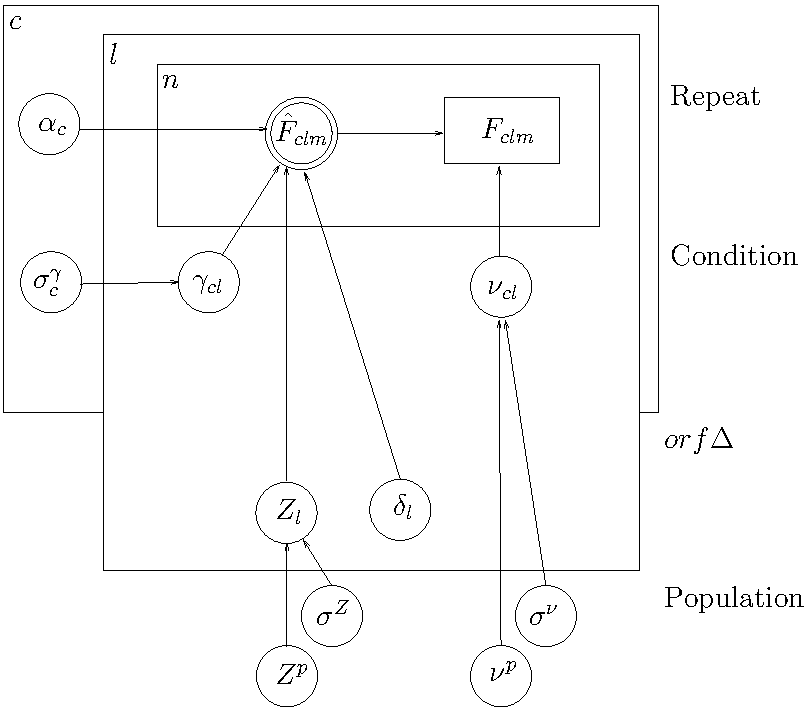
\includegraphics[height=0.8\textheight]{figs/DAG2}}
}

\frame{
\frametitle{Genetic interaction results}
\centerline{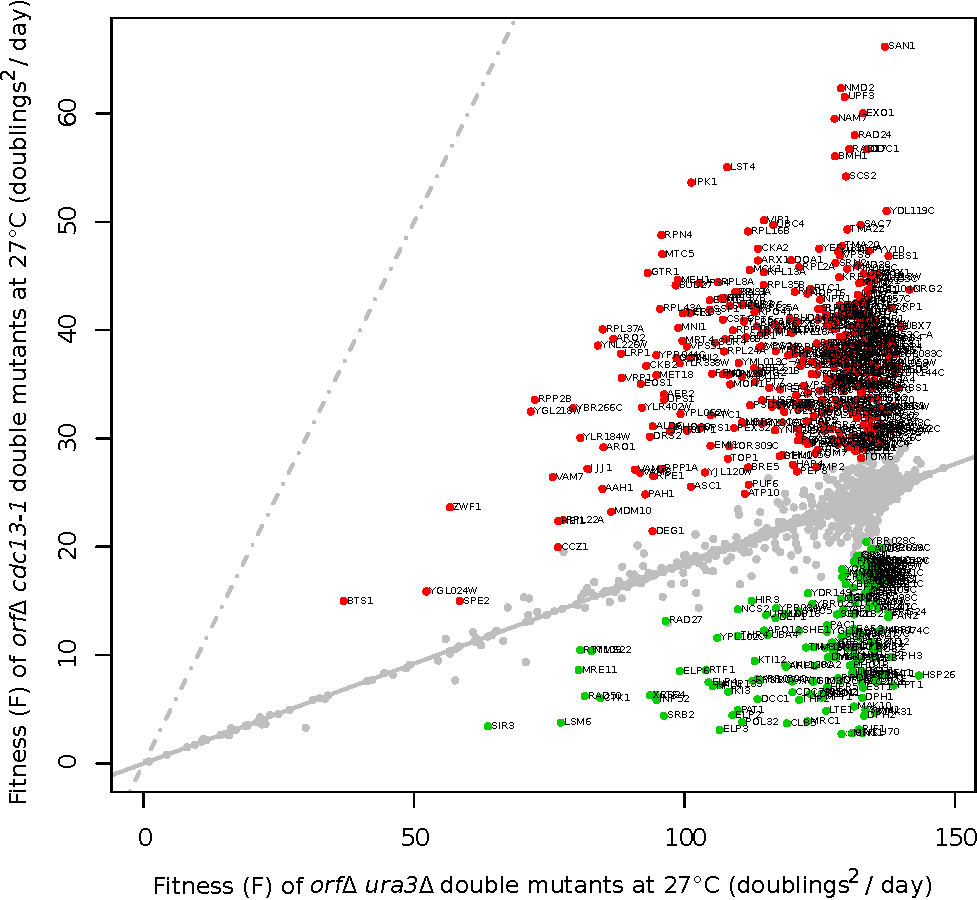
\includegraphics[height=0.8\textheight]{figs/IHM}}
}

\frame{
\frametitle{Joint modelling of growth curves and genetic interaction}
\begin{itemize}
\item We can integrate together the hierarchical growth curve model
  and the genetic interaction model into a combined joint model
\item This has usual advantages of properly borrowing strength, proper
  propagation of uncertainty, etc.
\item Also very convenient to avoid requiring a scalar measure of
  ``fitness''
\item If $y_{clmn}$ is the colony size at time point $n$ in repeat $m$
  of gene $l$ in condition $c$, then
\begin{align*}
y_{clmn} &\sim N(\hat{y}_{clmn},1/\nu_{cl}) \\
\hat{y}_{clmn} &= X(t_{clmn};K_{clm},r_{clm},P) \\
\log K_{clm} &\sim
N(\alpha_c+K_l^o+\delta_l\gamma_{cl},1/\tau_{cl}^K)\\
\log r_{clm} &\sim N(\beta_{c}+r_l^o+\delta_l\omega_{cl},1/\tau_{cl}^r)
\end{align*}
\end{itemize}
}

\frame{
\frametitle{Joint model}
\centerline{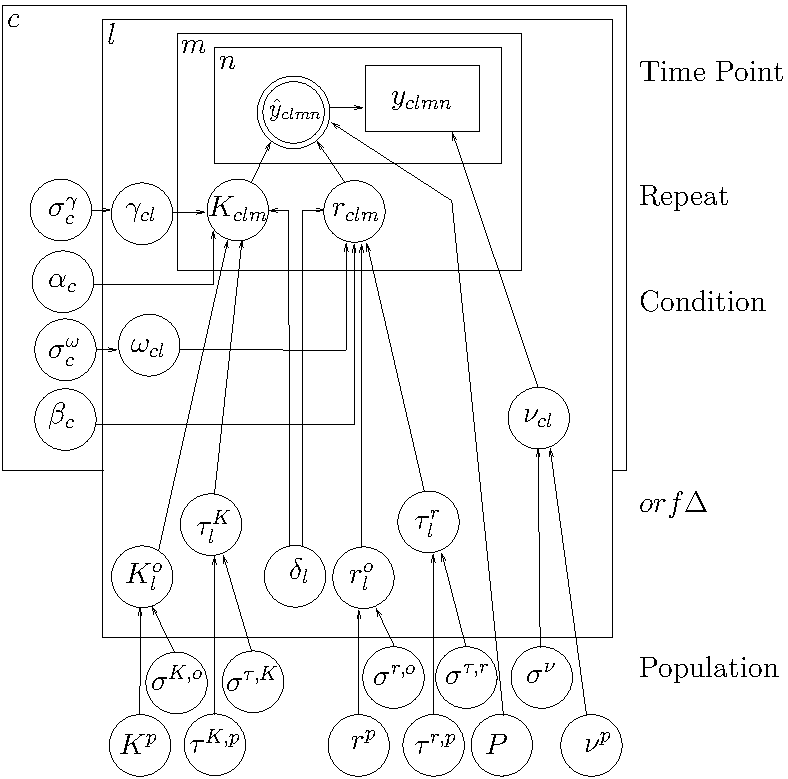
\includegraphics[height=0.8\textheight]{figs/DAG3}}
}

\frame{
\frametitle{Joint model results}
\centerline{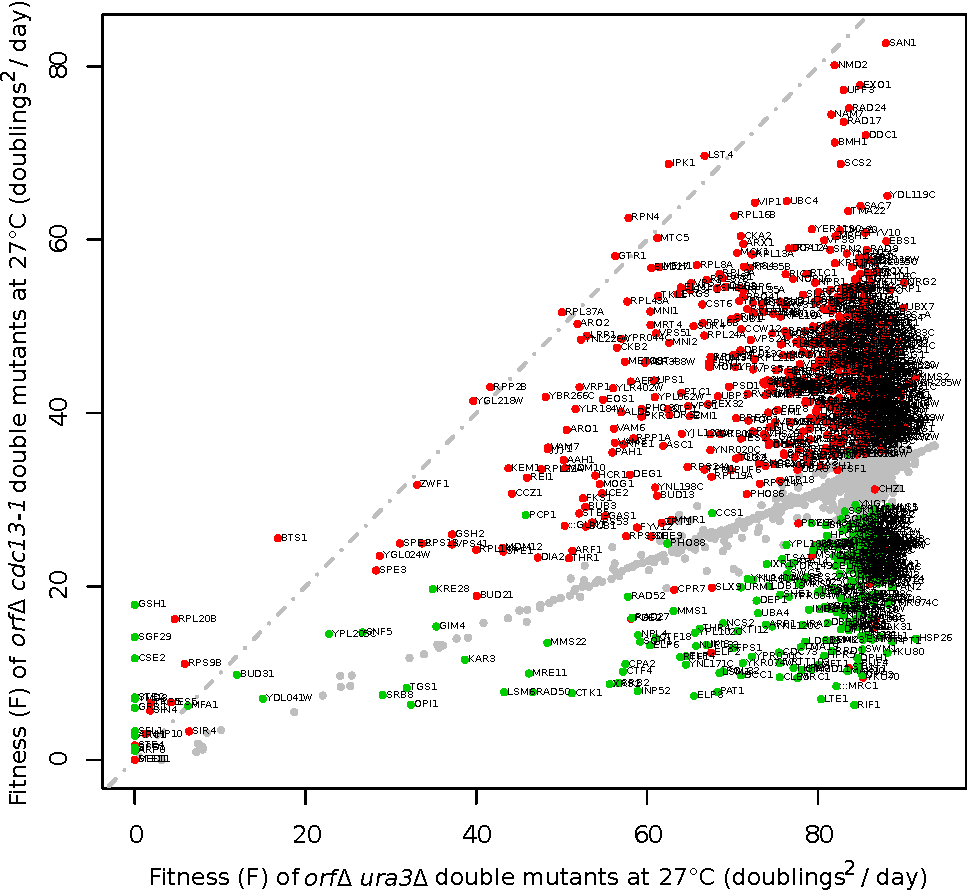
\includegraphics[height=0.8\textheight]{figs/JHM}}
}

\subsection{MiniQFA}

\frame{
\frametitle{MiniQFA}
Not just a single query, but an ``all-by-all" experiment for a (small) subset of the genome
  \begin{itemize}
  \item We have run an experiment with 150 gene knockouts (in both wt and cdc13-1 backgrounds) on a single plate, using each in turn as the query mutation, to map out the full set of pairwise interactions for the subset
  \item Requires an extension and some modification of the previous hierarchical models
  \item Enables an in depth study of the prevelance of genetic interaction, and will allow consideration of alternative notions of genetic interaction and epistasis, which could distinguish between ``direct" and ``indirect" interactions
  \end{itemize}
%\end{itemize}
}

\frame{
\frametitle{MiniQFA model}
\begin{itemize}
\item Initial modelling approach based on two stages
\item Interaction model:
\begin{align*}
F_{ll'm} &\sim N(\hat{F}_{ll'm},1/\nu)\\
\log \hat{F}_{ll'm} &= \mu + Z_l + Z_{l'} + \delta_{ll'}\gamma_{ll'} \\
\delta_{ll'} &\sim \text{Bern}(p)
\end{align*}
\item A version assuming symmetry (eg. $\delta_{ll'}=\delta_{l'l}$, and similar for $\gamma_{ll'}$), and another which doesn't, another with $t$ errors, ...
\item Using preliminary data, only around 10\% of the $\binom{150}{2}\simeq 11$k potential interactions are being selected
\item Starting to think about implementation of the ``direct" versus ``indirect" model...
\end{itemize}
}

\frame{
\frametitle{Preliminary MiniQFA results (cdc13-1 at 27C)}
\centerline{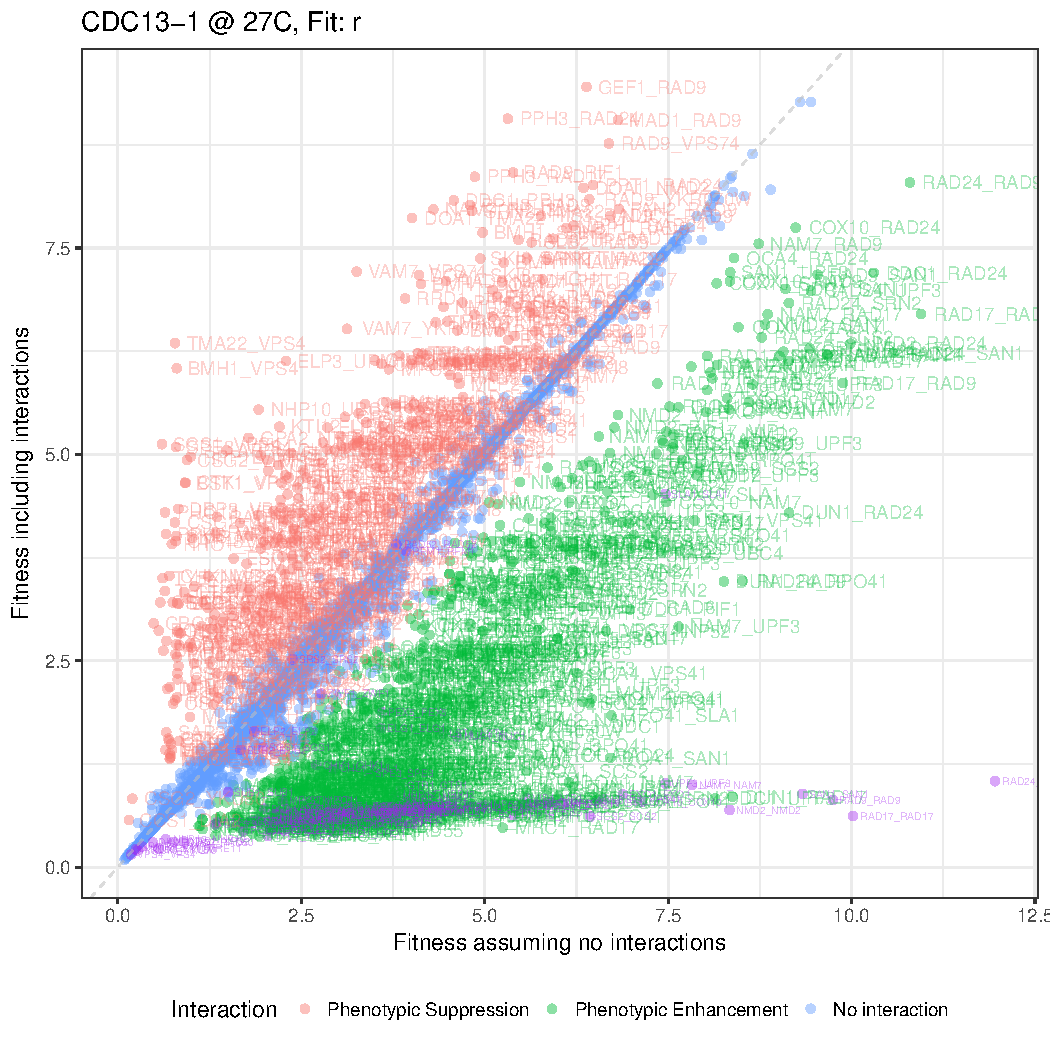
\includegraphics[height=0.9\textheight]{figs/mQFA_GISplot_FitCDC13D127}}
}

\frame{
\frametitle{All double deletions}
\centerline{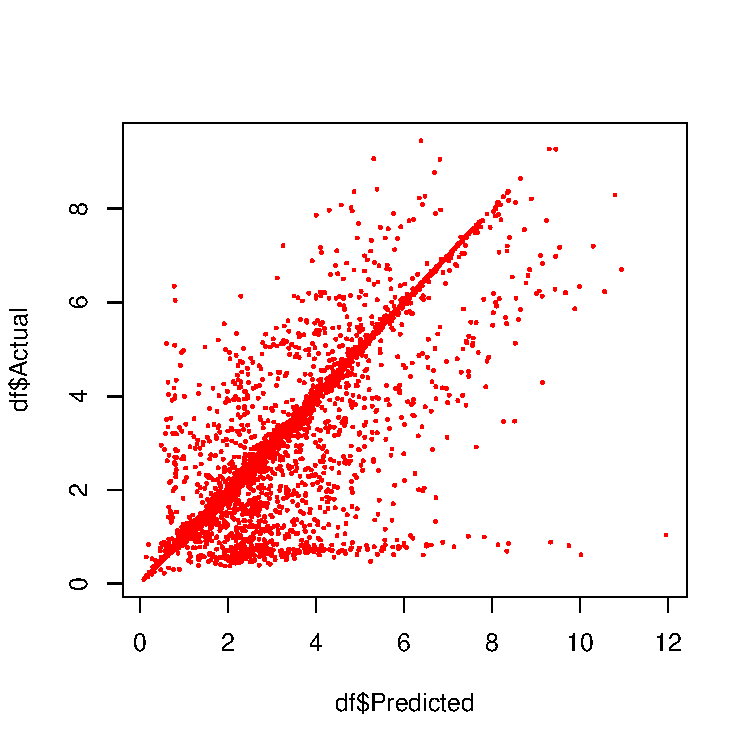
\includegraphics[height=0.9\textheight]{figs/mqfa-all}}
}

\frame{
\frametitle{Only the interacting double deletions}
\centerline{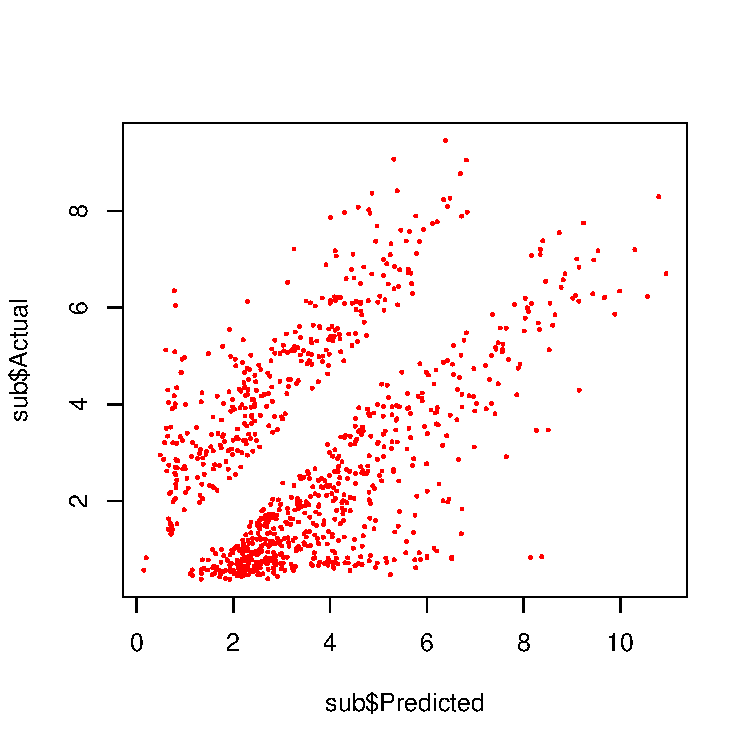
\includegraphics[height=0.9\textheight]{figs/mqfa-int}}
}

\frame{
\frametitle{Graph of pairwise interactions}
\centerline{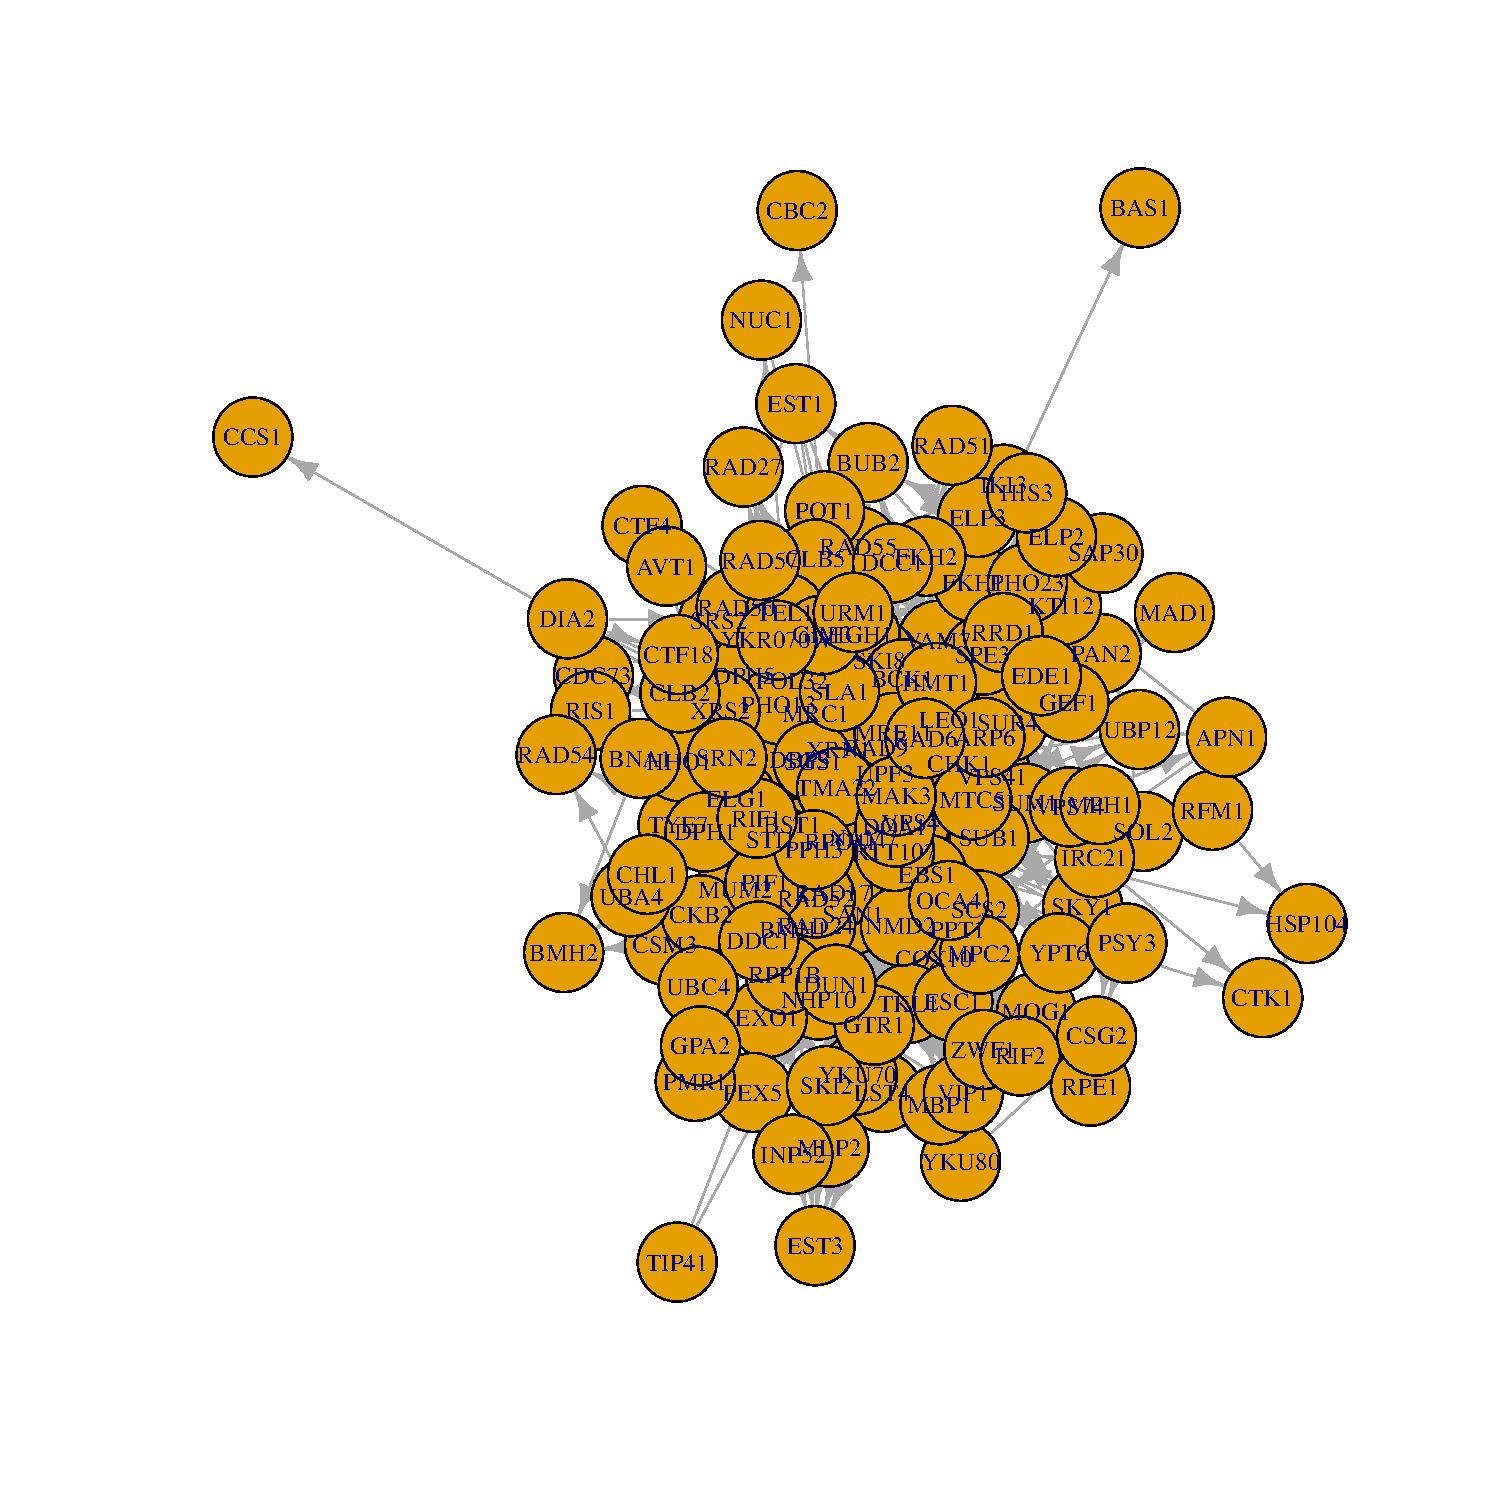
\includegraphics[height=0.9\textheight]{figs/mqfa-dag}}
}

\frame{
\frametitle{Circle layout}
\centerline{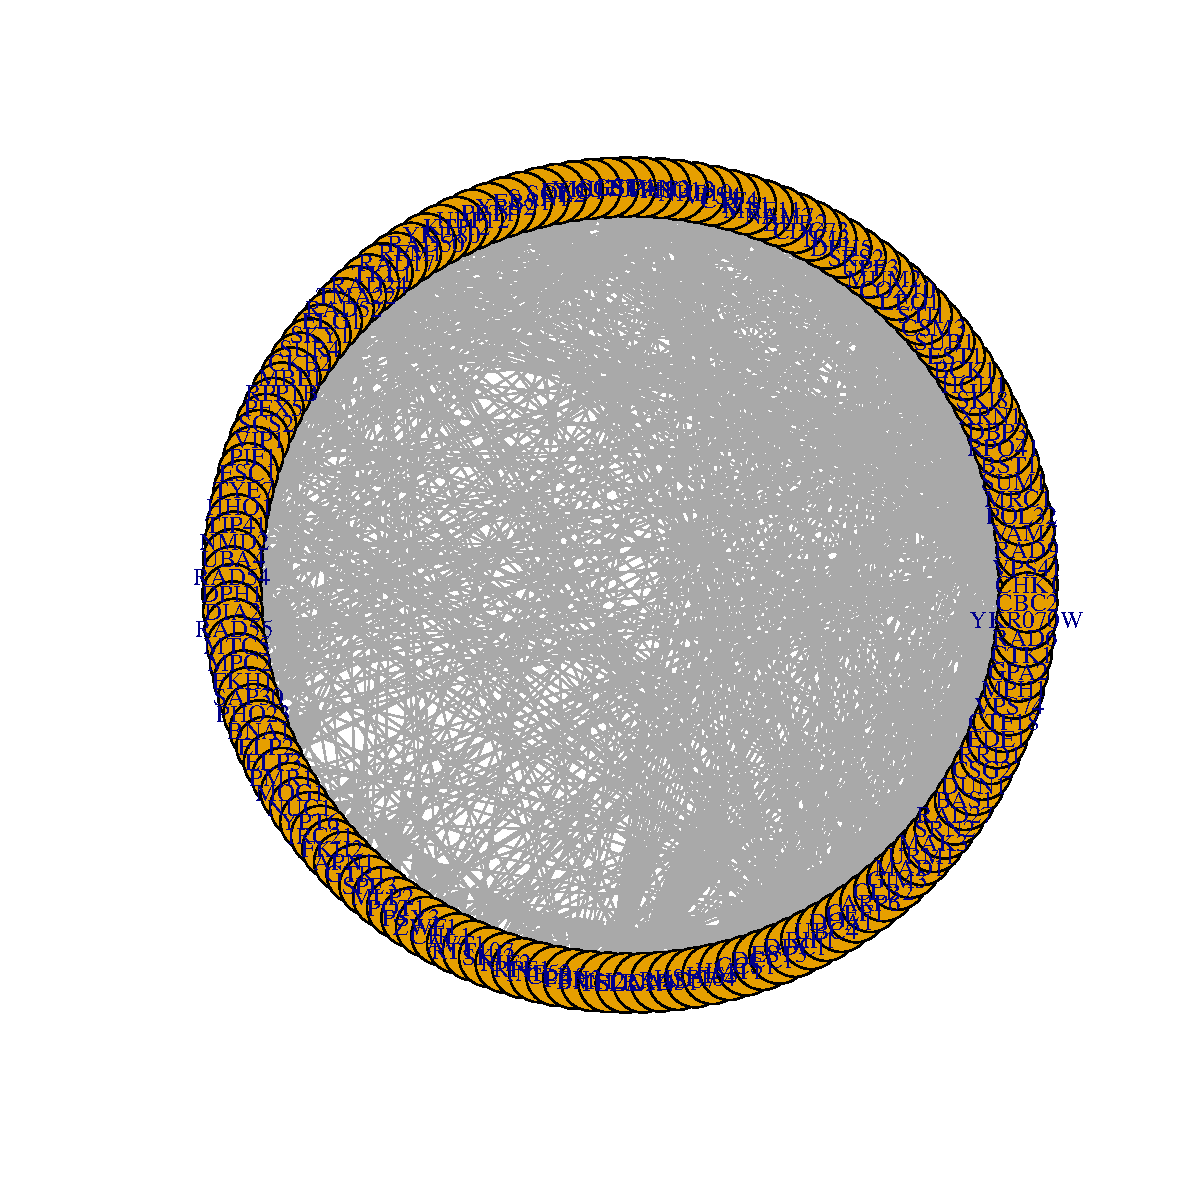
\includegraphics[height=0.9\textheight]{figs/mqfa-circ}}
}

\frame{
\frametitle{Adjacency matrix}
\centerline{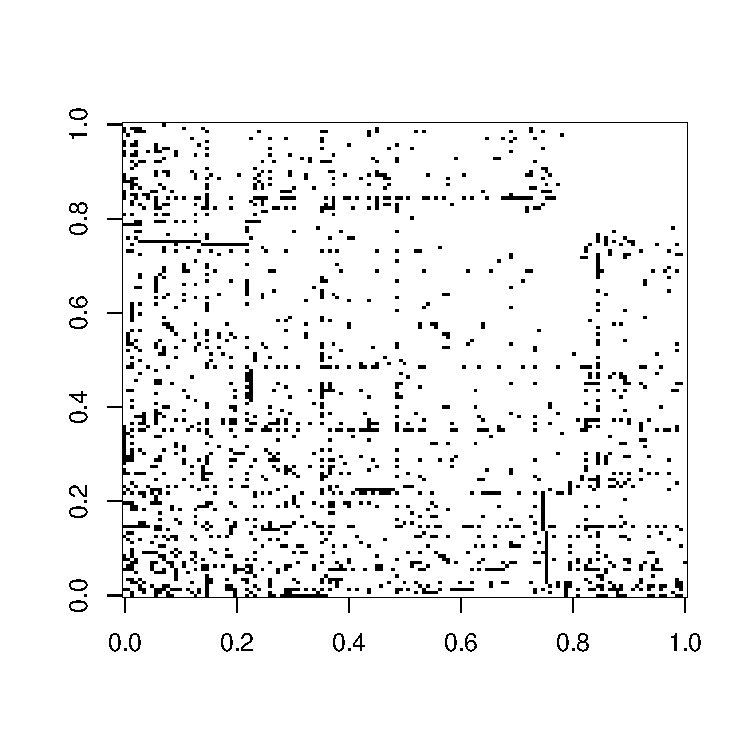
\includegraphics[height=0.9\textheight]{figs/mqfa-adj}}
}

\frame{
\frametitle{Adjacency matrix (``fast greedy'' graph clustering)}
\centerline{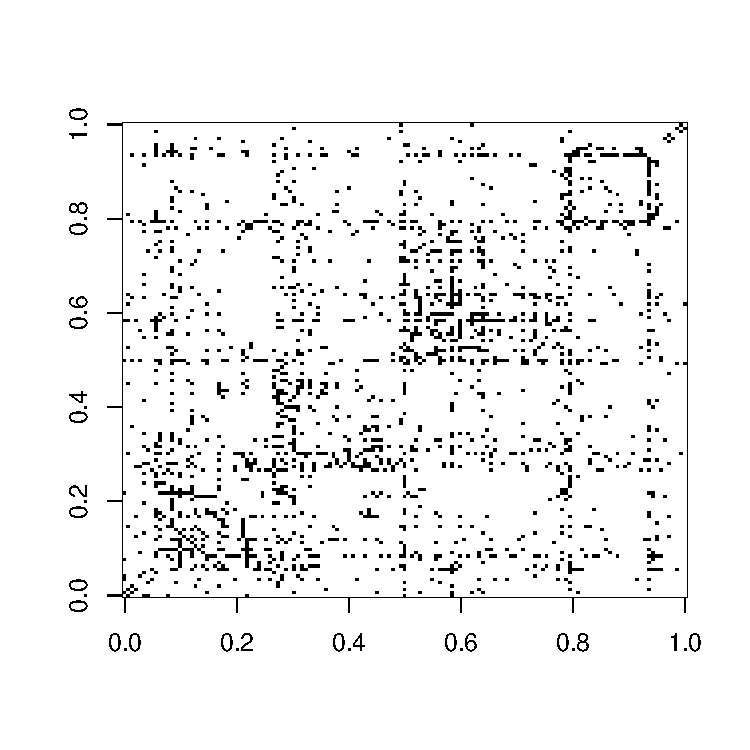
\includegraphics[height=0.9\textheight]{figs/mqfa-adj-fg}}
}

\frame{
\frametitle{Interaction graph (``fast greedy'' graph clustering)}
\centerline{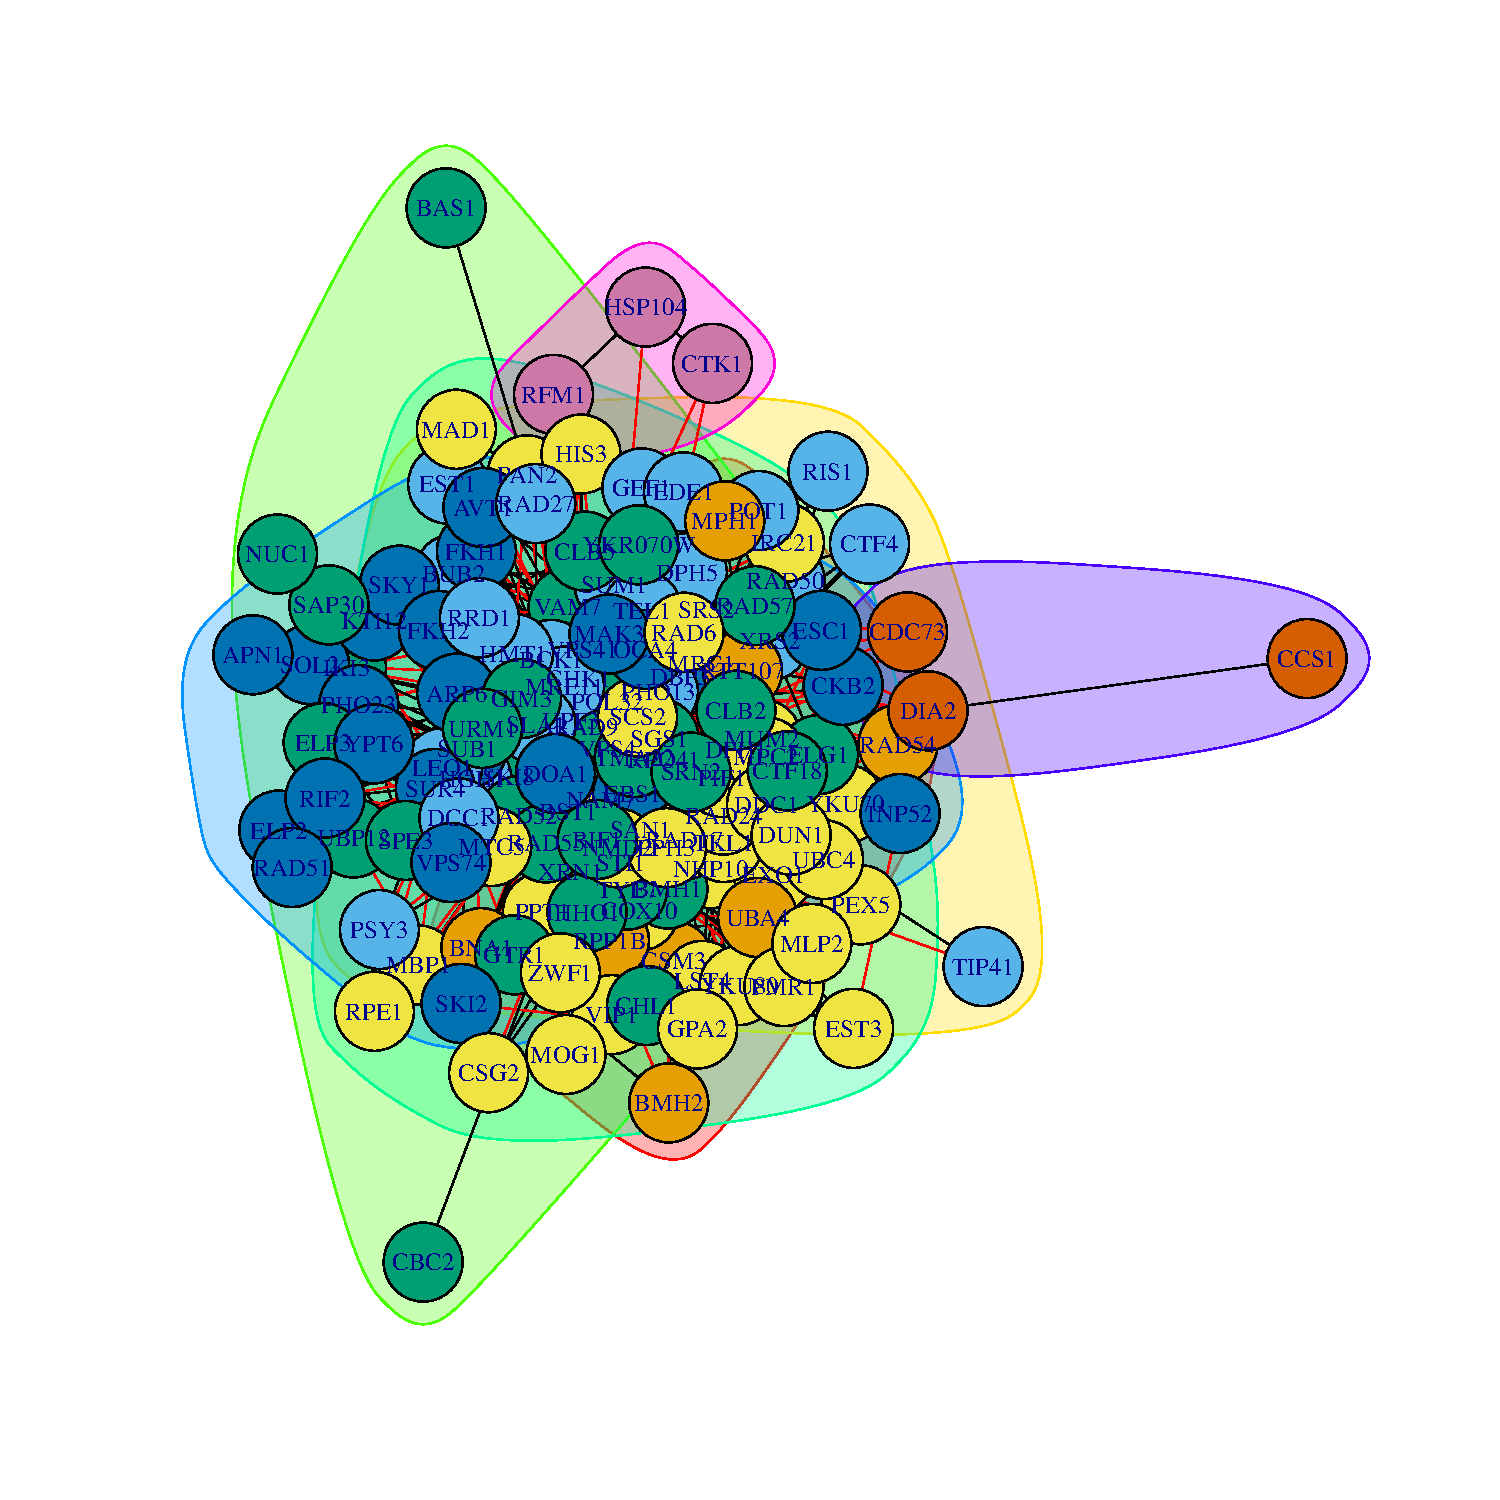
\includegraphics[height=0.9\textheight]{figs/mqfa-ug-fg}}
}

\frame{
\frametitle{Adjacency matrix (``spin--glass'' graph clustering)}
\centerline{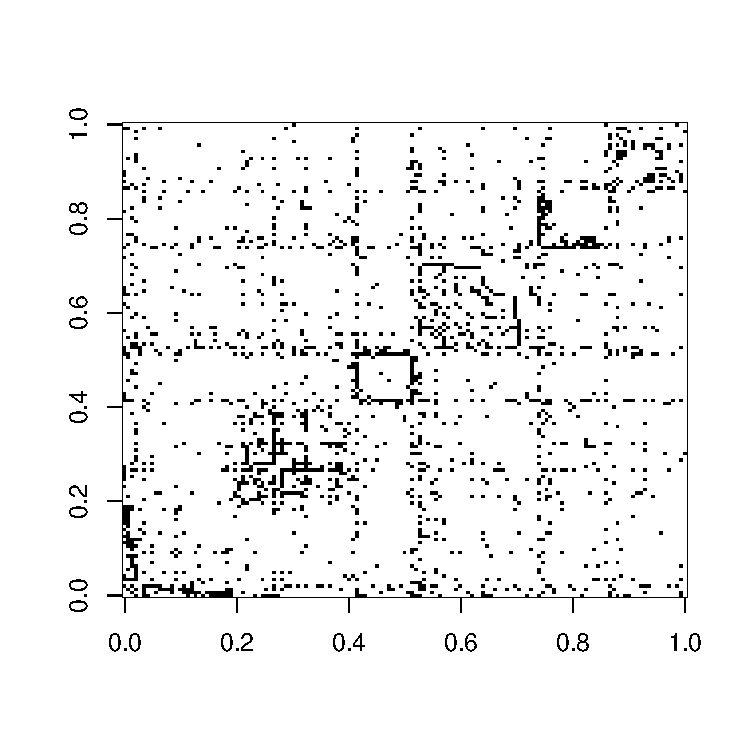
\includegraphics[height=0.9\textheight]{figs/mqfa-adj-sg}}
}

\frame{
\frametitle{Interaction graph (``spin--glass'' graph clustering)}
\centerline{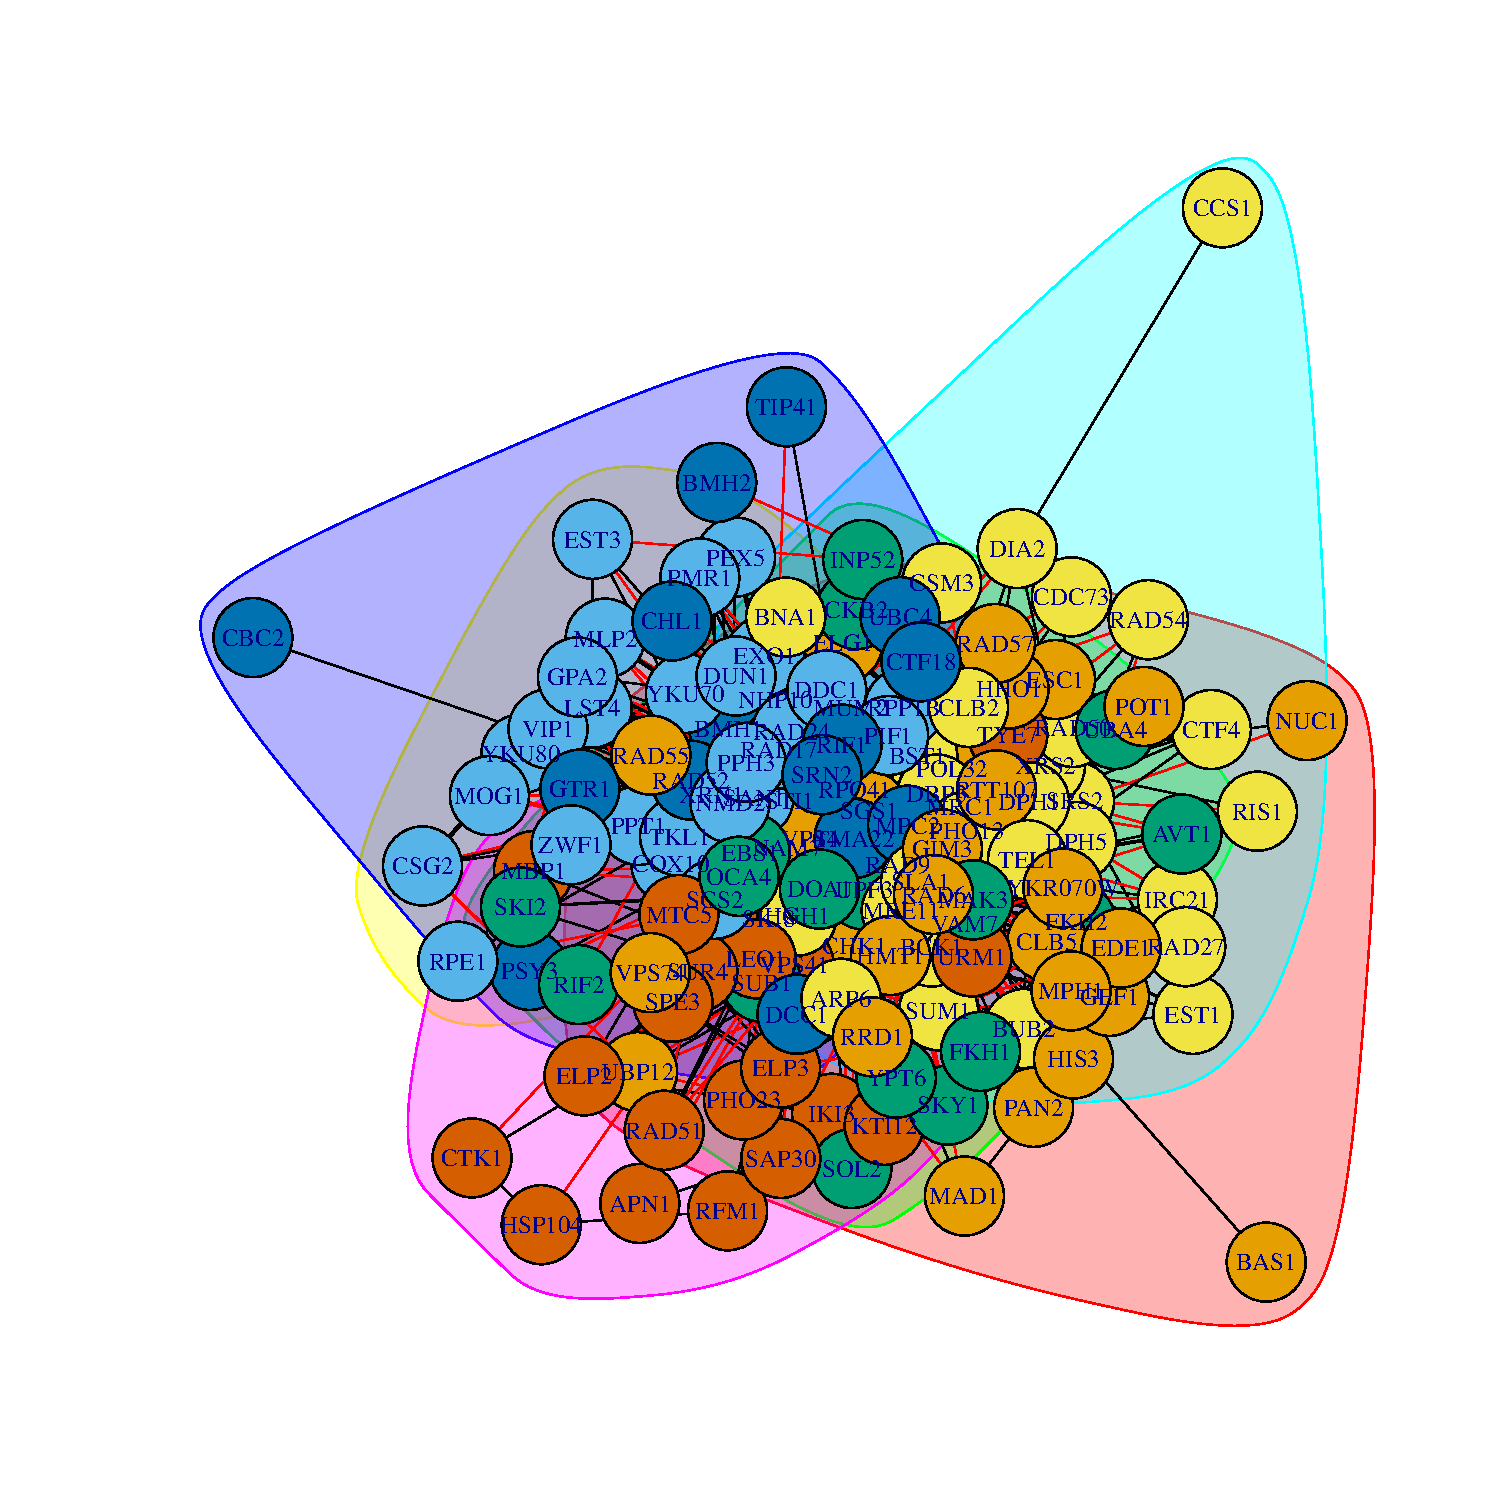
\includegraphics[height=0.9\textheight]{figs/mqfa-ug-sg}}
}

\section{Summary and conclusions}
%\section{Computational issues}

\begin{comment}
  
% \subsection{``Big data'' issues}

\frame{
\frametitle{``Big data'' issues}
\begin{itemize}
\item Understanding \alert{conflict} between model and data in big data contexts --- does more data demand \alert{more complex models}?
\item Model \alert{simplifications} and improvements to MCMC (linear Gaussian block updates and proposals, ``INLA proposals'', 2-block proposals, reparameterisations, GVS, etc.)
\item Basic \alert{parallelisation} strategies (parallel chains, parallellelised single chain)
\item Investigation of \alert{data parallel} strategies (consensus Monte Carlo, etc.)
\item Novel representations, interpretations and implementations of Bayesian hierarchical models using ideas from \alert{probabilistic programming} and strongly typed \alert{functional programming languages} (Scala, Haskell, Eta, OCaml, ...)
\end{itemize}
}

\end{comment}

\subsection{Summary}

\frame{
\frametitle{Summary}
\begin{itemize}
\item Modern bioscience is generating large, complex data sets which
  require \alert{sophisticated modelling} in order to answer questions of
  scientific interest
\item Big data forces \alert{trade-offs} between statistical accuracy and
  computational tractability
\item \alert{Stochastic dynamic models} are much more flexible than deterministic
  models, but come at a computational cost --- the LNA can
  sometimes represent an excellent compromise
\item Notions of \alert{genetic interaction} translate directly to statistical
  models of interaction
\item Big hierarchical \alert{variable selection} models are useful in genomics, but can be computationally challenging
\end{itemize}
}


\begin{comment}
  
\frame{
\frametitle{Funding acknowledgements}
Major funders of this work:
\begin{itemize}
\item BBSRC (RCUK)
\item MRC (RCUK)
\item Wellcome Trust
\item Cancer Research UK
\end{itemize}
}

\end{comment}

\subsection{References}

\frame{
\frametitle{References}
\begin{thebibliography}{}

%\small
\scriptsize

%\bibitem[\protect\citeauthoryear{blah}{blah}{2006}]{blah}
%Boys, R.~J., D.~J. Wilkinson and T.~B.~L. Kirkwood (2008)  Bayesian
%inference for a discretely observed stochastic kinetic model. {\em
%Statistics and Computing,\/}~\textbf{18}(2), 125--135.

%\bibitem[\protect\citeauthoryear{Golightly and Wilkinson}{Golightly and
%  Wilkinson}{2006}]{GoliWilk06}
%Golightly, A. and D.~J. Wilkinson (2006).
% Bayesian sequential inference for stochastic kinetic biochemical
%  network models. {\em Journal of Computational Biology.\/}~{\em
%13\/}(3), 838--851.

\bibitem[\protect\citeauthoryear{blah}{blah}{2011}]{blah}
Addinall, S. G., Holstein, E., Lawless, C., Yu, M., Chapman, K., Taschuk, M., Young, A., Ciesiolka, A., Lister, A., Wipat, A., Wilkinson, D. J., Lydall, D. A. (2011)
\alert{\href{http://dx.doi.org/10.1371/journal.pgen.1001362}{Quantitative
    fitness analysis shows that NMD proteins and many other protein
    complexes suppress or enhance distinct telomere cap
    defects}}. {\em PLoS Genetics\/}, \textbf{7}:e1001362.

%\bibitem[\protect\citeauthoryear{blah}{blah}{2011}]{blah}
%Golightly, A. and D.~J. Wilkinson (2011)
%\alert{\href{http://rsfs.royalsocietypublishing.org/content/early/2011/09/27/rsfs.2011.0047.abstract}{Bayesian parameter inference for stochastic biochemical network models
%using particle MCMC}}. {\em Interface Focus\/}, \textbf{1}(6):807--820.

%\bibitem[\protect\citeauthoryear{blah}{blah}{2006}]{blah}
%Golightly, A. and D.~J. Wilkinson (2008)
%\alert{Bayesian inference for nonlinear multivariate diffusion models
%observed with error}. {\em Computational Statistics and Data
%Analysis,\/}~\textbf{52}(3), 1674--1693.

\bibitem{blah}
Heydari, J. J., Lawless, C., Lydall, D. A., Wilkinson, D. J. (2016)
\alert{Bayesian hierarchical modelling for inferring genetic interactions in
yeast}, {\em Journal of the Royal Statistical Society, Series C}, \textbf{65}(3):367--393.

\bibitem{blah}
Heydari, J. J., Lawless, C., Lydall, D. A., Wilkinson, D. J. (2014)
\alert{Fast Bayesian parameter estimation for stochastic logistic growth models}, {\em BioSystems}, \textbf{122}:55-72.

\bibitem{blah}
Lawless, C., Wilkinson, D. J., Addinall, S. G., Lydall, D. A. (2010)
\alert{Colonyzer: automated quantification of characteristics of
  microorganism colonies growing on solid agar}, {\em BMC Bioinformatics}, \textbf{11}:287. 

%\bibitem[\protect\citeauthoryear{blah}{blah}{2011}]{blah}
%Lei, G., Boys, R.~J., Gillespie, C.~S., Greenall, A.~J., Wilkinson, D.~J. (2011)
%\alert{\href{http://dx.doi.org/10.4172/2155-6180.1000127}{Bayesian
%    inference for sparse VAR(1) models, with application to time
%    course microarray data}}. {\em Journal of Biometrics and Biostatistics\/}, \textbf{2}:127.

%\bibitem[\protect\citeauthoryear{blah}{blah}{2012}]{blah}
%Weile, J., James, K., Hallinan, J., Cockell, S. J., Lord, P., Wipat, A., Wilkinson, D. J. (2012)
%\alert{\href{http://dx.doi.org/10.1093/bioinformatics/bts154}{Bayesian integration of networks without gold standards}}. {\em Bioinformatics\/}, \textbf{28}:1495--1500.



%\bibitem[\protect\citeauthoryear{blah}{blah}{2009}]{blah}Henderson,
%D. A., Boys, R. J., Krishnan, K. J., Lawless, C., Wilkinson,
%D. J. (2009) Bayesian emulation and calibration of a stochastic
%computer model of mitochondrial DNA deletions in substantia nigra
%neurons, {\em Journal of the American Statistical
%Association.\/}~\textbf{104}(485):76-87. 

%\bibitem[\protect\citeauthoryear{blah}{blah}{2009}]{blah}Henderson,
%D. A., Boys, R. J., Proctor, C. J., Wilkinson, D. J. (2010) \alert{Linking systems biology models to data: a stochastic kinetic model of p53 oscillations\/}, A. O'Hagan and M. West (eds.) Handbook of Applied Bayesian Analysis, Oxford University Press.

\bibitem[\protect\citeauthoryear{blah}{blah}{2009}]{blah}Wilkinson,
D. J. (2009) \alert{\href{http://dx.doi.org/10.1038/nrg2509}{Stochastic modelling for quantitative description of
heterogeneous biological systems}}, {\em Nature Reviews Genetics.\/}~\textbf{10}(2):122-133.

%\bibitem[\protect\citeauthoryear{blah}{blah}{2010}]{blah}Wilkinson,
%  D. J. (2010) \alert{\href{http://www.mas.ncl.ac.uk/~ndjw1/docs/Wilkinson10.pdf}{Parameter inference for stochastic kinetic models of
%  bacterial gene regulation: a Bayesian approach to systems biology}}
%  (with discussion), in J.-M. Bernardo et al (eds) {\em Bayesian
%    Statistics 9,\/} OUP, pp.679--706.

\beamertemplatebookbibitems

%\bibitem[\protect\citeauthoryear{Wilkinson}{Wilkinson}{2006}]{Wilkinson06}
%Wilkinson, D.~J. (2006)
% {\em Stochastic Modelling for Systems Biology}.
% Chapman \& Hall/CRC Press. \alert{(second edition in press)}

\bibitem[\protect\citeauthoryear{Wilkinson}{Wilkinson}{2011}]{Wilkinson11}
Wilkinson, D.~J. (2011)
 {\em \alert{\href{http://tinyurl.com/smfsb2e}{Stochastic Modelling for Systems Biology, second edition}}}.
 Chapman \& Hall/CRC Press.

\end{thebibliography}

\medskip

%\centerline{Me: \large{\alert{\url{tinyurl.com/darrenjw}}}}

%\begin{block}{Contact details...}
%email: \url{darren.wilkinson@ncl.ac.uk} \\
%%www: \url{http://www.staff.ncl.ac.uk/d.j.wilkinson/}
%www: \url{tinyurl.com/darrenjw}
%\end{block}

%\medskip

%\centerline{Draft manuscript: {\large\alert{\url{tinyurl.com/y3jkmlp}}}}


}




\end{document}



%%%%%%%%%%%%%%%%%%%%%%%%%%%%%%%%%%%%%%%%%%%%%%%%%%%%%%%%%%%%%%%%%%%%%%%%%
%%%%%%%%%%%%%%%%%%%%%%%%%%%%%%%%%%%%%%%%%%%%%%%%%%%%%%%%%%%%%%%%%%%%%%%%%
%%%%%%%%%        Collection of old slides       %%%%%%%%%%%%%%%%%%%%%%%%%
%%%%%%%%%%%%%%%%%%%%%%%%%%%%%%%%%%%%%%%%%%%%%%%%%%%%%%%%%%%%%%%%%%%%%%%%%
%%%%%%%%%%%%%%%%%%%%%%%%%%%%%%%%%%%%%%%%%%%%%%%%%%%%%%%%%%%%%%%%%%%%%%%%%


\begin{comment}


% blank with list
\frame{
\frametitle{blah}
\begin{itemize}
\item b
\end{itemize}
}
% end of blank with list


% blank
\frame{
\frametitle{blah}

}
% end of blank

\frame{
\frametitle{Calanques National Park --- \texttt{tinyurl.com/djwflickr}}
\centerline{\includegraphics[height=0.9\textheight]{figs/cirm}}
}















%%%%%%%%%%%%%%%%%%%%%%%%%%%%%%%%%%%%%%%%%%%%%%

%\subsection{Functional approaches}

\frame{
\frametitle{Problems with parallelising code}
\begin{itemize}
\item Synchronisation (threads standing idle waiting for other tasks to complete)
\item Deadlocks (two or more competing actions are each waiting for the other to finish, and thus neither ever does)
\item Race conditions (unpredictable behaviour depending on timing of unpredictable events - eg. simultaneous updating of data or a resource)
\end{itemize}
Most problems arise from concurrent processes needing to access and modify some data --- \alert{shared mutable state}
}

\frame{
\frametitle{Functional approaches to concurrency and parallelisation}
\begin{itemize}
\item Functional languages emphasise immutable state and referentially transparent functions
\item \alert{Immutable state}, and \alert{referentially transparent} (\alert{side-effect} free) declarative workflow patterns are widely used for systems which really need to scale (leads to naturally parallel code)
\item \alert{Shared mutable state} is the enemy of concurrency and parallelism (synchronisation, locks, waits, deadlocks, race conditions, ...) --- by avoiding \alert{mutable state}, code becomes easy to parallelise 
\item The recent resurgence of functional programming and functional programming languages is partly driven by the realisation that functional programming provides a natural way to develop algorithms which can exploit multi-core parallel and distributed architectures, and efficiently scale
\end{itemize}
}


\frame{
\frametitle{Spark}
\begin{itemize}
\item Spark is a scalable analytics library, including some ML (from Berkeley AMP Lab)
\item It is rapidly replacing Hadoop and MapReduce as the standard library for big data processing and analytics
\item It is written in Scala, but also has APIs for Java and Python (and experimental API for R)
\item Only the Scala API leads to both concise elegant code and good performance
\item Central to the approach is the notion of a \alert{resilient distributed dataset} (RDD) --- hooked up to Spark via a \alert{connector}
\end{itemize}
\alert{Lazy}, \alert{functional}, \alert{immutable} data workflows are what makes it all work --- that's why it's implemented in a language like Scala
}

%\begin{comment}

\frame{
\frametitle{Spark combinators}
Variety of lazy, functional combinators for RDDs which can be chained together and optimised prior to execution
\begin{itemize}
\item \alert{Transformations:} map, filter, flatMap, sample, union, intersection, groupByKey, ...
\item \alert{Actions:} reduce, collect, count, take, takeSample, foreach, ...
\end{itemize}
\bigskip

Higher-level tools include \alert{Spark SQL} for SQL and structured data processing, \alert{MLlib} for machine learning, \alert{GraphX} for graph processing, and \alert{Spark Streaming}.
}

%\end{comment}

%\subsection{Potential project}

\frame{
\frametitle{Possible CDT PhD project}
\begin{itemize}
\item Develop new algorithms for fitting Bayesian hierarchical models which scale better than conventional MCMC, and test on the yeast genetics models
\item Approximate data-parallel algorithms such as ``consensus Monte Carlo'' exist, but have serious limitations
\item Develop new methods which are more flexible in terms of the breadth of models which can be accommodated
\item Functional programming languages and design patterns will be exploited, utilising immutable data structures, higher-order functions, and flexible, modular, compositional models
\item Implementations will be developed using the Scala programming language and the Apache Spark analytics platform
\end{itemize}
}


%\begin{comment}

\frame{
\frametitle{Summary}
\begin{itemize}
\item Strong arguments can be made that functional programming languages \alert{scale} better than conventional imperative languages
\item \alert{Concurrency} and \alert{parallelism} are difficult to manage in imperative languages due to \alert{shared mutable state}
\item Since functional languages avoid mutable state, writing concurrent and parallel code in functional languages is simple, natural and elegant
\item Learning a functional language will improve your programming, even if you return to an imperative language
\item Understanding the role of \alert{immutability} and \alert{referential transparency} in functional programming won't just make you a better programmer --- it will change how you think about \alert{computation} itself
\end{itemize}
}


%%%%%%%%%%%%%%%%%%%%%%%%%%%%%%%%%%%%%%%%%%%%%%




\frame{
\frametitle{Additive model for inheritance}
\begin{itemize}
\item
The Wikipedia definition of epistasis is based on an \alert{additive
model}. Consider two genes with alleles $a/A$ and $b/B$ with $a$ and
$b$ representing ``wild type'' (note that $A$ and $B$ could potentially
represent knock-outs of $a$ and $b$) 
\item If the same symbol is used to denote both the genotype and the
measured phenotype (very sloppy), then we have:
\begin{tabbing}
$AB=Ab+aB-ab$ \qquad\= no epistasis (additive inheritance) \\
$AB>Ab+aB-ab$ \> synergistic epistasis (negative)\\
$AB<Ab+aB-ab$ \> antagonistic epistasis (positive)
\end{tabbing}
\item Perhaps easier to understand if written as:
\begin{tabbing}
$(AB-ab)=(Ab-ab)+(aB-ab)$ \qquad\= no epistasis \\
$(AB-ab)>(Ab-ab)+(aB-ab)$ \> synergistic epistasis \\
$(AB-ab)<(Ab-ab)+(aB-ab)$ \> antagonistic epistasis
\end{tabbing}
\end{itemize}
}


\subsection{Robotic genetic screening}

\frame{
\frametitle{Robotic genetic screens}
\begin{itemize}
\item Each robotic genetic experiment (taking around 1 month) probes
  the interacting partners of one particular gene
\item ie. one experiment probes one node in the global genetic
  interaction network, enumerating its edges
\item Sophisticated statistical modelling of measured phenotype
  (usually ``fitness'') can be used to identify pair of
  genes showing evidence of epistasis
\item Thousands of such experiments would be required to uncover the
  entire genetic interaction network
\item For further details of this approach, see \alert{Addinall et al,
    (2011)}
\end{itemize}
}



\frame{
\frametitle{Yeast HTP experiments}
\begin{itemize}
\item Use SGA technology to cross a given mutant strain with a
genome-wide knockout library to obtain a new library of double-mutants
\item Can look at (say) growth of double mutants under a particular
treatment regime and somehow compare that against the growth of
corresponding single deletion library
\item How should we analyse the data from these experiments?
\item We are really interested in detecting \alert{genetic
interactions}, or \alert{epistasis}... 
\end{itemize}
}


\section{Inference for genetic interaction}

\subsection{Epistasis}

\frame{
\frametitle{Inferring genetic interaction (epistasis)}
\begin{itemize}
\item There are many ways that genes and their products can interact
  to have an effect on the phenotype of an organism
\item For simple model organisms (like budding yeast) it is possible
  to use a combination of robotic and genetic engineering technologies
 (known as Synthetic Genetic Array, SGA) in order to create thousands of specific genetic mutant crosses and
  measure their phenotypes in order to look for evidence of genetic
  interaction
\item We can use the inferred pairs of genetic interactors in order to
  build up a picture of the global genetic interaction network of that
  organism
\end{itemize}
}

\section{Stochasticity in biological systems}

%\section{Stochastic biochemical network models}

%\subsection{Stochastic chemical kinetics}

\subsection{Systems biology}

\frame{
\frametitle{Outline of the talk}
\begin{itemize}
\item Noise and heterogeneity in biological systems
\item Stochastic biochemical networks
\item p53 oscillations
\item Linking models to data
\item Network inference using HTP data (if time permits)
\end{itemize}
}

\frame{
\frametitle{Some examples}
Biological systems are not deterministic --- they are \alert{noisy}
\begin{itemize}
\item In isogenic cultures of \emph{Bacillus subtilis} with a uniform environment,
  \alert{heterogeneous} populations arise --- a small fraction of cells will:
  \begin{itemize}
  \item become \alert{motile}
  \item become \alert{competent} for genetic transformation
  \item \alert{sporulate}
  \item \alert{die}
  \end{itemize}
\item Isogenic populations of \emph{C.\ Elegans} in a uniform
  environment exhibit a \alert{two-fold difference} in life span
\end{itemize}
Noise is inevitable in cellular processes. Sometimes it is
undesirable, and \alert{suppressed} as much as possible (eg. development), but
sometimes it is \alert{exploited}, as part of evolved ``bet hedging''
strategies }


%\subsection{Systems biology models}


\frame{
\frametitle{Bottom-up systems biology modelling...}
\begin{itemize}
\item Uses accurate high-resolution time-course data on a relatively
small number of bio-molecules to parametrise carefully constructed
mechanistic dynamic models of a process of interest based on current
biological understanding
\item Traditionally, models were typically \alert{deterministic}, based on a
system of ODEs known as the \alert{Reaction Rate Equations} (RREs)
\item It is now increasingly accepted that biochemical network dynamics at
the single-cell level are intrinsically \alert{stochastic}
\item The theory of \alert{stochastic chemical kinetics} provides a
solid foundation for describing network dynamics using a \alert{Markov
jump process}
\end{itemize}
}

\subsection{Lotka--Volterra predator--prey system}

\frame{
\frametitle{Lotka--Volterra system}
Trivial (familiar) example from population dynamics (in reality, the
``reactions'' will be elementary biochemical reactions taking place
inside a cell)
%The running example through this talk will be a familiar example from population dynamics --- the Lotka--Volterra predator--prey system. We will regard it as a particular example of a broad class of nonlinear multivariate Markov jump processes known as \alert{stochastic kinetic models}
\begin{block}{Reactions}
\begin{align*}
X &\longrightarrow 2X \tag{prey reproduction}\\
X+Y &\longrightarrow 2Y \tag{prey-predator interaction}\\
Y &\longrightarrow \emptyset \tag{predator death}
\end{align*}
\end{block}
\begin{itemize}
\item<1-> $X$ -- Prey, $Y$ -- Predator
\item<2-> We can re-write this using matrix notation
% for the corresponding Petri net
\end{itemize}
}

\frame{
\frametitle{Forming the matrix representation}
\begin{block}{The L-V system in tabular form}
\begin{center}
\begin{tabular}{|c|c|rr|rr|rr|}\hline
& Rate Law &\multicolumn{2}{|c|}{LHS}&\multicolumn{2}{|c|}{RHS}&\multicolumn{2}{|c|}{Net-effect} \\
& $h(\cdot,c)$ & $X$&$Y$ & $X$&$Y$ & $X$&$Y$ \\ \hline
$R_1$ & $c_1 x$ & 1 & 0 & 2 & 0 & 1 & 0 \\
$R_2$ & $c_2 xy$ & 1 & 1 & 0 & 2 & -1 & 1 \\
$R_3$ & $c_3 y$ & 0 & 1 & 0 & 0 & 0 & -1 \\ \hline
\end{tabular}
\end{center}
\end{block}
\pause
Call the $3\times 2$ net-effect (or \alert{reaction}) matrix $N$. The 
matrix $S=N'$ is the \alert{stoichiometry matrix} of the
system. 
Typically both are \alert{sparse}. 
%The SVD of $S$ (or $N$) is
%of interest for structural analysis of the 
%system dynamics...
}





\frame{
\frametitle{Exploiting the matrix representation}
\begin{itemize}
\item Let the current state of the system be a $u$-vector, $X$
\item Consider a collection of reaction events of different reaction types
\item Let the number of reaction events of each reaction type be a
$v$-vector, $\Delta R$
\item Since the columns of the $u\times v$ stoichiometry matrix $S$ (rows of $N$)
represent the change in state associated with a single reaction event,
it is clear that the change in state of the system is given by
\[
\Delta X = S\, \Delta R
\]
\end{itemize}
}

\frame{
\frametitle{Petri net representation}
\centerline{\includegraphics[width=4cm]{figs/lv-petri}}

Simple bipartite digraph representation of the reaction network ---
useful for both visualisation and computational analysis
}


\frame{
\frametitle{Petri net invariants}
\begin{itemize}
\item
A $P$-invariant is a non-zero solution to $Ny=0$ (ie. $y$ is in the
null-space of $N$)
\begin{itemize}
\item $P$-invariants correspond to \alert{conservation
laws} in the network, and lead to rank-degeneracy of $N$
\end{itemize}
\item
A $T$-invariant is a non-zero, non-negative (integer-valued) solution
to $Sx=0$ (ie. $x$ is in the null-space of $S$)
\begin{itemize}
\item $T$ invariants
correspond to sequences of reaction events that return the system to
its original state
\end{itemize}
\item The SVD of $S$ (or $N$) characterises the null-space of $S$ and $N$
\item The Lotka-Volterra model is of full rank (so no $P$-invariants),
and has one $T$-invariant, $x=(1,1,1)'$
\end{itemize}
}



\frame{
\frametitle{Stochastic Chemical Kinetics}
Stochastic molecular approach: 
\begin{itemize}
\item Statistical mechanical arguments lead
to a \alert{Markov jump process} in continuous time whose instantaneous
reaction rates are directly proportional to the number of molecules of
each reacting species
\item Such dynamics can be simulated (exactly) on a computer using
standard \alert{discrete-event simulation} techniques
\item Standard implementation of this strategy is known as the
``\alert{Gillespie algorithm}'' (just discrete event simulation), but there
are several exact and approximate variants of this basic approach
\end{itemize}
}







\subsection{Stochastic chemical kinetics}



\frame{
\frametitle{Stochastic chemical kinetics}
\begin{itemize}
\item $u$ species: $\mathcal{X}_1,\ldots,\mathcal{X}_u$, and $v$
reactions: $\mathcal{R}_1,\ldots,\mathcal{R}_v$
\item $\mathcal{R}_i:\ p_{i1}\mathcal{X}_1+\cdots+p_{iu}\mathcal{X}_u
\longrightarrow q_{i1}\mathcal{X}_1+\cdots+q_{iu}\mathcal{X}_u,\ 
i=1,\ldots,v$
\item In matrix form: $P\mathcal{X} \longrightarrow Q\mathcal{X}$ ($P$
and $Q$ are \alert{sparse})
\item $S=(Q-P)'$ is the \alert{stoichiometry matrix} of the system
\item $X_{jt}$: \# molecules of $\mathcal{X}_j$ at time
$t$. $X_t=(X_{1t},\ldots,X_{ut})'$
\item Reaction $\mathcal{R}_i$ has \alert{hazard} (or \alert{rate law}, or
\alert{propensity}) $h_i(X_t,c_i)$, where $c_i$ is a \alert{rate
parameter}, $c=(c_1,\ldots,c_v)'$,
$h(X_t,c)=(h_1(X_t,c_1),\ldots,h_v(X_t,c_v))'$ and the system evolves as a \alert{Markov jump process}
\item For \alert{mass-action stochastic kinetics},
\[
h_i(X_t,c_i) = c_i\prod_{j=1}^u\binom{X_{jt}}{p_{ij}},\quad i=1,\ldots,v
\]
\end{itemize}
}


\frame{
\frametitle{The Gillespie algorithm}
\small
\begin{enumerate}
\item Initialise the system at $t=0$ with rate constants
$c_1,c_2,\ldots,c_v$ and initial numbers of molecules for each
species, $x=(x_1,x_2,\ldots,x_u)'$.
\item For each $i=1,2,\ldots,v$, calculate $h_i(x,c_i)$ based on the
current state, $x$.
\item Calculate $h_0(x,c) \equiv \sum_{i=1}^v h_i(x,c_i)$, the
combined reaction hazard.
\item Simulate time to next event, $\tau$, as an $Exp(h_0(x,c))$ random
quantity, and put $t:=t+\tau$.
\item Simulate the reaction index, $j$, as a discrete random quantity
with probabilities $h_i(x,c_i)$ $/$ $h_0(x,c)$, $i=1,2,\ldots,v$.
\item Update $x$ according to reaction $j$. That is, put
$x:=x+S^{(j)}$, where $S^{(j)}$ denotes the $j$th column of the
stoichiometry matrix $S$.
\item Output $x$ and $t$.
\item If $t<T_{max}$, return to step 2.
\end{enumerate}
}



\frame{
\frametitle{The Lotka-Volterra model}
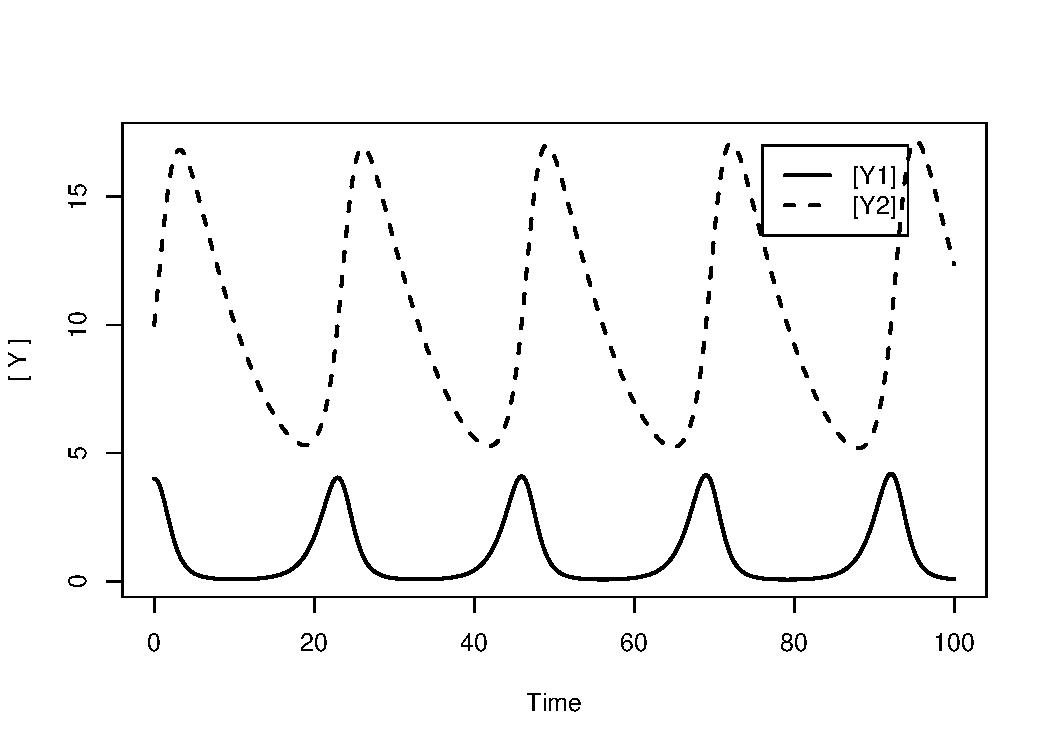
\includegraphics[width=5cm,clip=true]{figs/ch06-lv-dynamics}
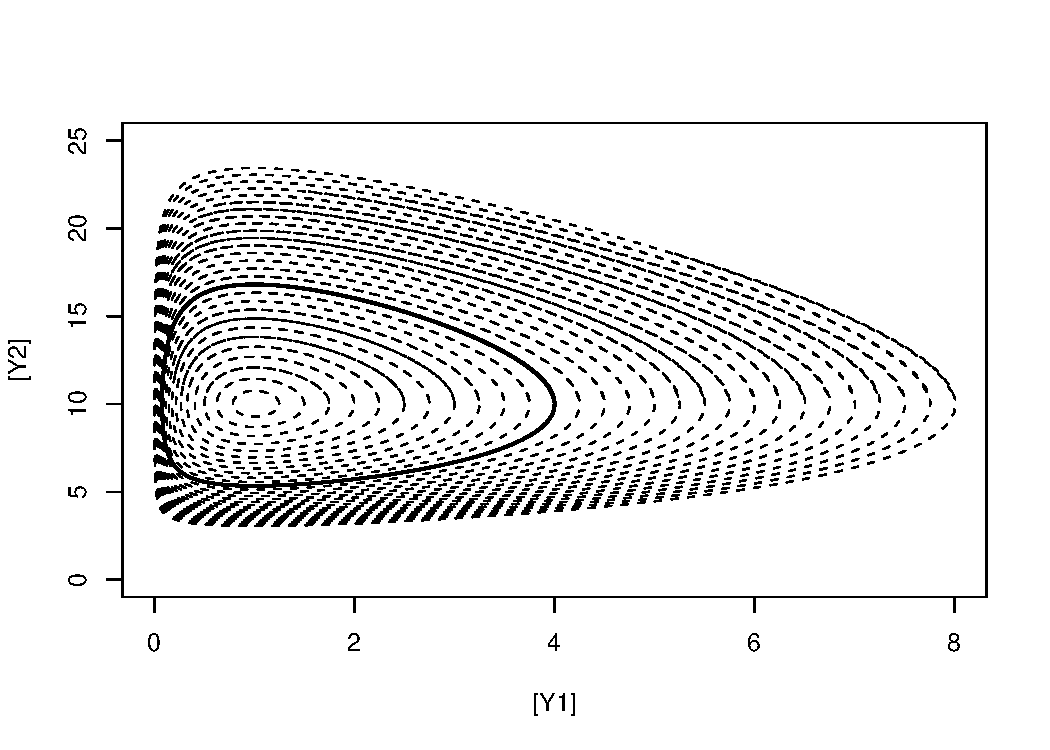
\includegraphics[width=5cm,clip=true]{figs/ch06-lv-phase}
\\
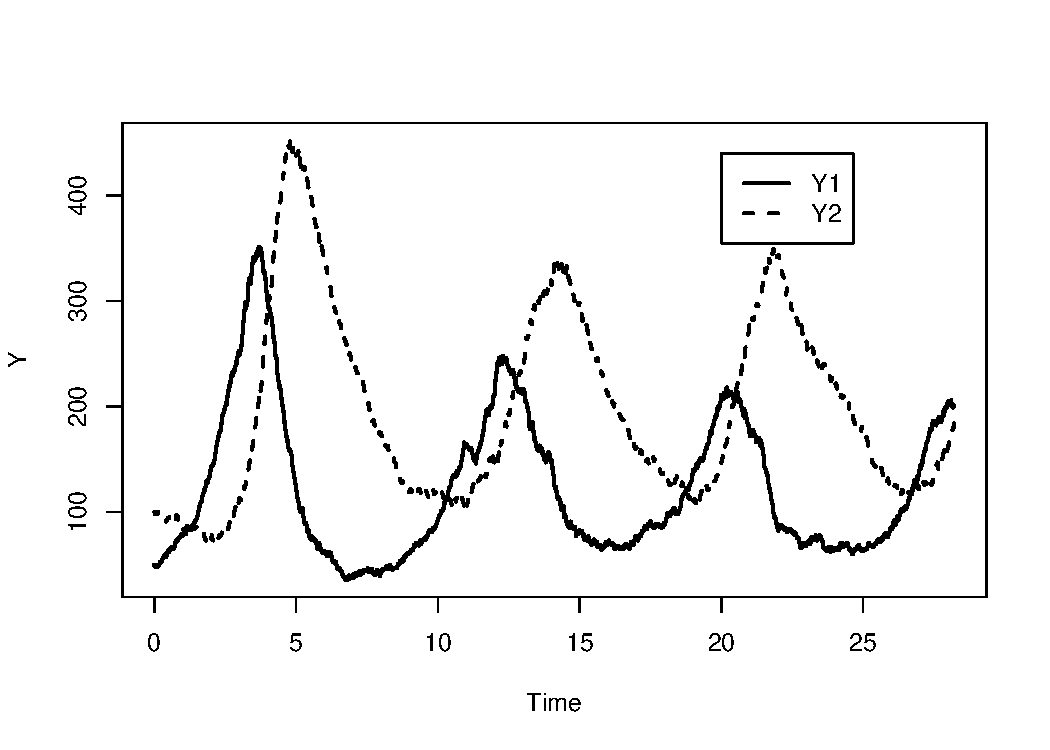
\includegraphics[width=5cm,clip=true]{figs/ch06-stoch-lv}
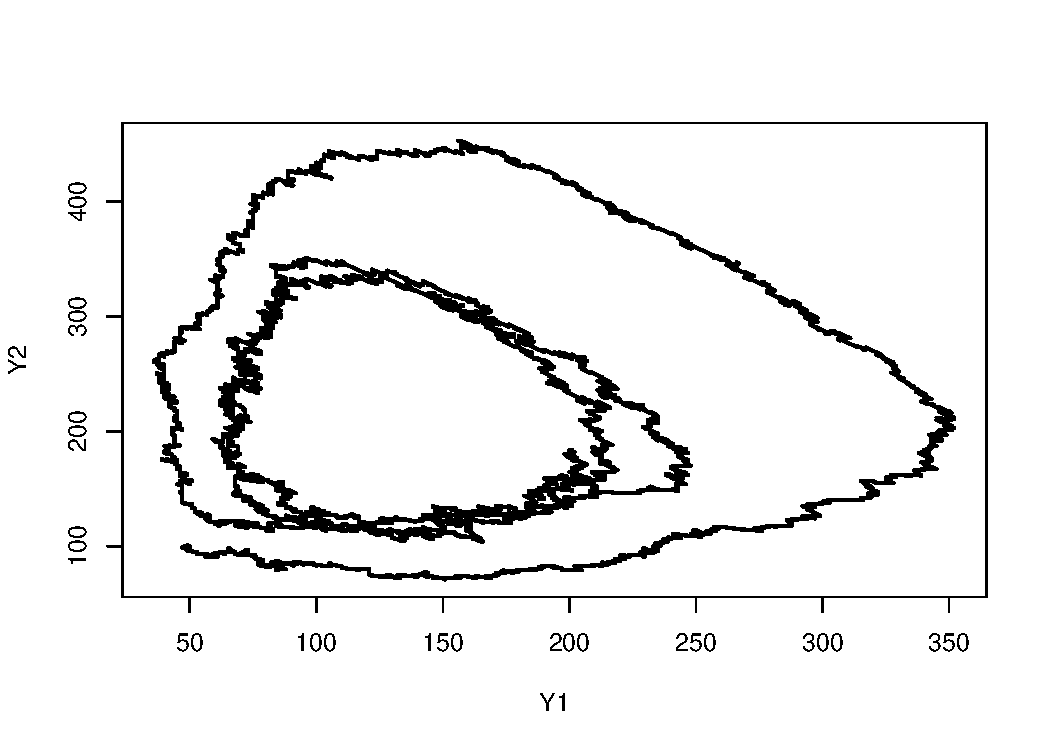
\includegraphics[width=5cm,clip=true]{figs/ch06-stoch-lv-phase}
}


\frame{
\frametitle{Key differences}
\begin{itemize}
\item Deterministic solution is exactly periodic with perfectly
repeating oscillations, carrying on indefinitely
\item Stochastic solution oscillates, but in a random, unpredictable
way (wandering from orbit to orbit in phase space)
\item Stochastic solution \alert{will} end in disaster! Either prey or
predator numbers will hit zero...
%\pause
\item Either way, predators will end up extinct, so \alert{expected}
number of predators will tend to zero --- \alert{qualitatively
different} to the deterministic solution
\item So, in general the deterministic solution does not provide
reliable information about either the stochastic process or its
average behaviour (and same is true of the LNA)
\end{itemize}
}



\frame{
\frametitle{Time change representation}
\begin{itemize}
\item $R_{it}$: \# reactions of type $\mathcal{R}_i$ in $(0,t]$, $R_t=(R_{1t},\ldots,R_{vt})'$
\item $X_t-X_0 = SR_t$ (state updating equation)
\item For $i=1,\ldots,v$, $N_i(t)$ are the count functions for
independent \alert{unit Poisson processes}, so
\[
R_{it}=N_i\left(\int_0^t h_i(X_{\tau},c_i)d\tau\right)
\]
\item Putting $N(t_1,\ldots,t_v)=(N_1(t_1),\ldots,N_v(t_v))'$, we can write
\(
R_t = N\left(\int_0^t h(X_{\tau},c)d\tau\right)\) to get:
\end{itemize}
\begin{block}{Time-change representation of the Markov jump process}
\centerline{\(\displaystyle
 X_t-X_0 = S\,N\left(\int_0^t h(X_{\tau},c)d\tau\right)
\)}
\end{block}
}



\frame{
\frametitle{Properties of the random time-change representation}
\begin{itemize}
\item The random time-change representation of a stochastic kinetic
model is due to \alert{Tom Kurtz}, and is a very useful and natural object for
mathematical analysis of stochastic kinetic models
\item In particular, it is good for understanding how algorithms for exact
  stochastic simulation, such as the \alert{Gillespie algorithm} and
  the Gibson-Bruck \alert{next reaction method} work 
\item It also provides the starting point for forming approximate
  models, such as diffusion approximations (chemical Langevin
  equation) and multi-scale approximations
\item It is more useful than the \alert{chemical Master equation} (Kolmogorov
forward equations) in many cases
\end{itemize}
}



\subsection{Stochasticity of p53 oscillations}


\frame{
\frametitle{Pathways to senescence}
\begin{itemize}
\item The mammalian group within CISBAN is interested in cell ageing
and many aspects of the processes which lead to cellular senescence,
and study this using immortalised human and rodent cell lines
\item \alert{DNA damage and repair processes} are one important component of
this large and complex system, and therefore molecules involved in
damage signalling and repair are of direct interest
\item Considerable interest in the role of \alert{p53} (``the guardian of the
genome'') in this context, and
the development of models for p53 regulation
\item p53 has many important functions, but of most relevance to this
discussion is its ability to \alert{activate DNA repair proteins} in response
to DNA damage
\end{itemize}
}

% \subsection{Experimental data}

\frame{
\frametitle{Single cell fluorescence microscopy}
\centerline{\includemovie[poster,text={Loading
movie...}]{0.8\textwidth}{0.8\textheight}{figs/p53-movie.mpg}}
}

\frame{
\frametitle{Single cell fluorescence microscopy}
\centerline{\includegraphics[height=0.7\textheight]{figs/p53image}}

\textcolor{green}{p53-CFP} and \textcolor{red}{Mdm2-YFP}\\
p53/Mdm2 oscillations subsequent to gamma irradiation
}


\frame{
\frametitle{Single cell time course data}
\centerline{\includegraphics[height=0.8\textheight]{figs/p53time}}
Geva-Zatorsky et al (2006), \emph{Mol.\ Sys.\ Bio.} [Uri Alon's lab]
}

%\subsection{Stochastic chemical kinetics}




%\subsection{Stochastic modelling of p53 oscillations}

\frame{
\frametitle{Stochastic kinetic model}
\begin{itemize}
\item \alert{Discrete stochastic kinetic model} developed at Newcastle 
(by \alert{Carole Proctor}) 
for the key biomolecular interactions between p53,
Mdm2 and their response to DNA damage induced by irradiation
\item More complex than a simple Lotka-Volterra system (17 species
and 20 reactions), but essentially the same regulatory
feedback mechanism (Mdm2 synthesis depends on the level of free p53, and
Mdm2 encourages degradation of p53)
\item
Some information about most kinetic parameters, but considerable
uncertainty for several --- ideal for a \alert{Bayesian analysis}
\end{itemize}
}

\frame{
\frametitle{Model structure and sample output}
\centerline{\includegraphics[width=1.1\textwidth]{figs/p53model-net}}
\centerline{
\includegraphics[height=0.5\textwidth,angle=90]{figs/p53-out1}
\includegraphics[height=0.5\textwidth,angle=90]{figs/p53-out2}
}
}


\section{Bayesian inference}

\subsection{Likelihood-free Bayesian inference}


\frame{
\frametitle{Bayesian inference}
Tuning model parameters so that output from the model ``better
matches'' experimental data is a standard optimisation problem, but is
problematic and unsatisfactory for a number of reasons:
\begin{itemize}
\item Defining an appropriate ``objective function'' is not
 straightforward if the model is stochastic or the measurement error
 has a complex structure (not IID Gaussian) 
\item The statistical
 concept of \alert{likelihood} provides the ``correct'' way of
 measuring the evidence in favour of a set of model parameters, but
 typically requires computationally intensive Monte Carlo procedures
 for evaluation in complex settings 
\item Simple optimisation of the
 likelihood (the \alert{maximum likelihood} approach) is also unsatisfactory,
 as there are typically many parameter combinations with very similar
 likelihoods (and the likelihood surface is typically multi-modal,
 making global optimisation difficult)
\end{itemize}
}

\frame{
\frametitle{Markov chain Monte Carlo (MCMC)}
\begin{itemize}
\item Additionally, likelihood ignores any existing information known
about likely parameter values \emph{a priori}, which can be very
useful for regularising the inference problem --- better to base
inference on the \alert{posterior distribution}
\item \alert{MCMC algorithms} can be used to explore plausible regions of
parameter space in accordance with the posterior distribution ---
these provide rich information
\item eg. rather than simple point estimates for parameter values, can get
\alert{plausible ranges} of values, together with information on parameter
\alert{identifiability} and \alert{confounding}
\item MCMC algorithms are computationally intensive, but given that
evaluation of the likelihood is typically computationally intensive
anyway, nothing to lose and everything to gain by doing a Bayesian
analysis
\end{itemize}
}

%\subsection{Likelihood for a stochastic kinetic model}


\frame{
\frametitle{Complete data likelihood}
\begin{itemize}
\item Observe process $\boldsymbol{x}=\{x(t):t\in[0,T]\}$
\item Time and type of $i$th reaction event is $(t_i,\nu_i)$,
$i=1,\ldots n$. Also define $t_0=0, t_{n+1}=T$
\item Let $r_i$ be the number of type $i$ events (so $n=\sum_{i=1}^n
r_i$)
\item The complete-data likelihood for the observed sample path is
\[
L(c;\boldsymbol{x})
= \left\{\prod_{i=1}^n 
 h_{\nu_i}(x(t_{i-1}),c_{\nu_i})
\right\}
\exp\left\{- \int_0^T h_0(x(t),c)\,dt 
\right\}
\]
(the integral is just a finite sum)
\item Complete-data likelihood is tractable, 
%though computationally
%  challenging, 
but we never completely observe the process
\end{itemize}
}


%\subsection{Partially observed Markov process (POMP) models}


\frame{
\frametitle{Partially observed Markov process (POMP) models}
\begin{itemize}
\item Continuous-time Markov process: $\mathbf{X}=\{X_s|s\geq 0\}$ (for now, we
  suppress dependence on parameters, $\theta$)
\item Think about integer time observations (extension to arbitrary
  times is trivial): for $t\in \mathbb{N},\quad
  \mathbf{X}_t=\{X_s|t-1<s\leq t\} $
\item Sample-path likelihoods such as $\pi(\mathbf{x}_t|x_{t-1})$ can
  often (but not always) be computed (but are often computationally
  difficult), but discrete time transitions such as $\pi(x_t|x_{t-1})$
  are typically intractable
\item Partial observations: $\mathcal{Y}=\{y_t|t=1,2,\ldots,T\}$ where
\[
y_t|X_t=x_t \sim \pi(y_t|x_t), \qquad t=1,\ldots,T,
\]
where we assume that $\pi(y_t|x_t)$ can be evaluated directly (simple
measurement error model)
\end{itemize}
}


\frame{
\frametitle{Bayesian inference for POMP models}
\begin{itemize}
\item Most ``obvious'' MCMC algorithms will attempt to impute (at
  least) the skeleton of the Markov process: $X_0,X_1,\ldots,X_T$
\item This will typically require evaluation of the intractable
  discrete time transition likelihoods, and this is the problem...
\item Two related strategies:
  \begin{itemize}
    \item \alert{Data augmentation}: ``fill in'' the entire process in
      some way, typically exploiting the fact that the sample path
      likelihoods are tractable --- works in principle, but difficult
      to ``automate'', and exceptionally computationally intensive due
      to the need to store and evaluate likelihoods of cts sample
      paths
    \item \alert{Likelihood-free} (AKA \alert{plug-and-play}): exploits the fact that it is
      possible to forward simulate from $\pi(x_t|x_{t-1})$ (typically
      by simulating from $\pi(\mathbf{x}_t|x_{t-1})$), even if it
      can't be evaluated
    \end{itemize}
\item Likelihood-free is really just a special kind of augmentation
  strategy
\end{itemize}
}



\frame{
\frametitle{``Likelihood-free'' MCMC}
\begin{itemize}
%\item Again
%$\pi(\mathcal{Y}|\mathbf{x})$ is a
%simple measurement error model...
\item Crucially, because the proposal exploits a forward simulation,
the acceptance probability does not depend on the likelihood of the
simulator output --- important for complex stochastic models
\item This scheme is completely general, and works very well provided
that $|\mathcal{Y}|$ is small
\item \alert{Problem:} If $|\mathcal{Y}|$ is large, the MCMC scheme
will mix very poorly (very low acceptance rates)
\item \alert{Solution:} Exploit the Markovian structure of the
process, and adopt a sequential approach, updating one
(or a small number of) observation(s) at a time...
\end{itemize}
}



\subsection{Inference for the p53 model}

\frame{
\frametitle{Parameter inference for the p53 model}
\centerline{\includegraphics[height=1.2\textheight,angle=270]{figs/M2all-parampost_bw}}
}

\frame{
\frametitle{Posterior correlations for the p53 model}
\centerline{\includegraphics[height=1.0\textheight,angle=270]{figs/M2all-paramcorr_bw}}
}

\frame{
\frametitle{Predictive fit for the p53 model}
\centerline{\includegraphics[height=1.2\textheight,angle=270]{figs/M2all-Zpred-p53_bw}}
}




\frame{
\frametitle{Advantages of the sequential algorithm}
\begin{itemize}
\item In the presence of measurement error, the sequential
likelihood-free scheme is effective, and is \alert{much} simpler than
a more efficient MCMC approach
\item The likelihood-free approach is easier to tailor to non-standard
models and data, and synthesis of data from multiple distinct models
with many shared parameters
\item The essential problem is that of \alert{calibration} of complex
stochastic computer models% --- \alert{paper by Goldstein}
% \item Worth connecting with the literature on deterministic computer
% models 
\item For \alert{slow} stochastic models, there is considerable
interest in developing fast \alert{emulators} and embedding these into
MCMC algorithms (as millions of forward-simulations from the model
will typically be required)% --- \alert{Daniel Henderson's poster}
\end{itemize}
}





\frame{
\frametitle{Limitations and alternatives}
\begin{itemize}
\item The LF-MCMC approach is simple and very general, but not without
problems
\item Scales badly as number of unknowns to be estimated increases
(curse of dimensionality) and as the number of sequential steps
increases (particle degeneracy)
\item Can we construct global and general MCMC
algorithms with better stability and numerical efficiency?
  \begin{itemize}
  \item \alert{Particle MCMC} one possibility --- more stable,
if not computationally cheaper (Andrieu et al, 2010)
  \item \alert{Diffusion approximation} --- approximate, but can then use
techniques of inference for SDE models (Golightly and W, '05, '06,
'08, '10, '11)
  \item \alert{Approximate MCMC} exploiting (semi-)tractable
stochastic emulators (Henderson et al, 2010)
  \item (Sequential) \alert{ABC} also possible --- but requires approximations, also not
cheap, and not trivial to automate (Toni et al, 2009)
  \end{itemize}
\end{itemize}
}





% \subsection{Software}

\frame{
\frametitle{R package: smfsb}
\begin{itemize}
\item Free, open source, well-documented software package for R on CRAN,
  \alert{\texttt{smfsb}}, associated with
  \alert{Stochastic modelling for systems biology, second edition}
\item Code for stochastic simulation and of (biochemical)
  reaction networks (Markov jump processes and chemical Langevin), and
  pMCMC-based Bayesian inference for POMP 
  models
\item Install with \alert{\texttt{install.packages("smfsb")}} and load with \alert{\texttt{library(smfsb)}} --- get a documentation overview with \alert{\texttt{help(package="smfsb")}}
\item Full installation and ``getting started'' instructions at \alert{\url{http://tinyurl.com/smfsb2e}}
\item Once the package is installed and loaded, running
  \alert{\texttt{demo("PMCMC")}} at the R prompt will run a PMMH
  algorithm %for the Lotka-Volterra model discussed here
\end{itemize}
}


\subsection{Limitations of likelihood-free approaches}

\frame{
\frametitle{Hitting the data...}
\begin{itemize}
\item The ``bootstrap'' PMMH algorithm works well in many cases, and is extremely
general (works for any Markov process)
\item In the case of no measurement error, the
probability of ``hitting'' the data (and accepting) is very
small (possibly zero), and so the mixing of the MCMC scheme is very poor
\item \alert{ABC} (approximate Bayesian computation) strategy is to accept if
\[
\Vert x_{t+1}^\star-y_{t+1}\Vert <\varepsilon
\]
but this forces a trade-off between accuracy and efficiency which can
be unpleasant (cf. \alert{noisy ABC})
\item Same problem in the case of low measurement error
\item Particularly problematic in the context of high-dimensional data
\item Would like a strategy which copes better in
this case
\end{itemize}
}


\frame{
\frametitle{The chemical Langevin equation (CLE)}
\begin{itemize}
\item The CLE is a diffusion approximation to the true Markov jump
process
\item Start with the time change representation
\[
X_t-X_0 = S\,N\left(\int_0^t h(X_{\tau},c)d\tau\right)
\]
and approximate $N_i(t)\simeq t+W_i(t)$, where $W_i(t)$ is an independent 
Wiener process for each $i$
\item Substituting in and using a little stochastic calculus gives:
\end{itemize}
\begin{block}{The CLE as an It\^o SDE:}
\centerline{\(\displaystyle
dX_t = Sh(X_t,c)\,dt + \sqrt{S\operatorname{diag}\{h(X_t,c)\}S'}\,dW_t
\)}
\end{block}
}

\subsection{Improved particle filters for SDEs}

\frame{
\frametitle{Improved particle filters for SDEs}
\begin{itemize}
\item The ``bootstrap'' particle filter uses blind forward simulation
  from the model
\item If we are able to evaluate the ``likelihood'' of sample paths,
  we can use other proposals
\item The particle filter weights then depend on the Radon-Nikodym
  derivative of law of the proposed path wrt the true conditioned
  process
\item For SDEs, the weight will degenerate unless the proposed process
  is absolutely continuous wrt the true conditioned process
\item Ideally we would like to sample from
  $\pi(\mathbf{x}_{t+1}^\star|c^\star,x_t^\star,y_{t+1})$, but this is
  not tractable for nonlinear SDEs such as the CLE --- instead sample
  from a tractable approximation (Golightly \& W, 2011)
\end{itemize}
}















\section{Inference for the structure of dynamic networks}

\subsection{High-throughput data}

\frame{
\frametitle{High throughput (HTP) data}
\begin{itemize}
\item Although we would prefer to use high-resolution single-cell time course
data for all of our statistical modelling, such data is difficult to
obtain in a high throughput (HTP) fashion for large numbers of proteins
\item
We therefore wish to integrate HTP data into our modelling
approach. Such data is usually of \alert{lower resolution} and possessing
relatively poor \alert{dynamic range}, but provides (simultaneous) measurement
of very large numbers of biological features
\item HTP data is potentially useful for uncovering network structure
\end{itemize}
}

\frame{
\frametitle{Time course microarray data}
\centerline{\includegraphics[height=0.9\textheight]{figs/ma-heat}}
}


\subsection{Sparse VAR(1) models}

\frame{
\frametitle{Sparse VAR(1) model}
\begin{itemize}
\item Observe a $p$-dimensional vector~$X_t$, at each of~$n$ time
points, $t=1,\ldots,n$ (with~$p>>n$)
\begin{align*}
X_{t+1} &= \mu + A(X_t-\mu) + \epsilon_t,\quad \epsilon_t\sim N(0,V)
\end{align*}
\item The $p\times p$ matrix $A$ is assumed to be \alert{sparse}
(ie. most elements are expected to be exactly zero)
\item Sparsity can be modelled in many ways. Simplest:
\[
\operatorname{Pr}(a_{ij}\not=0)=\pi,\ \forall i,j,\qquad
a_{ij}|a_{ij}\not=0\sim N(0,\sigma^2),\ \forall i,j
\]
\item The non-zero structure of $A$ can be associated with a
\alert{graph} (network) of 
\alert{dynamic interactions} (non-zero $a_{ij}$ implies arc from node $j$ to
node $i$)
\end{itemize}
}

\frame{
\frametitle{Inference for model parameters and structure from data}
\begin{itemize}
\item Can get a \alert{point estimate} for the
network structure by computing a \alert{shrinkage estimate} of $A$ and then
thresholding (Opgen-Rhein \& Strimmer, 2007)
\item Can also use \alert{Bayesian MCMC methods} to explore the space of
plausible interaction graphs
\item MCMC methods allow computation of useful quantities such as
$\operatorname{Pr}(a_{ij}\not=0|\mathcal{Y})$ 
\item Inference for graphs is a hard problem... \alert{(Lei et al, 2011)}
\end{itemize}
}

\frame{
\frametitle{MCMC for sparse VAR(1) models}
\begin{itemize}
\item \alert{RJ-MCMC algorithm} to explore both graphical structure and model
parameters (auto-regressive coefficients, mean vector, variance
components) --- routine to develop and implement, but exhibits
poor mixing in high-dimensional settings
\item Conditional on the graphical structure, possible (but messy) to
develop a \alert{variational algorithm} which gives an approximate marginal
log-likelihood for the model after a few iterations --- can embed this
in a very simple MCMC algorithm to explore just the graphical
structure
\item Even this algorithm \alert{mixes poorly} for large $p$ (say, $p>200$),
but there are $2^{p^2}$ graphs, after all...
\item Could probably get reasonable speed-up by using (parallel) \alert{sparse matrix algorithms}
\end{itemize}
}


\subsection{Application to yeast gene regulation}

\frame{
\frametitle{Connectivity matrix for the yeast data}
\centerline{\includegraphics[height=0.8\textheight]{figs/yeast-matrix}}

}

\frame{
\frametitle{Inferred network for the yeast data}
\vspace*{4ex}
\centerline{\includegraphics[width=\textwidth]{figs/yeast-network}}

}

\section{Summary and conclusion}

\subsection{Summary}

\frame{
\frametitle{Summary}
\begin{itemize}
\item Noise and heterogeneity are the norm in complex biological
  systems
\item Stochastic modelling provides a coherent framework for
  understanding sources of noise
\item Modern computationally intensive methods of statistical
  inference are useful for linking models to experimental data
\item Bayesian methods are especially useful and natural for fitting
  complex stochastic models to data
\item Detailed mechanistic models are appropriate for detailed
  single-cell data, but more descriptive statistical models are useful
  for high-throughput data
\end{itemize}
}




\frame{
\frametitle{Factorisation of the complete-data likelihood}
\begin{itemize}
\item For rate laws of the form $h_i(x,c_i)=c_ig(x)$ (true for
mass-action stochastic kinetic models), the complete-data likelihood
factorises as
\[
L(c;\boldsymbol{x}) = \prod_{j=1}^v L_j(c_j;\boldsymbol{x})
\]
where
\[
L_j(c_j;\boldsymbol{x}) = 
c_j^{r_j} 
\exp\left\{- c_j \int_0^T  g_j(x(t))\,dt 
\right\},\quad j=1,\ldots,v
\]
\end{itemize}
}

\frame{
\frametitle{Parameter estimation}
\begin{itemize}
\item
Factorisation leads to MLEs of the form
\[
\widehat{c_j} = r_j\bigg/ \int_0^T g_j(x(t))dt
\]
\item or can be combined with priors of the form $c_j\sim
\Gamma(a_j,b_j)$ to get full-conditionals
\[
c_j|\boldsymbol{x} \sim \Gamma\left(
a_j+r_j,b_j+\int_0^T g_j(x(t))dt
\right)
\]
\end{itemize}
}


\section{Bayesian network integration}

\frame{
\frametitle{Bayesian network integration}
\begin{itemize}
\item Networks are often inferred statistically using error prone
  techniques
\item Inferred networks will contain ``false positive'' edges which
  are present in the inferred network but
  should not be
\item They will also missing ``false negative'' edges which should be
  present in the inferred network but are not
\item Often different groups of researchers will publish an inferred
  network --- each network will be different
\item Reconciling these different networks to give a single concensus
  network with probabilistically scored edges is an interesting
  statistical inference problem 
\item Traditionally this was done by comparing the inferred networks
  against a ``gold standard'' in order to infer accuracy, but such
  gold standards rarely exist in practice \alert{(Weile et al, 2012)}
\end{itemize}
}


\subsection{Likelihood-free algorithms for stochastic model calibration}

\frame{
\frametitle{Bayesian inference}
\begin{itemize}
\item
Let $\pi(\mathbf{x}|c)$ denote the (complex) likelihood of
the \alert{simulation model}
\item
Let $\pi(\mathcal{Y}|\mathbf{x},\tau)$ denote
the (simple) measurement \alert{error model}
\item 
Put $\theta=(c,\tau)$,
and let $\pi(\theta)$ be the \alert{prior} for the model parameters
\item
The
\alert{joint} density can be written
\[
\pi(\theta,\mathbf{x},\mathcal{Y})=\pi(\theta)\pi(\mathbf{x}|\theta)\pi(\mathcal{Y}|\mathbf{x},\theta).
\]
\item
Interest is in the \alert{posterior} distribution
$\pi(\theta,\mathbf{x}|\mathcal{Y})$
\end{itemize}
}



\frame{
\frametitle{Marginal MH MCMC scheme}
\begin{itemize}
\item Full model: $\pi(\theta,\mathbf{x},\mathcal{Y}) = \pi(\theta)\pi(\mathbf{x}|\theta)\pi(\mathcal{Y}|\mathbf{x},\theta)$
\item Target: $\pi(\theta|\mathcal{Y})$ (with $\mathbf{x}$
  marginalised out)
%\item Specify a ``measurement error model'',
%$\pi(\mathcal{Y}|\mathbf{x},\theta)$ --- eg. just a product of Gaussian or t
%densities%, but could also integrate out a GASP 
%representing systematic error...
\item Generic MCMC scheme:
	\begin{itemize}
	\item Propose $\theta^\star \sim f(\theta^\star|\theta)$
	\item Accept with probability $\min\{1,A\}$, where
\[
A = \frac{\pi(\theta^\star)}{\pi(\theta)} \times
\frac{f(\theta|\theta^\star)}{f(\theta^\star|\theta)} \times \frac{\pi(\mathcal{Y}|\theta^\star)}{\pi(\mathcal{Y}|\theta)}
\]
	\end{itemize}
\item $\pi(\mathcal{Y}|\theta)$ is the ``marginal likelihood'' (or
``observed data likelihood'', or...)
\end{itemize}
}


\frame{
\frametitle{Special case: deterministic model}
\begin{itemize}
\item Deterministic function $g(\cdot)$ such that $\mathbf{x}=g(\theta)$
\item Then
\begin{align*}
\pi(\mathcal{Y}|\theta) &=
\pi(\mathcal{Y}|\theta,g(\theta)) \\ &=
\pi(\mathcal{Y}|\theta,\mathbf{x})
\end{align*}
\item Here $\pi(\mathcal{Y}|\theta,\mathbf{x})$ is just the ``measurement error model''
--- eg. simple product of Gaussian or $t$ densities
\item This setup is somewhat simplistic for the deterministic case, but
we are really more concerned with the stochastic case...
\end{itemize}
}



\frame{
\frametitle{LF-MCMC}
\begin{itemize}
\item
Posterior distribution
$\pi(\theta,\mathbf{x}|\mathcal{Y})$
\item Propose a joint update for $\theta$ and
$\mathbf{x}$ as follows: 
  \begin{itemize}
  \item Current state of the chain is $(\theta,\mathbf{x})$
  \item First sample $\theta^\star\sim f(\theta^\star|\theta)$
  \item Then sample a new path,
    $\mathbf{x}^\star\sim\pi(\mathbf{x}^\star|\theta^\star)$
  \item Accept the \alert{pair} $(\theta^\star,\mathbf{x}^\star)$ with probability
$\min\{1,A\}$, where
\[
A = \frac{\pi(\theta^\star)}{\pi(\theta)} \times
\frac{f(\theta|\theta^\star)}{f(\theta^\star|\theta)} \times \frac{\pi(\mathcal{Y}|\mathbf{x}^\star,\theta^\star)}{\pi(\mathcal{Y}|\mathbf{x},\theta)}.
\]
  \end{itemize}
\item
Note that choosing a \alert{prior independence proposal} of the form
$f(\theta^\star|\theta) = \pi(\theta^\star)$ leads to the simpler
acceptance ratio
\[
A =  \frac{\pi(\mathcal{Y}|\mathbf{x}^\star,\theta^\star)}{\pi(\mathcal{Y}|\mathbf{x},\theta)}
\]
\end{itemize}
}

\frame{
\frametitle{Sequential likelihood-free algorithm}
\begin{itemize}
\item Data $\mathcal{Y}_t=\{y_1,\ldots,y_t\}$,
$\mathcal{Y}\equiv\mathcal{Y}_n$. Sample paths
$\mathbf{x}_{t}\equiv\{x_s|t-1<s\leq t\}$, $t=2,3,\ldots,n$, so that
$\mathbf{x}\equiv\{\mathbf{x}_2,\ldots,\mathbf{x}_n\}.$
\end{itemize}
\begin{enumerate}
\item Assume at time $t$ we have a (large) sample from
$\pi(\theta,x_t|\mathcal{Y}_t)$ (for time 0, initialise with sample from prior)
\item Run an MCMC algorithm which constructs a proposal in two stages:
	\begin{enumerate}
	\item First sample
$(\theta^\star,x_t^\star)\sim\pi(\theta,x_t|\mathcal{Y}_t)$ by picking at random
and perturbing slightly (sampling from the kernel density estimate)
	\item Next sample $\mathbf{x}_{t+1}^\star$
by forward simulation from
$\pi(\mathbf{x}_{t+1}^\star|x_t^\star,\theta^\star)$
	\item Accept/reject $(\theta^\star,x_{t+1}^\star)$ with
\[
A=\frac{\pi(y_{t+1}|x_{t+1}^\star,\theta^\star)}{\pi(y_{t+1}|x_{t+1},\theta)}
\]
	\end{enumerate}
\item Output $\pi(\theta,x_{t+1}|\mathcal{Y}_{t+1})$, put $t:\,=t+1$, return to step 2.
\end{enumerate}
}


%\subsection{Particle MCMC and the PMMH algorithm}

\frame{
\frametitle{Particle MCMC (pMCMC)}
\begin{itemize}
\item Of the various alternatives, pMCMC is the only obvious practical
  option for constructing global likelihood-free MCMC algorithms which
  are exact (\alert{\href{http://dx.doi.org/10.1111/j.1467-9868.2009.00736.x}{Andrieu et al, 2010}})
\item Start by considering a basic marginal MH MCMC scheme with target
  $\pi(\theta|\mathcal{Y})$ and proposal $f(\theta^\star|\theta)$ ---
  the acceptance probability is $\min\{1,A\}$ where
\[
A = \frac{\pi(\theta^\star)}{\pi(\theta)}\times
\frac{f(\theta|\theta^\star)}{f(\theta^\star|\theta)}\times \frac{\pi(\mathcal{Y}|\theta^\star)}{\pi(\mathcal{Y}|\theta)}
\]
\item We can't evaluate the final terms, but if we had a way to
  construct a Monte Carlo estimate of the likelihood,
  $\hat\pi(\mathcal{Y}|\theta)$, we could just plug this in and hope
  for the best:
\[
A = \frac{\pi(\theta^\star)}{\pi(\theta)}\times
\frac{f(\theta|\theta^\star)}{f(\theta^\star|\theta)}\times \frac{\hat\pi(\mathcal{Y}|\theta^\star)}{\hat\pi(\mathcal{Y}|\theta)}
\]
\end{itemize}
}


\frame{
\frametitle{``Exact approximate'' MCMC (the pseudo-marginal approach)}
\begin{itemize}
\item
Remarkably, provided only that
$\operatorname{E}[\hat\pi(\mathcal{Y}|\theta)]=\pi(\mathcal{Y}|\theta)$,
the stationary distribution of the Markov chain will be
\alert{exactly} correct (\alert{\href{http://www.genetics.org/cgi/content/abstract/164/3/1139}{Beaumont, 2003}}, \alert{\href{http://dx.doi.org/10.1214/07-AOS574}{Andrieu \& Roberts, 2009}})
\item
Putting $W=\hat\pi(\mathcal{Y}|\theta)/\pi(\mathcal{Y}|\theta)$ and
augmenting the state space of the chain to include $W$, we find that
the target of the chain must be
\[
\propto \pi(\theta)\hat\pi(\mathcal{Y}|\theta)\pi(w|\theta) \propto
\pi(\theta|\mathcal{Y})w\pi(w|\theta)
\]
and so then the above ``unbiasedness'' property implies that
$\operatorname{E}(W|\theta)=1$, which
guarantees that the marginal for $\theta$ is exactly
$\pi(\theta|\mathcal{Y})$
%\item Blog post: \alert{\url{http://tinyurl.com/6ex4xqw}}
\end{itemize} 
}



%\subsection{PMMH}

\frame{
\frametitle{Particle marginal Metropolis-Hastings (PMMH)}
\begin{itemize}
\item Likelihood estimates constructed via importance sampling typically have
  this ``unbiasedness'' property, as do estimates constructed using a
  particle filter
\item If a particle filter is used to construct the Monte Carlo
  estimate of likelihood to plug in to the acceptance probability, we
  get (a simple version of) the particle Marginal Metropolis Hastings
  (PMMH) pMCMC algorithm
\item The full PMMH algorithm also uses the particle filter to
  construct a proposal for $\mathbf{x}$, and has target
  $\pi(\theta,\mathbf{x}|\mathcal{Y})$ --- not just
  $\pi(\theta|\mathcal{Y})$
\item The (bootstrap) particle filter relies only on the ability to
  forward simulate from the process, and hence the entire procedure is
  ``likelihood-free''
\end{itemize} 
% Blog post: \alert{\url{http://bit.ly/kvznmq}}
See \alert{Golightly and Wilkinson (2011)} for further details
}



\frame{
\frametitle{Example --- genetic auto-regulation}
%\includegraphics[width=12cm,clip=true]{figs/auto-reg}
\centerline{\includegraphics[width=8cm,clip=true]{figs/ch01-auto-reg}}
}

\frame{
\frametitle{Biochemical reactions}
Simplified view:
\begin{block}{Reactions}
\begin{tabular}{cl}
$g+P_2 \longleftrightarrow g\cdot P_2$ & Repression \\
$g \longrightarrow g+r$ & Transcription \\
$r \longrightarrow r+P$ & Translation \\
$2P \longleftrightarrow P_2$ & Dimerisation \\
$r \longrightarrow \emptyset$ & mRNA degradation\\
$P \longrightarrow \emptyset$ & Protein degradation
\end{tabular}
\end{block}
%\pause
%But these aren't as nice to look at as the picture...
}


\subsection{Petri nets}

\frame{
\frametitle{Petri net representation}
\centerline{\includegraphics[width=8cm,clip=true]{figs/ch02-petri}}
\vspace{0.5cm}
Simple bipartite digraph representation of the reaction
network --- useful both for visualisation and computational analysis
}

\frame{
\frametitle{Matrix representation of the Petri net}
\begin{center}
\small
\begin{tabular}{|r|ccccc|ccccc|}\cline{2-11}
\multicolumn{1}{c|}{ } & \multicolumn{5}{|c|}{Reactants ($Pre$)} &
\multicolumn{5}{|c|}{Products ($Post$)} \\ \hline
Species & $g\cdot P_2$ & $g$ & $r$ & $P$ & $P_2$ & $g\cdot P_2$ & $g$ & $r$ & $P$ & $P_2$ \\ \hline
Repression 		& &1& & &1&1& & & & \\
Reverse repression 	&1& & & & & &1& & &1\\
Transcription 		& &1& & & & &1&1& & \\
Translation 		& & &1& & & & &1&1& \\
Dimerisation 		& & & &2& & & & & &1\\
Dissociation 		& & & & &1& & & &2& \\
mRNA degradation	& & &1& & & & & & & \\
Protein degradation	& & & &1& & & & & & \\ \hline
\end{tabular}
\end{center}
% But still need rate laws and reaction rates...
Define $N=Post-Pre$ and $S=N'$, the \alert{stoichiometry matrix} of
the system
}



\subsection{Top-down models}


\frame{
\frametitle{The sparse VAR(1) model approximates the CLE}
\begin{itemize}
\item We have already seen how the true Markov jump process can be
approximated by the CLE
\item We can go further and \alert{linearise} the CLE to get a
multivariate Gaussian \alert{Ornstein-Uhlenbeck} (OU) process 
\item This OU process can be time-discretised exactly to give a VAR(1)
model with \alert{sparse} auto-regressive matrix (the sparsity of this
matrix derives from the sparsity of the stoichiometry matrix of the CLE)
\item This suggests that the sparse VAR(1) model might be a good
top-down model for
inferring the underlying structure of biochemical networks from
dynamic HTP data
\end{itemize}
}


\frame{
\frametitle{Simulated realisation of the auto-regulatory network}
\centerline{\includegraphics[height=9cm,clip=true,angle=90]{figs/ch07-ar-stochastic}}
}


%\subsection{Example: Lotka-Volterra model}

\frame{
\frametitle{Test problem: Lotka-Volterra model}
\centerline{\includegraphics[width=0.7\textwidth]{figs/ch10-LVnoise10}}

Simulated time series data set consisting of 16 equally spaced
  observations subject to Gaussian measurement error with a standard deviation
of 10.
}

\frame{
\frametitle{Marginal posteriors for the Lotka-Volterra model}
\centerline{\includegraphics[width=0.7\textwidth]{figs/ch10-LVboth}}

 Note that the true parameters, $\theta=(1,0.005,0.6)$
  are well identified by the data
}

\frame{
\frametitle{Marginal posteriors observing only prey}
\centerline{\includegraphics[width=0.7\textwidth]{figs/ch10-LVprey}}

Note that the mixing of the MCMC sampler is
  reasonable, and that the true parameters, $\theta=(1,0.005,0.6)$
  are quite well identified by the data
}



\frame{
\frametitle{The bootstrap particle filter}
\begin{itemize}
\item ``Particle cloud'': $\mathbf{x}_t=\{x_t^k|k=1,\ldots,M\}$,
  $\boldsymbol{\pi}_t=\{\pi_t^k|k=1,\ldots,M\}$,
  $\tilde{\mathbf{x}}_t=\{(x_t^k,\pi_t^k)|k=1,\ldots,M\}$
\item Initialise with $\tilde{\mathbf{x}}_0$, where $x_0^k\sim p(x_0)$ and
$\pi_0^k=1/M$ (note that $w_0^k$ is undefined)
\item Suppose at time $t$ we have a sample from
  $p(x_t|y_{1:t})$: $\tilde{\mathbf{x}}_t$
\begin{itemize}
\item Sample $a_t^k \sim \mathcal{F}(a_t^k|\boldsymbol{\pi}_t)$,
  $k=1,\ldots,M$
\item Sample $x_{t+1}^k\sim p(x_{t+1}^k|x_t^{a_t^k})$
\item Set $w_{t+1}^k=p(y_{t+1}|x_{t+1}^k)$ and
  $\pi_{t+1}^k=w_{t+1}^k/\sum_{i=1}^M w_{t+1}^i$
\item Propagate $\tilde{\mathbf{x}}_{t+1}$ to the next step...
\end{itemize}
\end{itemize}
Define $\hat{p}(y_t|y_{1:t-1})=\frac{1}{M}\sum_{i=1}^M w_t^i$ and
$\hat{p}(y_{1:T})=\prod_{i=1}^T \hat{p}(y_t|y_{1:t-1})$. Clear that
$\hat{p}(y_{1:T})$ is a \alert{consistent} estimator of $p(y_{1:T})$,
but not obvious that it is in fact also \alert{unbiased}
(\alert{Del Moral, 2004}, \alert{\href{http://arxiv.org/abs/1006.1914}{Pitt et al, 2011}}).

%Blog post: \alert{\url{http://bit.ly/jgo30P}}
}


\frame{
\frametitle{Marginal posteriors for unknown measurement error}
\centerline{\includegraphics[width=0.7\textwidth]{figs/ch10-LVsd}}

Note that the mixing of the MCMC sampler
  is poor, and that the true parameters, $\theta=(1,0.005,0.6,10)$ are
  less well identified by the data than in the case of a fully
  specified measurement error model
}

\section{Improved filtering proposals}

\subsection{Limitations of likelihood-free approaches}

\frame{
\frametitle{Hitting the data...}
\begin{itemize}
\item The ``bootstrap'' PMMH algorithm works well in many cases, and is extremely
general (works for any Markov process)
\item In the case of no measurement error, the
probability of ``hitting'' the data (and accepting) is very
small (possibly zero), and so the mixing of the MCMC scheme is very poor
\item \alert{ABC} (approximate Bayesian computation) strategy is to accept if
\[
\Vert x_{t+1}^\star-y_{t+1}\Vert <\varepsilon
\]
but this forces a trade-off between accuracy and efficiency which can
be unpleasant (cf. \alert{noisy ABC})
\item Same problem in the case of low measurement error
\item Particularly problematic in the context of high-dimensional data
\item Would like a strategy which copes better in
this case
\end{itemize}
}


\frame{
\frametitle{The chemical Langevin equation (CLE)}
\begin{itemize}
\item The CLE is a diffusion approximation to the true Markov jump
process
\item Start with the time change representation
\[
X_t-X_0 = S\,N\left(\int_0^t h(X_{\tau},c)d\tau\right)
\]
and approximate $N_i(t)\simeq t+W_i(t)$, where $W_i(t)$ is an independent 
Wiener process for each $i$
\item Substituting in and using a little stochastic calculus gives:
\end{itemize}
\begin{block}{The CLE as an It\^o SDE:}
\centerline{\(\displaystyle
dX_t = Sh(X_t,c)\,dt + \sqrt{S\operatorname{diag}\{h(X_t,c)\}S'}\,dW_t
\)}
\end{block}
}

\subsection{Improved particle filters for SDEs}

\frame{
\frametitle{Improved particle filters for SDEs}
\begin{itemize}
\item The ``bootstrap'' particle filter uses blind forward simulation
  from the model
\item If we are able to evaluate the ``likelihood'' of sample paths,
  we can use other proposals
\item The particle filter weights then depend on the Radon-Nikodym
  derivative of law of the proposed path wrt the true conditioned
  process
\item For SDEs, the weight will degenerate unless the proposed process
  is absolutely continuous wrt the true conditioned process
\item Ideally we would like to sample from
  $\pi(\mathbf{x}_{t+1}^\star|c^\star,x_t^\star,y_{t+1})$, but this is
  not tractable for nonlinear SDEs such as the CLE
\end{itemize}
}



\frame{
\frametitle{General SIR particle filter}
\begin{itemize}
\item At time $t$, we have (after resampling) an equally weighted sample from $\pi(x_t|y_{1:t})$
\item At time $t+1$, we want a weighted sample from $\pi(x_{t+1}|y_{1:t+1})$, though in fact useful to construct a sample from $\pi(x_{t+1},x_t|y_{1:t+1})$, and then marginalise down as required
\item Target $\propto \pi(y_{t+1}|x_{t+1})\pi(x_{t+1}|x_t)\pi(x_t|y_{1:t})$ and proposal is $f(x_{t+1}|x_t,y_{t+1})\pi(x_t|y_{1:t})$, for some $f(\cdot)$, leading to unnormalised weight
\[
w_{t+1}= \frac{\pi(y_{t+1}|x_{t+1})\pi(x_{t+1}|x_t)}{f(x_{t+1}|x_t,y_{t+1})}
\]
\item LF choice is $f(x_{t+1}|x_t,y_{t+1})=\pi(x_{t+1}|x_t)$, otherwise need to evaluate the discrete time transition density
\end{itemize}
}

\frame{
\frametitle{Weights and RN derivatives}
\begin{itemize}
\item For diffusions with intractable kernels, make the target $\pi(\mathbf{x}_{t+1},x_t|y_{1:t+1})$ and then marginalise down to $\pi(x_{t+1}|y_{1:t+1})$ if required
\item The proposal path will be of the form $f(\mathbf{x}_{t+1}|x_t,y_{t+1})\pi(x_t|y_{1:t})$, leading to weight
\[
w_{t+1} = \pi(y_{t+1}|x_{t+1})\frac{\pi(\mathbf{x}_{t+1}|x_t)}{f(\mathbf{x}_{t+1}|x_t,y_{t+1})}
\]
\item The expected weight is $\pi(y_{t+1}|y_{1:t})$, as needed for pseudo-marginal MCMC
\item Formally,
\[
w_{t+1}= \pi(y_{t+1}|x_{t+1})\frac{d\mathbb{P}}{d\mathbb{Q}}(\mathbf{x}_{t+1}|x_t),
\]
the RN derivative of the true (unconditioned) diffusion wrt the proposal process
\end{itemize}
}


\subsection{Approximate diffusion bridges}

\frame{
\frametitle{Modified diffusion bridge (MDB)}
\begin{itemize}
\item Need a tractable process
$q(\mathbf{x}_{t+1}^\star|c^\star,x_t^\star,y_{t+1})$ that is locally
equivalent to $\pi(\mathbf{x}_{t+1}^\star|c^\star,x_t^\star,y_{t+1})$
\item Diffusion $dX_t=\mu(X_t)dt+\beta(X_t)^\frac{1}{2}dW_t$
%\item For simplicity just consider the interval $[0,1]$, and suppose we
%are interested in the diffusion conditioned on both $X_0=x_0$ and
%$X_1=x_1$ (ie. perfect observation --- generalisations are
%straightforward)
%\item For the discrete derivation, consider an Euler-Maruyama
%discretisation with time step $\Delta t$ and increments
%\[
%(X_{t+\Delta t}|X_t=x_t) \sim N(x_t+\mu(x_t)\Delta t,\beta(x_t)\Delta t)
%\]
\item The nonlinear diffusion bridge on $[0,1]$
\[
dX_t = \frac{x_1-X_t}{1-t}dt + \beta(X_t)^\frac{1}{2}dW_t
\]
hits $x_1$ at $t=1$, yet is locally equivalent to the true conditioned diffusion
as it has the same diffusion coefficient
\item This forms the basis of an efficient proposal; see \alert{Durham \&
Gallant (2002)}, \alert{Chib, Pitt \& Shephard (2004)}, \alert{Delyon \& Hu (2006)},
and \alert{Stramer \& Yan (2007)} for technical details
\end{itemize}
}

\frame{
\frametitle{Discrete-time construction}
\begin{itemize}
\item Consider a forwards-simulation construction on $[0,1]$, and suppose that we  
have simulated as far as $t$
\item We know the distribution of the forward increment $X_{t+\Delta
t}$, but to condition on $x_1$ we would have to know $X_1|X_{t+\Delta
t}=x$
\item We use a very crude Euler-style approximation
\[
(X_1|X_{t+\Delta t}=x) \approxdist N(x+\mu(x_t)\Delta^+,\beta(x_t)\Delta^+)
\]
where $\Delta^+=1-t-\Delta t$
\item We now have a linear Gaussian structure, so can directly
condition to get
\[
(X_{t+\Delta t}|X_t=x_t,X_1=x_1) \approxdist N\left(
\frac{\Delta^+x_t+x_1\Delta t}{1-t} ,
\frac{\Delta^+}{1-t}\beta(x_t)\Delta t  \right)
\]
\end{itemize}
}

\frame{
\frametitle{MDB for partial observation}
\begin{itemize}
\item If we assume a Gaussian partial observation regime of the form
\[
Y_t = F' X_t + \eps_t, \quad \eps\sim N(0,\Sigma)
\]
we want to simulate from a bridge approximating $\pi(\mathbf{x}|x_0,y_1)$
\item We can extend the previous crude approximation to obtain
\[
(Y_1|X_{t+\Delta t}=x) \approxdist N( F'(x+\mu(x_t)\Delta^+),F'\beta(x_t)F\Delta^+ + \Sigma)
\]
\item This again gives a linear Gaussian structure enabling sequential conditional simulation of an approximating process
\end{itemize}
}

\frame{
\frametitle{Example: Efficient pMCMC for SDEs}
\begin{itemize}
\item Example from \alert{Golightly and W (2011)}
\item Inference for an auto-regulatory stochastic kinetic network model
\item Compare:
	\begin{itemize}
	\item Bootstrap PMMH with exact forward simulation
	\item Bootstrap PMMH with forward simulation from CLE approx
	\item PMMH with MDB filtering for CLE approx
	\end{itemize}
\item Look at marginals and ACFs for the 6 (out of 8) well identified parameters (other 2 partially confounded)
\end{itemize}
}

\frame{
\frametitle{Marginal posteriors for the auto-regulatory network}
\centerline{\includegraphics[width=0.7\textwidth]{figs/post1}}
\centerline{\includegraphics[width=0.7\textwidth]{figs/post2}}

}

\frame{
\frametitle{ACFs for the auto-regulatory network}
\centerline{\includegraphics[width=0.7\textwidth]{figs/acf1}}
\centerline{\includegraphics[width=0.7\textwidth]{figs/acf2}}
}



\section{Summary and conclusions}

\subsection{Summary}

\frame{
\frametitle{Summary}
\begin{itemize}
\item Exact LF MCMC inference is possible for intractable nonlinear Markov processes, provided that there is sufficient noise in the observation process
\item In low/no noise scenarios, efficient MCMC algorithms are still
  possible --- one approach is to use tractable bridging processes as proposals in an SMC-within-MCMC algorithm
\item This is one approach, but there are many others --- exact and approximate
\item The relative merits of the various possible approaches are currently poorly understood
\end{itemize}
}




\subsection{Markov jump process bridges}

\frame{
\frametitle{Markov jump process bridges}
\begin{itemize}
\item Simulate bridge over the interval $[0,s]$, conditional on $x(0)$ and
some observation $y$, where $Y=F' X(s)+\eps$, $\eps\sim
N(0,\Sigma)$
\item Suppose we have simulated as far as time $t$ to get $x(t)$, and
  wish to simulate next event
\item Put $\Delta t=s-t$, $\Delta X=X(s)-x(t)$, and $\Delta
  R=R_s-r_t$, so that $\Delta X = S\Delta R$
\item The unconditional hazard vector is $h(x(t))$, so a very crude
  approx for $\Delta R$ is 
\[\Delta R \approxdist Po(h(x(t))\Delta t) \approxdist
  N(h(x(t))\Delta t,\operatorname{diag}\{h(x(t))\}\Delta t)
\]
\item Under this approximation, $\Delta R$, $X(s)$ and $Y$ are jointly MVN,
  and so we can compute the conditional distribution $\Delta R|Y$
\end{itemize}
}


\frame{
\frametitle{Conditional hazard}
\begin{itemize}
\item
Conditioning gives
\begin{multline*}
\operatorname{E}(\Delta R|y) = h(x(t))\Delta t +
\operatorname{diag}\{h(x(t))\}G'\\
\times[\Sigma+G\operatorname{diag}\{h(x(t))\}G'\Delta
t]^{-1}\\ \times(y-F' x(t)-Gh(x(t))\Delta t)\Delta t
\end{multline*}
where $G=F' S$
\item Dividing through by $\Delta t$ gives a corresponding conditional
  hazard as
\begin{multline*}
h^\star(x(t)|y) = h(x(t)) +
\operatorname{diag}\{h(x(t))\}G'\\
\times[\Sigma+G\operatorname{diag}\{h(x(t))\}G'\Delta
t]^{-1}\\ \times(y-F' x(t)-Gh(x(t))\Delta t)
\end{multline*}
\end{itemize}
}

\frame{
\frametitle{Noiseless measurement}
\begin{itemize}
\item In the special case $\Sigma=0$ we have
\begin{multline*}
h^\star(x(t)|y) = h(x(t)) +
\operatorname{diag}\{h(x(t))\}G'
[G\operatorname{diag}\{h(x(t))\}G']^{-1}\\
\times\left(\frac{y-F' x(t)}{s- t}-Gh(x(t))\right)
\end{multline*}
\item This simplifies using the QR--factorisation of
  $\operatorname{diag}\{\sqrt{h(x(t))}\}G'$ to
\[
 h(x(t)) +
\operatorname{diag}\{\sqrt{h(x(t))}\}QR^{-\prime}
\left(\frac{y-F' x(t)}{s- t}-Gh(x(t))\right)
\]
\end{itemize}
}

\frame{
\frametitle{Lotka--Volterra example}
\begin{itemize}
\item Try out with the LV model, using noiseless observation of the prey only
\[
\hspace*{-2ex}
h=\begin{pmatrix}cx_1\\cx_1x_2\\c_3x_2\end{pmatrix},\ S=\begin{pmatrix}1&-1&0\\0&1&-1\end{pmatrix},\ F=\begin{pmatrix}1\\0\end{pmatrix},\ G=\begin{pmatrix}1&-1&0\end{pmatrix}
\]
\item
\[
h^\star = \begin{pmatrix}h_1\\h_2\\h_3\end{pmatrix} + \frac{1}{h_1+h_2}\left(\frac{y-x_{t1}}{s-t}-h_1+h_2\right)\begin{pmatrix}h_1\\-h_2\\0\end{pmatrix}
\]
\item Approximate implementation with exponential waiting times
\end{itemize}
}

\frame{
\frametitle{Good interval}
\centerline{\includegraphics[width=0.9\textwidth]{figs/int1b}}

}


\frame{
\frametitle{Bad interval}
\centerline{\includegraphics[width=0.9\textwidth]{figs/int2}}

}



%\subsection{The chemical Langevin equation}

\frame{
\frametitle{The Chemical Langevin Equation (CLE)}
\begin{itemize}
\item The CLE is just a \alert{diffusion approximation} for the Markov
Jump Process (MJP) derived from stochastic chemical kinetic theory
\item It is the It\^o \alert{stochastic differential equation} (SDE) model 
which ``most closely matches'' the dynamics of the MJP
\item Formally, it is constructed by first considering a second-order
approximation to the Kolmogorov forward equations for the process ---
known in this context as the \alert{Chemical Master Equation} (CME)
\item This second-order approximation is known as the \alert{Fokker-Planck
equation}, and is the Kolmogorov forward equation associated with the CLE
\end{itemize}
}





\frame{
\frametitle{Systems Biology models}
\begin{itemize}
\item Typically consist of a list of (bio-)chemical reactions, together with associated rate equations which
govern their ``speed''
\item The rate equations are usually a function of the current system state, as well as parameters (rate
constants)
\item From this, we need to make some assumptions about the nature of the kinetics, then end up with a
stochastic or deterministic kinetic model
\end{itemize}
}






\subsection{Introduction}




% \subsection{Bayesian inference}


\section{Case study: \protect\emph{B. subtilis} motility regulation}

\subsection{Introduction}

% \subsection{Stochastic modelling}

\frame{
\frametitle{\emph{Bacillus subtilis}}
\begin{itemize}
\item \emph{Bacillus subtilis} is the most widely studied model gram
  positive bacterium
\item It is easy to culture and highly genetically tractable
  (naturally competent for transformation)
\item Relatively interesting life cycle --- must make some expensive
  \alert{cellular decisions}
\item Can \alert{grow and divide}, become \alert{competent},
  \alert{sporulate}, or become \alert{motile}
\item The motility regulation network is large and complex --- for
  illustrative purposes, just focus on one aspect --- repression of
  \emph{fla/che} by \emph{CodY}
\end{itemize}
}

%\subsection{Motility regulation}

\frame{
\frametitle{Motility regulation}
\begin{itemize}
\item The $\sigma$ factor $\sigma^D$ (\emph{SigD}) is key to the
  regulation of motility --- many genes and operons encoding motility
  related proteins are governed by this $\sigma$ factor
\item \emph{hag} (encoding \emph{flagellin}) is one gene with a
  $\sigma^D$ promoter
\item \emph{sigD} is embedded in a large operon --- the \emph{fla/che}
  operon
\item \emph{fla/che} strongly repressed by \emph{CodY}, and
  \emph{CodY} is up-regulated in good nutrient conditions
\end{itemize}
\vspace{-2cm}

\centerline{\includegraphics[height=4cm]{figs/motility}}
}

%\section{Stochastic kinetic models}

%\subsection{Stochasticity in bacterial decisions}

\frame{
\frametitle{Stochasticity in bacterial decision making}
\begin{itemize}
\item Cellular processes are not deterministic, and the motility
  decision is no exception
\item There is considerable cell to cell variability in motility
  onset, even for isogenic batch cultures
\item Even in good nutrient conditions, a small fraction of cells will
  turn on motility function, and this is possibly evolutionarily
  beneficial (bet-hedging)
\item Although there are many other sources of heterogeneity,
  \alert{intrinsic stochasticity} in gene expression is of fundamental
  importance to understanding and modelling this process
\end{itemize}
}



%\subsection{Motility model}


\frame{
\frametitle{Motility model}
%%% START Reactions
{\small
\begin{align*}
\mathsf{codY} &\longrightarrow \mathsf{codY}+\mathsf{CodY}\\
\mathsf{CodY} &\longrightarrow  \emptyset \\
\mathsf{flache} &\longrightarrow \mathsf{flache}+\mathsf{SigD} \\
\mathsf{SigD} &\longrightarrow \emptyset\\
\mathsf{SigD\_hag} &\longrightarrow
\mathsf{SigD}+\mathsf{hag}+\mathsf{Hag}\\
\mathsf{Hag} &\longrightarrow  \emptyset\\
\mathsf{SigD}+\mathsf{hag} &\longrightarrow \mathsf{SigD\_hag} \\
\mathsf{SigD\_hag} &\longrightarrow \mathsf{SigD}+\mathsf{hag} \\
\mathsf{CodY}+\mathsf{flache} &\longrightarrow \mathsf{CodY\_flache}
\\
\mathsf{CodY\_flache} &\longrightarrow \mathsf{CodY}+\mathsf{flache}
\\
\mathsf{CodY}+\mathsf{hag} &\longrightarrow \mathsf{CodY\_hag} \\
\mathsf{CodY\_hag} &\longrightarrow \mathsf{CodY}+\mathsf{hag} \\
\end{align*}
}
%%% END Reactions
}



\frame{
\frametitle{Sample model trajectory}
\centerline{\includegraphics[angle=270,width=10cm]{figs/trajectory}}
}

\subsection{Inference for the motility model}


\frame{
\frametitle{Simulation study}
\begin{itemize}
\item 3 ``unknowns''
\item True values:\\
\medskip
 \(
kSigDprod=1,\ kflacherep=0.02,\ 
kflacheunrep=0.1
\) \\
\medskip
They correspond to the maximal rate of production of \textsf{SigD}, and the
binding and unbinding of \textsf{CodY} to the fla/che operon
\item Prior distributions: 
\begin{align*}
\log(kSigDprod) &\sim \operatorname{Unif}(\log\{0.01\},\log\{100\}) \\
\log(kflacherep) &\sim \operatorname{Unif}(\log\{0.0002\},\log\{2\}) \\
\log(kflacheunrep) &\sim \operatorname{Unif}(\log\{0.001\},\log\{10\})
\end{align*}
These priors cover two orders of magnitude either side of the true
value, and hence represent very vague prior knowledge
\end{itemize}
}

\subsection{Direct observation of protein levels}

\frame{
\frametitle{Observation of $\sigma^D$}
\begin{itemize}
\item Observe levels of $\sigma^D$ every 5 minutes for 2 hours (24
  observations) subject to low measurement error (standard deviation
  10 molecules)
\end{itemize}
\centerline{\includegraphics[angle=270,width=10cm]{figs/sigd-post}}
}

\frame{
\frametitle{Observation of $\sigma^D$}
\vspace{-0.8cm}
\centerline{\includegraphics[angle=270,width=10cm]{figs/sigd-cont}}
\vspace{-1.2cm}
\centerline{\includegraphics[angle=270,width=10cm]{figs/sigd-pred}}
}


\frame{
\frametitle{Observation of \emph{Hag}}
\begin{itemize}
\item $\sigma^D$ turns out to be difficult to measure directly ---
  what if we could measure \emph{Hag} instead?
\end{itemize}
\centerline{\includegraphics[angle=270,width=10cm]{figs/hag-post}}
}

\frame{
\frametitle{Observation of \emph{Hag}}
\vspace{-0.8cm}
\centerline{\includegraphics[angle=270,width=10cm]{figs/hag-cont}}
\vspace{-1.2cm}
\centerline{\includegraphics[angle=270,width=10cm]{figs/hag-pred}}
}


\subsection{Indirect observation via reporter proteins}

\frame{
\frametitle{GFP reporters}
\begin{itemize}
\item In fact, it is not straightforward to measure \alert{any}
 native protein directly --- instead \alert{reporters} are used
\item Example: Green fluorescent protein --- \emph{GFP}
\item The gene for \emph{GFP}, \emph{gfp} has to be integrated into
  the host genome in such a way as to try and make the levels of
  mature GFP correlate strongly with the levels of the target protein
  of interest --- not straightforward...
\item For $\sigma^D$, standard approach is to form a fusion of the
  \emph{hag} promoter, $P_{hag}$ to \emph{gfp} to get
  $P_{hag}$--\emph{gfp} and then integrate this construct at a
  convenient location in the genome, which is often at \emph{amyE}
\item Genotype of resulting mutant written:
  \emph{amyE}::$P_{hag}$--\emph{gfp}
\end{itemize}
}


% \begin{comment}

\frame{
\frametitle{Fluorescence microscopy for \emph{amyE}::$P_{hag}$--\emph{gfp}}
\centerline{\includemovie[poster,text={Loading
movie...}]{0.8\textwidth}{0.8\textheight}{figs/Movie-3.mpg}}
}

% \end{comment}

\frame{
\frametitle{GFP data}
\centerline{\includegraphics[height=6cm]{figs/Montage-3}}
}

\frame{
\frametitle{GFP Model}
\begin{itemize}
\item The additional species and reactions can be incorporated into the
  model and this shows the relationship of \emph{GFP} to the other model
  species
\end{itemize}
\vspace{-1cm}
\centerline{\includegraphics[angle=270,width=10cm]{figs/gfptraj}}
}




\frame{
\frametitle{Observation of \emph{GFP}}
\begin{itemize}
\item Observe levels of \emph{GFP} every 5 minutes for 2 hours (24
  observations) subject to low measurement error (standard deviation
  10 molecules)
%\item Now consider the observation of \emph{GFP} subject to small
%  measurement error
\end{itemize}
\centerline{\includegraphics[angle=270,width=10cm]{figs/gfp-post}}
}

\frame{
\frametitle{Observation of \emph{GFP}}
\vspace{-0.8cm}
\centerline{\includegraphics[angle=270,width=10cm]{figs/gfp-cont}}
\vspace{-1.2cm}
\centerline{\includegraphics[angle=270,width=10cm]{figs/gfp-pred}}
}



\frame{
\frametitle{Confusion of \emph{GFP} with $\sigma^D$}
\begin{itemize}
\item Now consider what happens when we observe \emph{GFP} subject to small
  measurement error but enter these measurements into the inference
  algorithm as $\sigma^D$
\end{itemize}
\centerline{\includegraphics[angle=270,width=10cm]{figs/gfp-sigd-post}}
}

\frame{
\frametitle{Confusion of \emph{GFP} with $\sigma^D$}
\vspace{-0.8cm}
\centerline{\includegraphics[angle=270,width=10cm]{figs/gfp-sigd-cont}}
\vspace{-1.2cm}
\centerline{\includegraphics[angle=270,width=10cm]{figs/gfp-sigd-pred}}
}


\section{``Exact approximate'' MCMC and Particle MCMC}

\subsection{The pseudo-marginal approach}

\frame{
\frametitle{``Ideal'' joint MCMC scheme}
\begin{itemize}
\item LF-MCMC works by making the proposed sample path consistent with
  the proposed new parameters, but unfortunately not with the data
\item Ideally, we would do the joint update as follows
  \begin{itemize}
  \item First sample $\theta^\star\sim f(\theta^\star|\theta)$
  \item Then sample a new path,
    $\mathbf{x}^\star\sim\pi(\mathbf{x}^\star|\theta^\star,\mathcal{Y})$
  \item Accept the \alert{pair} $(\theta^\star,\mathbf{x}^\star)$ with probability
$\min\{1,A\}$, where
\begin{align*}
A &= \frac{\pi(\theta^\star)}{\pi(\theta)} 
\frac{\pi(\mathbf{x}^\star|\theta^\star)}{\pi(\mathbf{x}|\theta)} 
\frac{f(\theta|\theta^\star)}{f(\theta^\star|\theta)} 
\frac{\pi(\mathcal{Y}|\mathbf{x}^\star,\theta^\star)}{\pi(\mathcal{Y}|\mathbf{x},\theta)}
\frac{\pi(\mathbf{x}|\mathcal{Y},\theta)}{\pi(\mathbf{x}^\star|\mathcal{Y},\theta^\star)}\\
&= \frac{\pi(\theta^\star)}{\pi(\theta)}
\frac{\pi(\mathcal{Y}|\theta^\star)}{\pi(\mathcal{Y}|\theta)} \frac{f(\theta|\theta^\star)}{f(\theta^\star|\theta)}
\end{align*}
\item This joint scheme reduces down to the marginal scheme
  (\alert{\href{http://www.jstor.org/stable/2291521}{Chib (1995)}}), but will
  be intractable for complex models...
  \end{itemize}
\end{itemize}
}

\frame{
\frametitle{Why the pseudo-marginal idea is important}
\begin{itemize}
\item Many MCMC algorithms suffer from slow convergence due to high
  dependence between parameters, or between parameters and ``missing
  data''
\item In principle it is possible to greatly improve the rate of
  convergence by ``integrating out'' or marginalising over parameters
  not of direct inferential interest
\item Marginalising over parameters or missing data leads to the
  occurrence of (often intractable) marginal likelihood terms in MCMC
  algorithms
\item The pseudo-marginal approach gives the possibility of developing
  exact MCMC algorithms using approximate (unbiased, Monte Carlo)
  estimates of marginal likelihoods
\item There are several well-known methods for constructing unbiased
  estimates of marginal likelihood
\end{itemize}
}


\frame{
\frametitle{Particles and genealogies}
\centerline{\includegraphics[height=0.8\textheight]{figs/smc}}
\noindent Figure from
\alert{\href{http://dx.doi.org/10.1111/j.1467-9868.2009.00736.x}{Andrieu
    et al (2010)}}
}

\frame{ 
\frametitle{Joint density}
It is important to know the full joint density of all random variables
generated by the particle filter, which we write as
\[
\tilde{q}(\mathbf{x}_0,\ldots,\mathbf{x}_T,\mathbf{a}_0,\ldots,\mathbf{a}_{T-1})
= \left[\prod_{k=1}^M p(x_0^k)\right] \left[\prod_{t=0}^{T-1}
  \prod_{k=1}^M \pi_t^{a_t^k} p(x_{t+1}^k|x_t^{a_t^k}) \right]
\]
on $X^{M(T+1)}\times\{1:M\}^{MT}$. For PMMH we also sample a final index
$k'$ from $\mathcal{F}(k'|\boldsymbol{\pi}_T)$ giving the joint
density 
\[
\tilde{q}(\mathbf{x}_0,\ldots,\mathbf{x}_T,\mathbf{a}_0,\ldots,\mathbf{a}_{T-1})\pi_T^{k'}
\]
on $X^{M(T+1)}\times\{1:M\}^{MT+1}$. We write the final selected
trajectory as
\[
x_{0:T}^{k'}=(x_0^{b_0^k},\ldots,x_T^{b_T^{k'}}),
\]
where $b_t^{k'}=a_t^{b_{t+1}^{k'}}$, and $b_T^{k'}=k'$.
}

\subsection{The PMMH algorithm}

\frame{
\frametitle{PMMH algorithm}
\begin{itemize}
\item Propose $\theta^\star \sim q(\theta^\star|\theta)$
\item Sample $\mathbf{x}_{0:T}^\star$ by running a bootstrap particle
  filter and picking a trajectory using the final set of weights,
  $\boldsymbol{\pi}_T$
\item Evaluate the estimate of marginal likelihood of the data, $\hat{p}_{\theta^\star}(y_{1:T})$
\item Accept proposed new values with ratio
\[
A = \frac{\hat{p}_{\theta^\star}(y_{1:T})p(\theta^\star)q(\theta|\theta^\star)}{\hat{p}_{\theta}(y_{1:T})p(\theta)q(\theta^\star|\theta)}
\]
\item On the fully augmented space $(\Theta\times
  X^{M(T+1)}\times\{1:M\}^{MT+1})$, the proposal is
\[
q(\theta^\star|\theta)\tilde{q}_{\theta^\star}(\mathbf{x}_0^\star,\ldots,\mathbf{x}_T^\star,\mathbf{a}_0^\star,\ldots,\mathbf{a}_{T-1}^\star)\pi_T^{{k'}^\star}
\]
\end{itemize}
}


\frame{
\frametitle{PMMH augmented target}
\begin{itemize}
\item By considering the proposal and the acceptance ratio, it is
  clear that the augmented target must be proportional to
\[
p(\theta)\hat{p}_\theta(y_{1:T})
\tilde{q}_\theta(\mathbf{x}_0,\ldots,\mathbf{x}_T,\mathbf{a}_0,\ldots,\mathbf{a}_{T-1})
\pi_T^{k'}
\]
\item We want to show that when we marginalise this down to the
  accepted trajectory, it is proportional to
  $p(\theta,x_{0:T}|y_{1:T})$
\item Consider the terms  in the joint distribution of the particle
  filter random variables
\[
\tilde{q}_\theta(\mathbf{x}_0,\ldots,\mathbf{x}_T,\mathbf{a}_0,\ldots,\mathbf{a}_{T-1})
\pi_T^{k'}
\]
corresponding to the trajectory selected by final index $k'$,
\[
x_{0:T}^{k'} = (x_0^{b_0^{k'}},\ldots,x_T^{b_T^{k'}})
\]
\end{itemize}
}

\frame{
\frametitle{Likelihood of selected trajectory}
\begin{itemize}
\item This is given by
\[
p_\theta(x_0^{b_0^{k'}})\left[\prod_{t=0}^{T-1} \pi_t^{b_t^{k'}}
  p_\theta(x_{t+1}^{b_{t+1}^{k'}}|x_t^{b_t^{k'}})\right]\pi_T^{k'}
=
p_\theta(x_{0:T}^{k'})\prod_{t=0}^T \pi_t^{b_t^{k'}}
\]
\item This probability simplifies to
\[
\frac{p_\theta(x_{0:T}^{k'})p_\theta(y_{1:T}|x_{0:T}^{k'})}{M^{T+1}\hat{p}_\theta(y_{1:T})}
\]
\item \alert{This} is why PMMH works!
\end{itemize}
}

\frame{
\frametitle{The selected trajectory and the target}
\begin{itemize}
\item Consequently, the normalising constant cancels and the target is
  (proportional to)
\[
\frac{p(\theta)p_\theta(x_{0:T}^{k'},y_{1:T})}{M^{T+1}} \times
\text{(Other terms...)}
\]
\item The other terms are all probabilities of random variables which
  do not occur elsewhere in the target, and hence can all be
  marginalised away to leave the correct posterior
\[
p(\theta,x_{0:T}|y_{1:T})
\]
(also note the uniform distribution on the selected indices)
\end{itemize}
Blog post: \alert{\url{http://bit.ly/kvznmq}}
}


\begin{frame}[fragile]
  This can be
encoded in R as a stochastic Petri net (SPN) using
\begin{lstlisting}[language=myR]
# SPN for the Lotka-Volterra system
LV=list()
LV$Pre=matrix(c(1,0,1,1,0,1),ncol=2,byrow=TRUE)
LV$Post=matrix(c(2,0,0,2,0,0),ncol=2,byrow=TRUE)
LV$h=function(x,t,th=c(th1=1,th2=0.005,th3=0.6))
{
 with(as.list(c(x,th)),{
         return(c(th1*x1, th2*x1*x2, th3*x2 ))
        })
}
\end{lstlisting}
which could be created directly by executing
\begin{lstlisting}[language=myR]
data(spnModels)
\end{lstlisting}
since this model is included in the package.
\end{frame}

\begin{frame}[fragile]
Functions for simulating from the transition kernel of the Markov
process defined by the SPN can be created easily by passing the SPN
object into the appropriate constructor. For example, if simulation
using the Gillespie algorithm is required, a simulation function can
be created with
\begin{lstlisting}[language=myR]
stepLV=StepGillespie(LV)
\end{lstlisting}
This function can then be used to advance the state of the
process. For example, to simulate the state of the process at time 1,
given an initial condition of $X_1=50$, $X_2=100$ at time 0, use
\begin{lstlisting}[language=myR]
stepLV(c(x1=50,x2=100),0,1)
\end{lstlisting}
Alternatively, to simulate a realisation of the process on a regular
time grid over the interval $[0,100]$ in steps of 0.1 time units, use
\begin{lstlisting}[language=myR] 
out = simTs(c(x1=50,x2=100),0,100,0.1,stepLV)
\end{lstlisting}
\end{frame}

\begin{frame}[fragile]
This returns an R time series object which can be plotted
directly. See the help and runnable example for the function
\verb$StepGillespie$ for further details.

Note that in addition to the function \verb$simTs()$ which simulates a
realisation of the process on a regular time grid, there is also a
function \verb$simTimes()$ which simulates a realisation on an arbitrary
user-specified set of times, and a function \verb$simSample()$ which
simulates many realisations from the transition kernel, providing an
empirical representation of the transition density. See the help and
runnable examples of these functions for further details.
\end{frame}

\begin{frame}[fragile]
\begin{lstlisting}[language=myR,frame=t,basicstyle=\ttfamily\small]
# make sure the package is loaded
require(smfsb)
# load the reference data
data(LVdata)
# assume known measurement SD of 10
noiseSD=10
# now define the data likelihood function
dataLik <- function(x,t,y,log=TRUE,...)
{
  ll=sum(dnorm(y,x,noiseSD,log=TRUE))
  if (log)
    return(ll)
  else
    return(exp(ll))
}
\end{lstlisting}
\end{frame}


\begin{frame}[fragile]
\begin{lstlisting}[language=myR,basicstyle=\ttfamily\small]
# now define a sampler for the prior on the initial state
simx0 <- function(N,t0,...)
{
  mat=cbind(rpois(N,50),rpois(N,100))
  colnames(mat)=c("x1","x2")
  mat
}
LVdata=as.timedData(LVnoise10)
# create marginal log-likelihood function, based on a particle filter
mLLik=pfMLLik(100,simx0,0,stepLVc,dataLik,LVdata)
\end{lstlisting}
\end{frame}

\begin{frame}[fragile]
\begin{lstlisting}[language=myR,basicstyle=\ttfamily\small]
# Now create an MCMC algorithm...
iters=1000
tune=0.01
thin=10
th=c(th1 = 1, th2 = 0.005, th3 = 0.6)
p=length(th)
ll=-1e99
thmat=matrix(0,nrow=iters,ncol=p)
colnames(thmat)=names(th)


\end{lstlisting}
\end{frame}

\begin{frame}[fragile]
\begin{lstlisting}[language=myR,frame=b,basicstyle=\ttfamily\small]
# main MCMC loop
for (i in 1:iters) {
  message(paste(i,""),appendLF=FALSE)
  for (j in 1:thin) {
    thprop=th*exp(rnorm(p,0,tune))
    llprop=mLLik(thprop)
    if (log(runif(1)) < llprop - ll) {
      th=thprop
      ll=llprop
      }
    }
  thmat[i,]=th
  }
message("Done!")
# plot the results
mcmcSummary(thmat)
\end{lstlisting}
\end{frame}

\frame{
\frametitle{Alternative: R package: pomp}
\begin{itemize}
\item \texttt{pomp} is an R package for POMP models developed by King,
  Ionides, et al
\item Provides a framework for inference based on ``plug-and-play''
  (likelihood free) algorithms
\item Primarily intended for \alert{iterative filtering} (a
  plug-and-play SMC method for maximum likelihood estimation), but has
  other algorithms, including (a simple version of) PMMH, as part of
  the distribution
\item Relatively easy to install and get working for simple Markov
  process models such as Immigration-Death and SIR
\end{itemize}
}


\frame{
\frametitle{Deriving the CLE}
\begin{align*}
X_t-X_0 &= S\,N\left(\int_0^t h(X_{\tau},c)d\tau\right) \\
&\simeq S\left[\int_0^t h(X_{\tau},c)d\tau + W\left( \int_0^t
    h(X_{\tau},c)d\tau \right)\right]\\
\Rightarrow dX_t &= Sh(X_t,c)\,dt + S\operatorname{diag}\left\{\sqrt{h_i(X_t,c)}\right\}\,dW_t
\end{align*}
where $W_t$ is the same dimension as $h(\cdot,\cdot)$, but since
\[
\operatorname{Var}(dX_t)=S\operatorname{diag}\{h_i(X_t,c)\}S'\,dt
\]
we can re-write as
\[
dX_t = Sh(X_t,c)\,dt + \sqrt{S\operatorname{diag}\{h(X_t,c)\}S'}\,dW_t
\]
where $W_t$ is now the same dimension as $X_t$
}

\frame{
\frametitle{The CLE for the L-V process}
\begin{itemize}
\item Substituting in $h(\cdot,c)=(c_1 X_t,c_2 X_tY_t,c_3Y_t)'$ and
$S=\begin{pmatrix}1&-1&0\\0&1&-1\end{pmatrix}$ gives
\end{itemize}
{\small
\[
\binom{dX_t}{dY_t} = \binom{c_1 X_t-c_2 X_t Y_t}{c_2 X_t Y_t-c_3 Y_t}dt +
\begin{pmatrix}c_1 X_t+c_2 X_tY_t&-c_2X_tY_t\\-c_2X_tY_t&c_2X_tY_t+c_3Y_t\end{pmatrix}^{\frac{1}{2}}\binom{dW_{1,t}}{dW_{2,t}}
\]
}
\begin{itemize}
\item Although it is possible to write out the Cholesky factor for the
  diffusion matrix, it's messy and gives no additional insight
\end{itemize}
}

\frame{
\frametitle{Good properties of the CLE}
The CLE inherits many of the desirable properties of the MJP it
approximates
\begin{block}{CLE properties}
\begin{itemize}
\item Realisations of the CLE preserve conservation laws in the
reaction network (associated with rank-degeneracy of the stoichiometry
matrix, $S$)
\item The CLE conserves matter (for models of a closed system) --- no
random creation or destruction of matter
\item The CLE \alert{sometimes} describes a non-negative stochastic process (but not always)
\end{itemize}
\end{block}
%Note that most other ways of injecting noise into the RRE would
%violate at least one of these properties
}


\frame{
\frametitle{The Euler-Maruyama discretisation of SDEs}
\begin{itemize}
\item The (multivariate) It\^o SDE
\[
dX_t = \mu(X_t)dt + \sigma(X_t)dW_t
\]
can be interpreted as the limit of the discrete time system
\[
X_{t+\Delta t}-X_t \equiv \Delta X_t = \mu(X_t)\Delta_t + \sigma(X_t)\Delta
W_t
\]
where $\Delta W_t \sim N(0,I\Delta_t)$, as $\Delta_t \longrightarrow 0$.
\item So a system at time $t$ can be stepped to $t+\Delta_t$ by adding
  an increment from
  $N(\mu(X_t)\Delta_t,\sigma(X_t)\sigma(X_t)'\Delta_t)$
\item For the L-V system, that is an increment from
\[
N\left(\binom{c_1 X_t-c_2 X_t Y_t}{c_2 X_t Y_t-c_3 Y_t}\Delta_t,\begin{pmatrix}c_1 X_t+c_2 X_tY_t&-c_2X_tY_t\\-c_2X_tY_t&c_2X_tY_t+c_3Y_t\end{pmatrix}\Delta_t\right)
\]
\end{itemize}
}



\frame{
\frametitle{Likelihood concepts}
\begin{itemize}
\item Putting $\mu(x,c)=Sh(x,c)$ and $\beta(x,c)=S\operatorname{diag}\{h(x,c)\}S'$:
\[
dX_t = \mu(X_t,c)dt+\sqrt{\beta(X_t,c)}dW_t
\]
\item If we choose a small enough $\Delta t$, we get the
Euler-Maruyama approximation
\[
X_{t+\Delta t}|X_t,c \sim N(X_t+\mu(X_t,c)\Delta t,\beta(X_t,c)\Delta t)
\]
\item Perfect observation of the system state on this time grid leads
to the ``complete''-data likelihood
\end{itemize}
\small
\begin{multline*}
L(c;x) \propto \left\{ \prod_{i=0}^{n-1} |\beta(x_{i\Delta
t},c)|^{-1/2}\right\} 
\times \\  
\exp\left\{ -\frac{1}{2}
\sum_{i=0}^{n-1}\left(\frac{\Delta x_{i\Delta t}}{\Delta t}
- \mu(x_{i\Delta t},c)\right)'\beta(x_{i\Delta t},c)^{-1} \left(\frac{\Delta x_{i\Delta t}}{\Delta t}
- \mu(x_{i\Delta t},c)\right) \Delta t  \right\}
\end{multline*}
}

\frame{
\frametitle{Likelihood problems}
\begin{itemize}
\item Unfortunately the likelihood has no limit as $\Delta
t\rightarrow 0$
\item \alert{If} the diffusion term $\beta(x,c)$ were independent of
$c$, then it \alert{would} be possible to discard some terms and then
get a nice limit (exponential of the sum of a regular integral and an
It\^o stochastic integral), but it isn't...
\item This is at the root of all of the computational problems
concerning inference for diffusions
\item More formally, the issue is whether or not the relevant
Radon-Nikodym derivatives exist...
\end{itemize}
}

\frame{
\frametitle{Continuous-time interpretation}
\begin{itemize}
\item The above is the MDB construct of Durham \& Gallant (2002). It
is exactly what is needed, but why is it locally equivalent to the
true conditioned diffusion?
\item Chib, Pitt \& Shephard (2004) explain that the MDB is a
discretisation of the bridging process
\[
dX_t = \frac{x_1-X_t}{1-t}dt + \beta(X_t)^\frac{1}{2}dW_t
\]
which has the same diffusion term as the true process, and is
therefore locally equivalent (Delyon \& Hu, 2006)
\item The MDB is actually a better discretisation of the above process than a
simple Euler-Maruyama scheme (Stramer \& Yan, 2007)
\end{itemize}
}

\frame{
\frametitle{Discrete bridge construction}
\begin{itemize}
\item In practice, we sample proposed paths using a fine discretisation of the proposal process, and evaluate the (log) likelihoods on the simulated skeleton of the process
\item We could simulate from an Euler-Maruyama discretisation of the SDE governing the bridging process, but it turns out to be more efficient to use variants of the modified diffusion bridge (MDB) of \alert{Durham and Gallant (2002)}
\item Details of constructions, and application to PMMH pMCMC for intractable diffusions given in \alert{Golightly and W (2011)}
\end{itemize}
}


\frame{
\frametitle{Conventional MCMC algorithms for SDEs}
\begin{itemize}
\item The diffusion bridge constructions are also useful for the development of more conventional global MCMC algorithms for SDE models
\item A conventional MCMC algorithm targeting $\pi(\theta,\mathbf{x}|\mathcal{Y})$ might attempt to alternately sample from $\pi(\theta|\mathbf{x},\mathcal{Y})$ and $\pi(\mathbf{x}|\theta,\mathcal{Y})$ 
\item If the diffusion coefficient depends on $\theta$, this approach will not work due to the complete dependence between the parameters and the path
\item We can use diffusion bridges to introduce a new path $\mathbf{w}$ such that $\mathbf{x}=g(\theta,\mathbf{w})$, where $\mathbf{w}$ is not tightly coupled to $\theta$
\item We can then alternately sample from $\pi(\theta|\mathbf{w},\mathcal{Y})$ and $\pi(\mathbf{w}|\theta,\mathcal{Y})$, leading to an irreducible MCMC scheme \\ \alert{(Golightly and W, 2008, 2010)} 
\end{itemize}

}







%\section{POMP Models}


\section{Bayesian inference}



\frame{
\frametitle{Summary}% (POMP models)}
\begin{itemize}
\item POMP models form a large, important and interesting class of
  models, with many applications
\item It is possible, and often desirable, to develop inferential
  algorithms which are ``likelihood free'' or ``plug-and-play'', as
  this allows the separation of the modelling from the inferential
  algorithm, allowing more rapid model exploration
\item Many likelihood free approaches are possible, including
  sequential \alert{LF-MCMC}, \alert{PMMH} (pMCMC), (sequential) \alert{ABC} for Bayesian
  inference and \alert{iterative filtering} for maximum likelihood
  estimation 
\item Much work needs to be done to properly understand the strengths
  and weaknesses of these competing approaches
\end{itemize}
}






\subsection{Genetic autoregulation}






\subsection{Introduction}

%\subsection{Partially observed Markov processes}



\frame{
\frametitle{Why stochastic modelling and statistics?}
\begin{itemize}
\item Statistics
 \begin{itemize}
 \item Statistics is the science of \alert{experimental design}, \alert{data 
analysis} and interpretation,
and especially of \alert{linking models to data} and \alert{making
inferences and predictions from data} about model parameters and
future observables
 \item This is all done taking into account (and quantifying) the
\alert{variation} in the data (\alert{heterogeneity}, \alert{noise}, \alert{measurement error}, $\ldots$)
 \end{itemize}
\item Stochastic modelling
 \begin{itemize}
 \item Variation is a fundamental part of biology - biological systems
have many sources of heterogeneity and intrinsic stochasticity
 \item Deterministic models by their very nature ignore these sources
of variation
 \item Stochastic models provide the only sensible basis for
\alert{realistic multi-scale models}, that span from individuals to
populations, and effectively describe \alert{heterogeneity} at
different levels
 \end{itemize}
\end{itemize}
}



\frame{
\frametitle{Modelling}
\begin{itemize}
\item<1-> Start with some kind of picture or diagram for a mechanism
\item<1-> Turn it into a set of (pseudo-)biochemical reactions
\item<1-> Specify the rate laws and rate parameters of the reactions
\item<2-> Run some stochastic or deterministic computer simulator of the
system dynamics
\item<2-> Study the dynamics in a variety of ways to gain insight into the
system
\end{itemize}
}



\frame{
\frametitle{The problem which pMCMC solves}
\begin{itemize}
\item The particular pMCMC algorithm we will examine later requires
  only that we are able to forward-simulate trajectories from the
  model $\mathbf{x}_t|x_{t-1}$ (which must be Markovian) and evaluate
  the likelihood of data points $\pi(y_t|x_t)$ (conditional on a given
  set of model parameters, $\theta$)
\item The algorithm is \alert{exact} in the sense that the equilibrium
  distribution of the Markov chain is the exact Bayesian posterior
  distribution $\pi(\theta,\mathbf{x}|\mathcal{Y})$
\begin{itemize}
\item No linearisations or Gaussian assumptions, and $\theta$ may contain parameters of the noise model
\item This algorithm simultaneously solves the (model, model error and noise)
  parameter estimation 
  problem (computation of $\pi(\theta|\mathcal{Y})$), the smoothing problem
  $\pi(\mathbf{x}|\mathcal{Y})$, and the initial value problem
  $\pi(x_0|\mathcal{Y})$ 
\end{itemize}
\item The catch?! Need the model to be fast to simulate, and (for the
  simplest version), need measurement error
\end{itemize}
}




\frame{
\frametitle{CaliBayes}
\begin{itemize}
\item \alert{CaliBayes} is a generic software
framework for Bayesian calibration of stochastic kinetic (or 
deterministic) models
(encoded in \alert{SBML}) using  time course data
\item Implements \alert{likelihood-free sequential MCMC} based on
forwards-simulation using third-party simulators (such as FERN, COPASI
or BASIS)
\item Can use exact stochastic simulation, or hybrid, or diffusion ---
anything supported by the simulator
\item \alert{CaliBayesR} --- R client software for accessing the
CaliBayes system directly from R
\item You provide the model, data, and (a sample from) the prior and it returns
(a sample from) the posterior
\end{itemize}
\centerline{\alert{\url{www.calibayes.ncl.ac.uk}}}
}




%\subsection{Sequential algorithm}




\subsection{Acknowledgements}

\frame{
\frametitle{Acknowledgements}
\begin{itemize}
%\item \alert{Stochastic kinetic models:} Richard Boys, Leendert
%Hamoen, Tom Kirkwood, Colin Gillespie, Andrew Golightly, Conor
%Lawless, Pete Milner, Daryl Shanley, Carole Proctor, Wan Ng,
%Jan-Willem Veening (funding from BBSRC, EPSRC, MRC, DTI, Unilever)
\item \alert{Modelling \emph{B.\ subtilis} decisions:} Leendert
  Hamoen, Jan-Willem Veening, Pete Milner
 % (funding from BBSRC)
\item \alert{Likelihood-free modelling:} Richard Boys, Jeff Chen,
Colin Gillespie, Daniel Henderson, Eryk
Wolski, Jake Wu %(funding from BBSRC)
%\item \alert{Particle MCMC:} Andrew Golightly
%\item \alert{Inference for diffusions:} Andrew Golightly (funding
%from EPSRC)
%\item \alert{Sparse VAR(1) modelling:} Richard Boys, Colin
%Gillespie, Amanda Greenall, Adrian Houghton, Guiyuan Lei, David Lydall
%(funding from BBSRC and EPSRC)
\end{itemize}
This work was funded by the BBSRC through grants BBF0235451, BBSB16550 and
BBC0082001.
}


\subsection{Extensions}

\frame{
\frametitle{Population data and knockout variants}
\begin{itemize}
\item The LF-MCMC techniques are very flexible due to
  their sequential nature
\item Even in the scenario of perfect models and well-calibrated
experimental data
(unrealistic!), we get limited information about parameters from a
single time course
\item Data from multiple cells can be incorporated by taking the
  posterior from one cell as the prior for the next
\item \alert{Knockout variants} and \alert{different reporters} can be
handled similarly --- relevant aspects 
  of the posterior from one mutant model can be fed in as the prior
  for another
\item Similar Bayesian methods can be used for single cell
measurements on cell populations, such as that
  obtained from flow cytometry techniques
\end{itemize}
}

\frame{
\frametitle{Random effects modelling of populations of time courses}
\begin{itemize}
\item The sequential LF-MCMC approach isn't ideal for a very flexible
  framework for modelling populations of dynamic models - the PMMH
  pMCMC algorithm is much better suited to that
\item Idea: just build a hierarchical Bayesian model for the model
  parameters in the usual way --- implement a simple Gibbs sampler or
  Metropolis-Hastings scheme
\item When doing a MH update of a bottom-level parameter, will need
  $\pi(\theta_i|\mathcal{Y}_i)$ --- at this point run a particle
  filter for the associated time series to get the particle filter's
  unbiased estimate $\hat\pi(\theta_i|\mathcal{Y}_i)$, which will lead
  to the correct posterior, due to the pseudo-marginal principle...
\end{itemize}
}

\section{Summary}



\frame{
\frametitle{Summary (biochemical networks)}
\begin{itemize}
\item Bacterial decision processes are noisy and complex with many
layers of uncertainty --- stochastic modelling can help to understand
observed behaviour 
\item Experimental data is often very partial, and typically needs to
  be modelled explicitly
\item Formal Bayesian methods for inferring parameters and unobserved processes
  from experimental data are challenging but just about possible
\item We need to have flexible, generic, scalable automated Bayesian
inference software and computing infrastructure
 %(\alert{talk by McCallum})
%\item Systems (and synthetic) biology is a new and interesting area of scientific research --- more
%statisticians required!
\end{itemize}
%\begin{block}{Contact details...}
%email: \url{d.j.wilkinson@ncl.ac.uk} \\
%%www: \url{http://www.staff.ncl.ac.uk/d.j.wilkinson/}
%www: \url{tinyurl.com/darrenjw}
%\end{block}
}

\section{Background}



\section{Miscellanea}

\frame{
\frametitle{Snake hunting in the NC State Parks...}
\centerline{\includegraphics[height=0.8\textheight]{figs/nwsnake-8418}}
More photos: \alert{\url{http://tinyurl.com/4p6phdz}}
}



\frame{
\frametitle{Overview}
\begin{itemize}
\item Systems biology and dynamical systems models
\item Representation of dynamic models
\item Stochastic and deterministic kinetics
\item Markov jump processes and diffusion approximations
\item Stochastic differential equations
\item Case study, including Bayesian parameter inference
\end{itemize}
}



\section{Network dynamics}

\subsection{Continuous deterministic kinetics}

\frame{
\frametitle{The continuous deterministic approximation}
\begin{itemize}
\item If the discreteness and stochasticity are ignored, then by
considering the reaction fluxes it is straightforward to deduce the
mass-action ordinary differential equation (ODE) system:
\end{itemize}
\begin{block}{ODE Model}
\[
\frac{dX_t}{dt} = Sh(X_t,c)
\]
\end{block}
\begin{itemize}
\item Analytic solutions are rarely available, but good numerical
solvers can generate time course behaviour
\item Slight complications due to rank-degeneracy of $S$
%\item Can discretise time and/or states as required
\item Also spatial versions --- reaction-diffusion kinetics --- PDE models
--- computationally intensive (slow)
\end{itemize}
}




\frame{
\frametitle{The reaction rate equations (RREs)}
\begin{itemize}
\item The ODEs known as the RREs are obtained from the CLE by setting
  the noise term to zero, to get
\(
dX_t = Sh(X_t,c)\,dt
\)
more commonly written as
\[
\frac{dX_t}{dt} \equiv \dot X_t = Sh(X_t,c)
\]
\item For the L-V system, this is
\[
\binom{\dot X_t}{\dot Y_t} = \binom{c_1 X_t-c_2 X_t Y_t}{c_2 X_t Y_t-c_3 Y_t}
\]
\item This pair of ODEs is (one version of) the usual continuous
  deterministic model of the L-V system, but here we derived it by
  setting to zero the noise in an SDE approximation to a Markov jump
  process... 
\end{itemize}
}





\frame{
\frametitle{Time-varying parameters}
\begin{itemize}
\item Consider a particular reaction rate, $c_i$ --- this is the
hazard of a type $i$ reaction
\item We imagine that there is a ``true value'' for this
\item This concept can be
made reasonable precise \emph{in vitro},  but we are only interested
in the effective value \emph{in vivo}, and this is rather more subtle
\item Effective rate likely to be moderated by various (unmodelled)
cellular processes
\item Can model rate $c_i$ with a time-varying stochastic process
$c_i(t)$ --- say, a geometric
Gaussian OU process --- and take (say) the stationary mean (or
stationary \emph{distribution}) to be the ``true value''
\end{itemize}
}


\frame{
\frametitle{``Noising up'' deterministic models}
\begin{itemize}
\item From the discussion so far it is clear that one way to ``noise
  up'' an ODE model is to add in a diffusion term, giving rise to an
  SDE
\item This SDE model will have rough sample paths
\item If the noise arises from discreteness, it would be good to add a
  diffusion term consistent with a CLE, but don't have to do this in
  general
\item A different way to ``noise up'' the model is create time-varying
  parameters by associating SDE
  models with the (previously) fixed parameters of the ODE model.
\item This will give a ``hypo-elliptic'' SDE model, where the sample
  paths for the parameters are rough, but the sample paths for the
  state are once-differentiable
\item It may be difficult to distinguish between these two scenarios
  using noisy discrete-time measurements on the system state
\end{itemize}
}

\subsection{Stochastic processes}


\frame{
\frametitle{The homogeneous Poisson process (PP)}
The PP is an example of a class of stochastic processes known as
\alert{point processes}

The collection of (random) times $\{t_i|i=1,2,\ldots\}$,
$0<t_1<t_2<\cdots$ form the \alert{events} of a \alert{homogeneous Poisson process} of rate
$\lambda$ if:
\begin{itemize}
\item the \# events in a time interval $(s,t]$ is $\operatorname{Po}(\lambda [t-s])$
\item the \# events in disjoint intervals are independent
\end{itemize}
Easy to show that the inter-event times are
$\operatorname{Exp}(\lambda)$
\bigskip

The \alert{unit Poisson process} is a homogeneous Poisson process with
rate 1
}

\frame{
\frametitle{Inhomogeneous Poisson process}
Suppose now that the rate of the PP varies with time as a
(deterministic) function $\lambda(t)$, then the \alert{inhomogeneous
Poisson process} is the natural generalisation with the same
independence properties, but now the \# events in the time interval
$(s,t]$ is
\[
\operatorname{Po}\left( \int_s^t \lambda(\tau)\,d\tau \right)
\]
\bigskip

This clearly reduces to the homogeneous PP in the special case where
$\lambda(t)=\lambda,\ \forall t$
}

\frame{
\frametitle{Counting processes}
It is often convenient to work with the \alert{counting process}
associated with a PP
\bigskip

The counting process $M(t),\ t>0$ associated with a point process is an
integer valued function giving the \# events on the interval $(0,t]$
\bigskip

Clearly for the \alert{unit Poisson process} we have
\[
M(t)\sim \operatorname{Po}(t)\quad \text{and}\quad M(t)-M(s)\sim
\operatorname{Po}(t-s),\ \forall t>s>0
\]
}

\frame{
\frametitle{Time-change of a PP}
Suppose we start with a unit PP having counting process $M(t)$, and
define a new process $M'(t)$ which speeds up time by a factor of
$\lambda$ and therefore takes the value of $M(\lambda t)$ --- this is
clearly the counting process of a homogeneous PP of rate $\lambda$
\bigskip

So the time change $t'=\lambda t$ gives a PP with rate $\lambda$
\bigskip

Similarly, the time change
\[
t' = \int_0^t \lambda(s)\,ds,\ \text{gives}\ M'(t)=M(t')=M\left(\int_0^t \lambda(s)\,ds \right)
\]
corresponding to the inhomogeneous PP with rate $\lambda(t)$
\bigskip

So a unit PP can be transformed to an arbitrary PP by distorting time appropriately
}


\frame{
\frametitle{Brownian motion}
Brownian motion, $B(t)$ is a real-valued stochastic process defined by the following
properties $\forall t\geq 0$:
\begin{itemize}
\item $B(0)=0$
\item $B(t)-B(s) \sim \operatorname{N}(0,t-s),\ \forall t>s\geq 0$
\item $B(t')-B(s') \perp B(t)-B(s),\ \forall t>s\geq t'>s'\geq 0$
\end{itemize}
It follows immediately that
\begin{itemize}
\item $B(t)\sim\operatorname{N}(0,t)$
\item $\Delta B(t)\equiv B(t+\Delta t)-B(t) \sim
\operatorname{N}(0,\Delta t),\ \forall \Delta t>0$
\end{itemize}
ie. it is \alert{Gaussian random walk} in continuous time
}

\frame{
\frametitle{Generalised Brownian motion}
Define
\[
X(t) = \mu t + \sigma B(t)
\]
where $B(t)$ is (unit) Brownian motion. We then have
\begin{itemize}
\item $X(t) \sim \operatorname{N}(\mu t,\sigma^2 t)$
\item $\Delta X(t) \equiv X(t+\Delta t) -X(t) \sim
\operatorname{N}(\mu\Delta t,\sigma^2 \Delta t)$
\item $\Delta X(t) = \mu\Delta t + \sigma \Delta B(t)$
\end{itemize}
and so we could write this in the form of the SDE for a diffusion process as
\[
dX(t) = \mu\,dt+\sigma\,dB(t)
\]

The special case $Y(t)=t+B(t)$, or $dY(t)=dt+dB(t)$, giving
eg. $Y(t)\sim\operatorname{N}(t,t)$ is the natural \alert{diffusion
approximation} for a unit~PP
}

\frame{
\frametitle{Stochastic differential equations (SDEs)}
The SDE
\[
dX(t)=\mu(X(t))\,dt+\sigma(X(t))\,dB(t)
\]
defines a \alert{diffusion process} for deterministic real-valued functions
$\mu(\cdot)$ and $\sigma(\cdot)$ having the property that the
\alert{Euler approximation}
\[
\Delta X(t) \equiv X(t+\Delta t)-X(t) = \mu(X(t))\Delta t +
\sigma(X(t))\Delta B(t)
\]
becomes increasingly accurate as $\Delta t \longrightarrow 0$
\bigskip

The Euler approximation can be used (with suitably small values of
$\Delta t$) for approximate simulation of diffusion processes ---
especially useful for those which are not analytically tractable
}

\frame{
\frametitle{Time-change of a Brownian motion}
Suppose we define a process $X(t)=B(t')$, using the time-change
\[
t'=\int_0^t\lambda(s)\,ds,\ \lambda(t)>0,\ \forall t\geq 0
\]
Then
\begin{align*}
dX(t) &= X(t+dt)-X(t) \\
&=
B\left(\int_0^{t+dt}\lambda(s)\,ds\right)-B\left(\int_0^{t}\lambda(s)\,ds\right)\\
&\sim \operatorname{N}\left(0,\int_t^{t+dt}\lambda(s)\,ds\right)= \operatorname{N}(0,\lambda(t)\,dt) \\
&= \sqrt{\lambda(t)}\operatorname{N}(0,dt)
\end{align*}
and so $X(t)$ satisfies the SDE
\[
dX(t) = \sqrt{\lambda(t)}dB(t)
\]
}

\frame{
\frametitle{It\^o's formula for change of variable}
For the diffusion
\[
dX(t)=\mu(X(t))\,dt+\sigma(X(t))\,dB(t)
\]
define $Y(t)=f(X(t))$ for a (twice-differentiable) deterministic real-valued
function $f(\cdot)$. Then $Y(t)$ satisfies the SDE
\[
dY(t) = \left( \frac{\partial f}{\partial x}\mu
+\frac{1}{2}\frac{\partial^2f}{\partial x^2} \sigma^2 \right)\,dt +
\frac{\partial f}{\partial x}\sigma\,dB(t)
\]
It\^o's formula can be used to apply non-linear transformations to SDEs
}

\frame{
\frametitle{Geometric Brownian motion}
Starting with generalised Brownian motion
\[
X(t) = \mu\,dt+\sigma\,dB(t)
\]
define $Y(t)=\exp(X(t))$ and apply It\^o's formula to get
\[
dY(t) = \left(\mu + \frac{1}{2}\sigma^2\right)Y(t)\,dt+\sigma Y(t)dB(t)
\]
By definition this process is strictly positive. Note how the noise
term (and the drift term) tends to zero as $Y(t)$ approaches zero.
}

\frame{
\frametitle{Square of a generalised Brownian motion}
Starting with generalised Brownian motion
\[
X(t) = \mu\,dt+\sigma\,dB(t)
\]
define $Y(t)=X(t)^2$ and apply It\^o's formula to get
\[
dY(t) = (2\mu\sqrt{Y(t)}+\sigma^2)\,dt+2\sigma \sqrt{Y(t)}dB(t)
\]
By definition this process is strictly positive. Note how the noise
term (but not the drift term) tends to zero as $Y(t)$ approaches zero.
}

\frame{
\frametitle{The CIR process}
The CIR process
\[
dX(t)=\alpha(\theta-X(t))\,dt+\sigma\sqrt{X(t)}\,dB(t)
\]
is another tractable non-negative process (for positive $\alpha$,
$\theta$, $\sigma$). It is more difficult to
analyse than the previous examples, but its increments are
non-central $\chi^2$ random variables, and its stationary
distribution is Gamma
\bigskip

Again, note the noise term tending to zero as $X(t)$ tends to zero
}


\subsection{Limitations of the CLE}

\frame{
\frametitle{Birth-Death process}
\begin{align*}
\mathcal{X} &\overset{\lambda}{\longrightarrow} 2\mathcal{X} \\
\mathcal{X} &\overset{\mu}{\longrightarrow} \emptyset
\end{align*}
Random time-change representation:
\[
X_t = X_0 + N_1\left(\int_0^t \lambda X_s\,ds\right )
-N_2\left(\int_0^t \mu X_s\,ds\right)
\]
CLE:
\[
dX_t = (\lambda-\mu)X_t\,dt + \sqrt{(\lambda+\mu)X_t}\,dW_t
\]
Special (degenerate) case of the \alert{CIR model} --- noise tends to zero --- good!
}

\frame{
\frametitle{Immigration-death process}
\begin{align*}
\emptyset &\overset{\alpha}{\rightarrow} \mathcal{X} \\
\mathcal{X} &\overset{\mu}{\rightarrow} \emptyset
\end{align*}
Random time-change representation:
\[
X_t = X_0 + N_1\left(\int_0^t \alpha\,ds\right) - N_2\left(\int_0^t
  \mu X_s\,ds\right)
\]
CLE:
\[
dX_t = (\alpha-\mu X_t)dt + \sqrt{\alpha+\mu X_t}\,dW_t
\]
Fluctuations around zero due to non-negligible noise term near zero
caused by the noise in the immigration process
--- this process is \alert{not bounded below by zero} --- bad!
}

\frame{
\frametitle{Equilibrium distribution for the ID process}
Both the original MJP formulation of the ID process and the
corresponding diffusion approximation are analytically tractable.
\medskip

It is relatively straightforward to show that the equilibrium
distribution of the MJP is $\operatorname{Po}(\alpha/\mu)$
\bigskip

Supposing that an equilibrium distribution exists, the mean of the
diffusion approximation can be obtained by solving
$\operatorname{E}(dX_t)=0$, to get $\operatorname{E}(X_t)=\alpha/\mu$
\medskip

The variance of the diffusion approximation can be obtained by solving
$\operatorname{Var}(X_t)=\operatorname{Var}(X_t+dX_t)$ to get
$\operatorname{Var}(X_t)=\alpha/\mu$
\medskip

The mean and variance of the diffusion approximation are spot-on, but
what does the distribution look like?
}

\frame{
\frametitle{Solving the immigration-death CLE}
\[
dX_t = (\alpha-\mu X_t)dt + \sqrt{\alpha+\mu X_t}\,dW_t
\]
Inspection of the diffusion term shows that the noise actually hits
zero at $-\alpha/\mu$, and this suggests looking at the transformed
process
\[
Y_t = X_t + \frac{\alpha}{\mu}
\]
Using It\^o's formula, $Y_t$ satisfies
\[
dY_t = \frac{\alpha}{\mu}(2\alpha-\mu Y_t)dt+ \frac{\alpha}{\sqrt{\mu}}\sqrt{Y_t}dW_t
\]
and \alert{this} is a special case of a CIR process. So $X_t$ has
support on $(-\alpha/\mu,\infty)$ with a shifted-Gamma equilibrium
}

\frame{
\frametitle{Simulation of immigration-death CLE for
  $\alpha=\mu=1$}
\centerline{\includegraphics[height=0.8\textheight]{figs/im-death-sim}}
}

\frame{
\frametitle{Isomerisation process (credit: Des Higham)}
\begin{align*}
\mathcal{X} &\overset{\alpha}{\longrightarrow} \mathcal{Y} \\
\mathcal{Y} &\overset{\beta}{\longrightarrow} \mathcal{X}
\end{align*}
Conservation law: $X+Y=c$ --- use to eliminate $Y$

Random time-change representation:
\[
X_t = X_0 - N_1\left(\int_0^t \alpha X_s\,ds\right) +
N_2\left(\int_0^t \beta(c-X_s)\,ds\right)
\]
CLE:
\[
dX_t = [\beta c-(\alpha+\beta)X_t]\,dt + \sqrt{\beta c + (\alpha-\beta)X_t}\,dW_t
\]
Noise at zero (due to conservation law) --- bad!
}
% \subsection{Summary}

\frame{
\frametitle{Summary}
\begin{itemize}
\item The random time-change representation of a stochastic kinetic
  model is very natural and useful
\item The CLE is the diffusion approximation to a stochastic kinetic
  model
\item The CLE has many nice properties, but does not always respect
  natural state-space boundaries
\item Zeroth-order reactions can lead to problems with the CLE
\item Conservations laws can lead to problems with the CLE
\item Other problems?!
\item Can possibly fix some of these problems by imposing reflecting
  boundaries --- Kurtz/Williams suggest this may even be principled!
\end{itemize}
}



\frame{
\frametitle{Benefits of stochastic modelling}
\begin{itemize}
\item Several (essentially) deterministic models have been proposed
\item Only a stochastic model can mimic the behaviour of single cells
(observed individually, or at the level of a cell population model,
using FACS) and the average behaviour of the cell population (using
time-course microarrays --- single peak)
\item Many possible sources of \alert{heterogeneity} in the cell population (though
genetic differences should be minimal) - eg. cell size, cell cycle phase
\item This discrete molecular-level model shows that intrinsic
stochasticity in gene expression is \alert{sufficient} to explain the
observed heterogeneity (but does not rule out other sources), and
requires no artificial modelling devices such as time-delays
\end{itemize}
}


\frame{
\frametitle{Computational Systems Biology (CSB)}
\begin{itemize}
\item Much of CSB is concerned with building models of complex
biological pathways, then validating and analysing those models using
a variety of methods, including time-course simulation
\item Most CSB researchers work with continuous deterministic models
(coupled ODE and DAE systems)
\pause
\item There is increasing evidence that much intra-cellular behaviour
(including gene expression) is \alert{intrinsically stochastic}, and that
systems cannot be properly understood unless stochastic effects are
incorporated into the models
\item \alert{Stochastic models} are harder to build, estimate, validate,
analyse and simulate than deterministic models...
\end{itemize}
}

\frame{
\frametitle{Excursion photos --- \protect\alert{\url{tinyurl.com/nil2010}}}
\centerline{\includegraphics[height=0.8\textheight]{figs/noiseinlife}}
}




\frame{
\frametitle{Overview}
\begin{itemize}
\item Example: Regulation of motility in \emph{Bacillus subtilis}
\item Stochastic kinetic models and partially observed Markov processes
\item Bayesian inference for partially observed Markov processes
%\item Emulating complex stochastic models
\item Modelling data: single-cell time-lapse microscopy and GFP
  reporters
%\item Layers of uncertainty
\item Summary
\end{itemize}
}


\frame{
\frametitle{Building emulators for \emph{slow} simulators}
\begin{itemize}
\item Use \alert{Gaussian process regression} to build an emulator of a slow
\alert{deterministic} simulator
\item Obtain runs on a carefully constructed set of design points
(eg. a Latin hypercube) --- easy to exploit \alert{parallel computing}
hardware here
\item For a stochastic simulator, many approaches are possible
  \begin{itemize}
	\item (Mixtures of) Dirichlet processes (and related
constructs) are potentially quite flexible
	\item Can also model output \alert{parametrically} (say, Gaussian),
with parameters modelled by (independent) Gaussian processes
	\item Will typically want more than one run per design point,
in order to be able to estimate distribution
	\end{itemize}
\item In principle, could (and should) allow for the imperfection of
the emulator, but difficult without evaluating likelihoods
\end{itemize}
}


\frame{
\frametitle{Layers of uncertainty}
\begin{itemize}
\item This talk has focused mainly on two layers of uncertainty:
	\begin{itemize}
	\item \alert{intrinsic noise} in the biological system
	\item complex stochastic measurement process
	\end{itemize}
\item Other important sources --- including \alert{extrinsic noise}
	\begin{itemize}
	\item Genuine cell--cell variability/heterogeneity
	\item Uncertain initial conditions
	\item Model inadequacy - including \alert{noisy, time-varying
parameters}, capturing the effect of unmodelled processes on modelled
processes
	\end{itemize}
\end{itemize}
}



\frame{
\frametitle{Accounting for emulator inaccuracy}
\begin{itemize}
\item Suppose that instead of forward-simulation from the ``true''
model, $\pi(\mathbf{x}|\theta)$, we instead simulate from a fast stochastic
emulator, $\tilde\pi(\mathbf{x}|\theta)$
\item We can account for this in the MCMC acceptance ratio, which now
becomes
\[
A =
\frac{\pi(\mathcal{Y}|\mathbf{x}^\star,\theta^\star)}{\pi(\mathcal{Y}|\mathbf{x},\theta)}
\times \frac{\pi(\mathbf{x^\star}|\theta^\star)}{\tilde\pi(\mathbf{x^\star}|\theta^\star)}
\times \frac{\tilde\pi(\mathbf{x}|\theta)}{\pi(\mathbf{x}|\theta)}
\]
\item Note that the awkward likelihood term no longer drops out. Evaluating the likelihoods is (at
least) as complex as forwards simulation...
\item Potential for modelling/emulation of the the log-likelihood ratio, and
plugging in --- but then the acceptance ratio still won't be perfect...
\end{itemize}
}


\subsection{Bayesian inference}

\frame{
\frametitle{Bayesian inference}
\begin{itemize}
\item In principle it is possible to carry out rigorous exact Bayesian statistical
inference for the parameters of stochastic kinetic models 
% --- some clues in the paper
\item Fairly detailed experimental data are required ---
eg. \alert{quantitative single-cell time-course data} derived from live-cell
imaging
\item The standard procedure uses GFP labelling of key reporter
proteins together with time-lapse confocal microscopy, but other
approaches are also possible
\item Global MCMC algorithms for \alert{exact inference} for the \alert{true
discrete model}
(Boys, W, Kirkwood 2008) do
not scale well to problems of realistic size and complexity, due to
the difficulty of efficiently exploring large complex integer lattice
state spaces
%\pause
%\item The statistical theory underlying the inference algorithms is
%fairly technical
%\item The techniques are developed and illustrated in a sequence of
%papers. The main findings are summarised in:
%\item Golightly, A. \& Wilkinson, D.~J. (2006)
%\alert{Bayesian sequential inference for stochastic kinetic
%biochemical network models}, \emph{Journal of Computational Biology},
%\textbf{13}(3):838--851.
\end{itemize}
}


\frame{
\frametitle{MCMC-based fully Bayesian inference for \emph{fast}
computer models}
\begin{itemize}
\item Before worrying about the issues associated with \alert{slow}
simulators, it is worth thinking about the issues involved in
calibrating \alert{fast} \alert{deterministic} and \alert{stochastic}
simulators, based only on the ability to \alert{forward-simulate} from the
model
\item In this case it is often possible to construct MCMC algorithms
for fully Bayesian inference using the ideas of \alert{likelihood-free
MCMC} (Marjoram et al 2003)
\item Here an MCMC scheme is developed exploiting forward simulation
from the model, and this causes problematic likelihood terms to drop
out of the M-H acceptance probabilities
\end{itemize}
}

\frame{
\frametitle{Generic problem}
\begin{itemize}
\item Model parameters: $c$
\item (Stochastic) model output: $\mathbf{x}$
\item (Noisy and/or partial) data: $\mathcal{Y}$
\item For simplicity suppose that $c \perp\hspace{-0.8ex}\perp
\mathcal{Y} | \mathbf{x}$ (but can be relaxed)
\item We wish
%(in the first instance, at least)
to treat the model as
a ``black box'', which can only be forward-simulated
\item We are thinking about data relating to a single realisation of
the model (so no need to explicitly treat initial conditions), but
replicate runs and multiple conditions can be handled sequentially (as
will become clear)
\end{itemize}
}



\frame{
\frametitle{Summary}
\begin{itemize}
\item Stochastic models are useful in many areas of systems biology,
due to intrinsic stochasticity of intra-cellular processes, but are
especially relevant in the context of modelling damage and repair
processes associated with ageing
\item Fitting stochastic models to data is challenging due primarily to the
difficulty of evaluating the likelihood of the data for a given
parameter set
\item Bayesian methods can be used for parameter estimation, and
provide much richer information than other approaches
\item It is possible to develop inferential algorithms which rely only
on the ability to forward simulate from the model
\item For slow simulation models, it can be useful to develop fast
emulators of the process to be used in place of the full model
\end{itemize}
}


% \subsection{Discrete-time observation}

\frame{
\frametitle{Discrete-time observation}
\begin{itemize}
\item Given discrete-time observations, the process breaks up into a
collection of independent bridge processes that appear not to be
analytically tractable
\item Can use MCMC to explore sample paths consistent with the
end-points
\item Need to explore $r_t$ consistent with $x_{t+1}-x_t=Sr_t$
%\begin{itemize}
%\item $T$-invariants are important here! 
%\end{itemize}
\item Both reversible jump and block-updating strategies are possible
--- tedious details omitted!
\item The standard MCMC techniques do not scale well to large, complex
(multi-scale) models with very large numbers of reaction events
\end{itemize}
}



\section{Stochastic modelling}

\subsection{Introduction}

\frame{
\frametitle{Overview}
\begin{itemize}
\item Stochastic modelling in systems biology
\item Quick guide to stochastic chemical kinetics
\item Bayesian parameter inference for stochastic kinetic models
\item Sequential likelihood-free MCMC for Markov process models
\item MCMC for the chemical Langevin equation (CLE) and other
non-linear multivariate diffusions
%\item Inference for network structure from HTP data
\end{itemize}
}



\section{Bayesian inference}

\subsection{Bayesian inference for Markov process models}



\subsection{Sequential algorithms for diffusions}


\frame{
\frametitle{Why sequential rather than global MCMC?}
\begin{itemize}
\item Can develop global algorithms for single time course (single cell), but
need to condition on data from multiple time courses (multiple cells)
and multiple model variants
\item In principle this could be handled by developing a
\alert{hierarchical model framework}, but this will be extremely
difficult and time-consuming in practice
\item Alternatively, can use the \alert{sequential MCMC} methods
previously described --- it is then
easy to handle multiple cells by taking the 
\alert{posterior} distribution from one cell as the \alert{prior}
distribution for the 
next
\item Model variants (such as gene knockouts) can be handled similarly
\end{itemize}
}


\frame{
\frametitle{Degeneracy}
\begin{itemize}
\item There are well-known degeneracy issues associated with
\alert{sequential filtering for fixed model parameters} --- though these are
only catastrophic as the number of observations tends to infinity...
\item These issues do not disappear simply because the updating scheme
is MCMC based
\item Issues are partially overcome by use of KDE sampling (perturbing
the parameter slightly at each draw) --- the resulting over-dispersion can be
corrected with the Liu \&\ West scheme if necessary (but it usually
isn't)
%\item Simplest solution is to ensure that there are many times more
%particles (MCMC iterates) stored than there are observations
%(eg. $10^6$ particles for $100$ observations)
\item It would be reassuring to have an effective global MCMC
algorithm for comparative purposes
\end{itemize}
}


\frame{
\frametitle{Conditional simulation}
\begin{itemize}
\item The problem with the likelihood free approach is that sampling
$\mathbf{x}_{t+1}^\star$ from
$\pi(\mathbf{x}_{t+1}^\star|c^\star,x_t^\star)$ gives negligible probability
of hitting $y_{t+1}$
\item Ideally we would like to sample from the conditioned process
$\pi(\mathbf{x}_{t+1}^\star|c^\star,x_t^\star,y_{t+1})$ instead
\item If it is possible to sample directly from this and evaluate its
likelihood, then the acceptance probability can be written
\[
A = \frac{\pi(y_{t+1}|c^\star,x_t^\star)}{\pi(y_{t+1}|c,x_t)}
\]
\item The proposed path has now dropped out of the problem completely
--- effectively giving a marginal or collapsed updating scheme
\end{itemize}
}

\frame{
\frametitle{A tractable strategy}
\begin{itemize}
\item In practice it is rare that we can work directly with the
conditioned process directly, so we need to instead work with a
tractable approximation,
$q(\mathbf{x}_{t+1}^\star|c^\star,x_t^\star,y_{t+1})$
\item Then we can write $A$ in the form
\[
A = \frac{\pi(y_{t+1}|c^\star,x_t^\star)}{\pi(y_{t+1}|c,x_t)} \times
\frac{
\frac{\pi(\mathbf{x}_{t+1}^\star|c^\star,x_t^\star,y_{t+1})}{q(\mathbf{x}_{t+1}^\star|c^\star,x_t^\star,y_{t+1})}
}{
\frac{\pi(\mathbf{x}_{t+1}|c,x_t,y_{t+1})}{q(\mathbf{x}_{t+1}|c,x_t,y_{t+1})}
}
\]
\item or more formally as
\[
A = \frac{\pi(y_{t+1}|c^\star,x_t^\star)}{\pi(y_{t+1}|c,x_t)} \times
\frac{
\frac{d\mathbb{P}}{d\mathbb{Q}}(\mathbf{x}_{t+1}^\star|c^\star,x_t^\star,y_{t+1})
}{
\frac{d\mathbb{P}}{d\mathbb{Q}}(\mathbf{x}_{t+1}|c,x_t,y_{t+1})
}
\]
\end{itemize}
}



\frame{
\frametitle{Global MCMC algorithm}
\begin{itemize}
\item Basic block-updating algorithm (perfect observation)
	\begin{enumerate}
	\item Initialise parameters, $c$, and sample path,
$\mathbf{x}$
	\item For $t=2,\ldots,n$, propose a new sample path for
$\mathbf{x}_t$ using the MDB and accept/reject with a M-H step
	\item Conditional on $\mathbf{x}$, propose a new $c$ and
accept/reject with a M-H step
	\item Output state and return to step 2
	\end{enumerate}
\item In the case of partial and/or noisy measurements, step 2 can be
replaced with
	\begin{enumerate}
	\setcounter{enumi}{1}
	\item For $t=2,\ldots,n-1$, propose a new sample path for the
interval pair $(\mathbf{x}_t,\mathbf{x}_{t+1})$ using the MDB, and
accept/reject with a M-H step
	\end{enumerate}
together with special updating steps for the first and last intervals
\end{itemize}
}


\frame{
\frametitle{Irreducibility}
\begin{itemize}
\item The above algorithm will give an effective irreducible MCMC
algorithm provided that the diffusion term of the SDE does not
depend on any model parameters
\item On the other hand, if the diffusion term does depend on model
parameters, then the algorithm will be reducible, due to the fact that
there is an infinite amount of information in the augmented sample
path $\mathbf{x}$
\item In practice we work with finite discretisations, so the
information isn't ``infinite'', but sufficient to make the algorithm
intolerably bad
\item There is a solution to this based on a reparametrisation of the
process --- technical details in Golightly \&~Wilkinson~(2008, 2009)
\end{itemize}
}




\frame{
\frametitle{MCMC-based Bayesian inference for the CLE}
\begin{itemize}
\item Inference for a non-linear multivariate stochastic differential
equation model observed partially, at discrete times and most likely with error
\item This also turns out to be a rather challenging problem, due to
the intractability of the discrete-time transition densities, but it
is possible to develop computationally intensive MCMC
algorithms that are very effective (Golightly \& W, 05, 06a, 06b, 08,
09)
\item Sequential algorithms (06a,06b) are simpler and more flexible. 
\item Global
  algorithms require careful parametrisation to work well (08,09) and
  are very computationally intensive, but also very robust.
%\item However, the \alert{global} MCMC algorithms (05, 08, 09) are very 
%computationally intensive, rely on the CLE being a reasonable
%approximation, and are non-trivial to adapt to realistic scenarios
%(mutiple data sets on different species and different model variants)
%--- \alert{sequential} MCMC algorithms (06a, 06b) are more flexible,
%and are not limited to the CLE
\end{itemize}
}



\frame{
\frametitle{Bayesian inference for stochastic models}
\begin{itemize}
\item %Sophisticated 
Bayesian inference techniques can be used to estimate
the parameters of non-linear stochastic process models from data
\item As well as giving insight into \alert{plausible parameter values} and
the extent to which these are \alert{identified} by the data, they also allow
one to asses the extent to which the stochastic \alert{model fits} the data
at all
\item Ultimately, predictive quantitative statements can be made about
the behaviour of individual cells and cell populations under a range
of experimental conditions
\end{itemize}
%Even without generating the data in-house, this required substantial time
%commitment from \alert{two experimental biologists, a mathematical modeller
%and several statisticians...}
}


\frame{
\frametitle{Budding yeast biology}
\begin{itemize}
\item The cells are spherical (yeast have a cell wall), approximately
3--10 $\mu$m in diameter
\item Yeast has 16 chromosomes, usually labelled I, II,$\ldots$, XVI
(but sometimes also as A, B, $\ldots$, P)
\item Yeast can grow and divide normally as either \alert{haploid} or
\alert{diploid} cells
\item The haploids have a simple cycle of mitosis and growth, and die
under conditions of stress
\item The diploids normally survive through mitosis and growth, but
under conditions of stress, can undergo meiosis followed by \alert{sporulation},
producing hardy \alert{spores} containing exactly 4 yeast cells which will begin to grow and
divide when conditions improve
\end{itemize}
}



\frame{
\frametitle{Budding yeast genetics}
\begin{itemize}
\item Haploid cells have \alert{two mating types} ($a$ and $\alpha$),
determined by a pair of alleles at a single locus on chromosome III
\item Haploid cells of opposite type can mate to form a diploid
containing all of the chromosomes from the two haploids
\item Diploids do not mate and do not respond to the mating type
pheromones
\item Wild-type haploids can occasionally spontaneously switch mating
type during cell division, but lab strains are genetically engineered
to make this impossible
\item Budding yeast has roughly 6,000 genes across its 16 chromosomes
\item Approximately 1,000 of these are \alert{essential} (fatal if
knocked-out), leaving around 5,000 ``non-essential'' genes
\end{itemize}
}

\frame{
\frametitle{Budding yeast life cycle}
\centerline{\includegraphics[height=0.9\textheight]{figs/Budding_yeast_Lifecycle}}
}


\subsection{Data management and analysis}

\frame{
\frametitle{Robot Object Database (ROD)}
\begin{itemize}
\item We have a sophisticated database system to record and track
information relating to the SGA experiments
\item eg. In a typical SGA experiment:
  \begin{itemize} \item start with knockout library on 15 solid agar
  plates in 384 format \item this is then replicated onto new plates
  in 1536 format, and then proceeds through SGA in 1536 format \item
  each double mutant library plate in 1536 format is
  ultimately inoculated into liquid media in 16 96-well plates \item
  these plates are incubated before being spotted back multiple times
  onto solid agar in 384 format and treated and photographed
  \end{itemize}
\item All plates are barcoded, and the robots scan and record the
barcodes during procedures to enable tracking of individual strains
through the experiment
%\item Over quarter of a million spot quantifications per experiment...
\end{itemize}
}


\frame{
\frametitle{ROD screen data}
\centerline{\includegraphics[height=0.9\textheight]{figs/newku}}

}

\frame{
\frametitle{Spatial variation over the plate}
\centerline{\includegraphics[height=0.9\textheight]{figs/plate-map}}

}

\frame{
\frametitle{Growth by plate column number}
\centerline{\includegraphics[height=0.9\textheight]{figs/columns}}

}

\frame{
\frametitle{Growth curves for a random selection of strains}
\centerline{\includegraphics[height=0.9\textheight]{figs/random-strains}}

}

\frame{
\frametitle{Some interesting strains}
\centerline{\includegraphics[height=0.8\textheight]{figs/ku-spotplots}}

}



\frame{
\frametitle{Relationship between additive and multiplicative models}
Suppose we adopt a \alert{multiplicative model} and have a pair of genes which
do not interact, so that
\[
AB\times ab = Ab\times aB
\]
Then by taking logs we see that
\[
\log(AB) = \log(Ab) + \log(aB) - \log(ab)
\]
So we actually have \alert{additive inheritance} if the phenotype is
measured on a \alert{log scale}...
\begin{itemize}
\item
But the ``natural scale'' on which to measure a phenotype for a given
model is not known to us, so this begs the question: \alert{what
measurement scale should be used for a given interaction model?}
\end{itemize}
}



\frame{
\frametitle{Scaling and sparsity}
\begin{itemize}
\item For genetic interaction to be a useful concept in practice,
genetic interactions must be \alert{sparse}
\item Although it is in many ways a truism that everything affects
everything else, having a genetic interaction network that is
\alert{complete} is not very useful
\item We therefore imagine that in practice one gene will interact
with only a few other genes --- it is this small collection of closely
interacting partners that is of primary interest
\item We therefore expect genetic independence to be the norm, and for
epistasis to be the exception to the rule
\item With HTP data, we have sufficient data to be able to re-scale
the data in order to enforce this sparsity
% --- this is very difficult
%to do in a low-throughput context
\end{itemize}
}



\subsection{Quantifying genetic interaction}

\frame{
\frametitle{Detecting genetic interaction}
\begin{itemize}
\item When thinking about how to scale the data so that a
multiplicative model of genetic independence applies, try and find a
transformation of the phenotypic measure (say, a Box-Cox
transformation) which makes the relationship between double-mutants
and single deletions as linear as possible
%(note that it isn't really
%possible to do this with low-throughput experiments in the lab...)
\item Once this is done, points lying close to the regression line are
genetically independent, and points far away are indicative of
epistasis
\item Usual \alert{statistical issues} of estimating the scaling
transformation, robustly estimating the regression line for
normalisation, and deciding on the statistical significance of
deviations from independence
% --- but these are all relatively
%well-defined problems with well-known solutions
\end{itemize}
}


\frame{
\frametitle{HTP data comparing double-mutant SGA library against the
single-deletion controls}
\centerline{\includegraphics[height=0.8\textheight]{figs/cdc13-ud-hits}}
}


%\subsection{Interesting strains}

\frame{
\frametitle{Interaction detection}
\begin{itemize}
\item Points significantly above the regression line are \alert{phenotypic
suppressors}, and those significantly below the line are \alert{phenotypic
enhancers}
\item How do we decide what is \alert{significant} in this context?
\item
First the growth measurements are normalised to eliminate systematic differences
between the \alert{treatments} (double mutants) and the \alert{controls} (single
deletion library)
\end{itemize}
}




\frame{
\frametitle{Statistical model}
\begin{itemize}
\item
Then each ORF is considered separately: let $g_{ij}$ be the (normalised) growth of
treatment $i$, repeat $j$ for a particular ORF. We fit the statistical model:
\[
g_{ij} = \mu_i +\epsilon_{ij},\qquad i=1,2,\ j=1,\ldots,n.
\]
\item $\mu_2-\mu_1$ is the \alert{treatment effect}, a measure of the
\alert{weight} of the genetic interaction
\item Essentially just an ANOVA model at present, but easy to extend
\item If the weight is significantly different from zero, then there is evidence that
this ORF genetically interacts with the query mutation (as the systematic
effects have been normalised out)
\end{itemize}
}

\frame{
\frametitle{Hit lists}
To assess the significance, we can construct a $t$-statistic, a $p$-value,
and a $q$-value (a FDR-corrected $p$-value), and use these to produce
rank-ordered ``hit lists''
\vspace{1ex}

Top few suppressors of the \emph{cdc13-1} phenotype (ranked by p-value):
\vspace{1ex}

{\small
\begin{tabular}{|c|rrrrr|c|}\hline
ORF&Weight&StdErr&t-value&p-value&q-value&Gene\\\hline
YAL002W&1.99&0.24&8.37&0.00&0.00&VPS8\\
YBR082C&2.22&0.17&12.91&0.00&0.00&UBC4\\
YBR274W&2.16&0.24&8.86&0.00&0.00&CHK1\\
YDL119C&2.37&0.27&8.61&0.00&0.00& -- \\
YDR143C&2.95&0.24&12.40&0.00&0.00&SAN1\\
YDR217C&2.38&0.24&9.78&0.00&0.00&RAD9\\
$\vdots$&$\vdots$&$\vdots$&$\vdots$&$\vdots$&$\vdots$&$\vdots$\\\hline
\end{tabular}}
}

\frame{
\frametitle{Complex query mutations}
\begin{itemize}
\item The methods extend beyond query strains representing single
mutations, but these require decisions to be made regarding the
interactions of interest
\item For example, a screen is currently being carried out based on
the query strain \emph{cdc13-1 rad9}$\Delta$
\item Contrasting growth in this screen with growth in the single
deletion library will give interacting ORFs, but these will be a
combination of genes interacting with \emph{CDC13} and \emph{RAD9}
\item Alternatively, by contrasting against growth in the
\emph{cdc13-1} screen, we will obtain just those ORFs interacting with
\emph{RAD9} (in the \emph{cdc13-1} background)
\end{itemize}
}

\subsection{Non-genetic interactions}

\frame{
\frametitle{Non-genetic interactions}
\begin{itemize}
\item Exactly the same methods can be used to compare interactions
between genetic deletions and other forms of treatment --- not only
other genetic mutations
\item For example, the second mutation could be replaced by treatment
of the single-deletion library with a drug
\item Then just proceed as though the drug treatment is the query genetic 
mutation, and proceed as before --- everything goes through, and the
resulting interactors are genes that suppress or enhance the drug
phenotype
\end{itemize}
}

\frame{
\frametitle{Plot comparing treated single-deletion library against untreated
controls}
\centerline{\includegraphics[height=0.8\textheight]{figs/tmpy-hits}}
}

\frame{
\frametitle{Link with factor regression models}
\begin{itemize}
\item Starting from the model of additive inheritance, one would fit a
factor regression model of the form
\[
\text{growth}=\text{intercept}+A+B+\text{error}
\]
where $A$ and $B$ are factors determining $a/A$ and $b/B$
\item If this ``main effects'' model fits well, we have additive
inheritance
\item If there are ``significant'' interactions of the form $A:B$, then
there is evidence of epistasis
\item A log transformation can be used if starting from a
multiplicative model...
\item This is not how I'm currently fitting these models, as
it relies on wild-type growth, which we don't explicitly measure
\end{itemize}
}

\section{Conclusions}

\subsection{Summary}

\frame{
\frametitle{Summary}
\begin{itemize}
\item Genetic interaction (epistasis) is actually a rather subtle
concept, due to context and scaling issues
\item HTP data gives a potential handle on the phenotype scaling issue
\item Still lots of work to do to sort this out properly
%\item Hard to address scaling issue for low-throughput lab data, but
%for serial dilution spot tests could do a calibration experiment with
%the knockout library and the robots which would shed some light on the
%issue
\item Vital to have single-deletion controls for double-mutant data
\item Ideally the controls should be done along with each screen to
minimise potential confounding of epistatic effects --- this is
currently impractical for the 384 diluted and spotted plates, but
wouldn't be for 1536 pinned plates --- might be worth experimenting
with this
\end{itemize}
}


\frame{
\frametitle{Technological infrastructure}
\begin{itemize}
\item Diverse range of technologies and skills:
 \begin{itemize}
 \item \alert{Robotics} (Experimental biologists)
 \item Sophisticated \alert{RDBMS} (Computing scientists)
 \item Fully automated \alert{quantitative image analysis} (Applied mathematician)
 \item \alert{Statistical modelling} and analysis of very large and complex
data sets (Statistician)
 \end{itemize}
Currently modelling the growth of yeast colonies on solid agar for
improved handling of time-course data

\alert{There were twice as many ``dry'' scientists as ``wet'' required
to make this project work!}
\end{itemize}
}


\subsection{Further work}

\frame{
\frametitle{Further work}
A basic data analysis pipeline is now in place, together with some
simple statistical modelling capturing the key concept of genetic
interaction, but much to improve:
\begin{itemize}
\item Better normalisation and re-scaling of the data, including
adjustment for spatial, plate and pinning effects
\item Incorporation of ``time'' into the statistical model for each
ORF
\item Better interactive tools for data exploration
\item Packaging of the software for third-party use
\item Joint (Bayesian hierarchical) modelling of all data simultaneously
\end{itemize}
}

\subsection{Acknowledgements}

\frame{
\frametitle{Acknowledgements}
\begin{description}
\item[Funding:] BBSRC, EPSRC, Newcastle University (CISBAN)
%\item[Microarrays:] Guiyuan Lei, Dan Swan, Katherine James, Colin
%Gillespie, Heiko Peters, Liming Wang, \alert{Neil Wipat}, \alert{David Lydall}
\item[SGA:] Steve Addinall, Min Yu, Kaye Chapman, Amanda Greenall,
Stephanie Merchan, Hsinyu Chang, Peter Banks, James Dewar, Conor
Lawless, Alan Leake, Misha Zubko, Rebecca Houlsworth, Marc Brehme,
Olly Shaw, Allyson Lister, Morgan Taschuk, Jen Hallinan, Dan Durocher, Mike 
Downey, Charlie Boone, Neil Wipat, \alert{David Lydall}
%\item[Modelling:] Carole Proctor, Conor Lawless, Daryl Shanley, Jeff
%Chen, Colin Gillespie, Richard Boys, \alert{David Lydall}, \alert{Tom
%Kirkwood}
\end{description}
And everyone else affiliated with CISBAN!
}


\frame{
\frametitle{More acknowledgements...}
%\begin{description}
%\item[Funding:] BBSRC, EPSRC, Newcastle University (CISBAN)
%\item[People:] The work described here was contributed to by more or less
%everyone associated with CISBAN:
%\end{description}
\centerline{\alert{\url{www.cisban.ac.uk}}}
\vspace{1ex}
\centerline{\includegraphics[height=0.7\textheight]{figs/cisban-people}}
}




\frame{
\frametitle{Biological questions}
\begin{itemize}
\item Want to find genes whose deletions ``suppress'' or ``enhance''
the phenotype associated with the query mutation
\item eg. for the \emph{cdc13-1} experiment, want strains which grow
particularly well or badly at the non-permissive temperature
\item Compare growth of the same strain at the permissive temperature?
\item Look for statistically significant differences?
\item How to normalise for different overall growth behaviour?
\item What about temperature-sensitive (TS) mutants?
\item Do we have the right \alert{controls}?
\item Do we actually need to have growth data on the \alert{single deletion}
library as our controls?!
\end{itemize}
}

\section{Statistical analysis}

\subsection{Genetic interaction}

\frame{
\frametitle{CISBAN yeast HTP robotics facility}
\centerline{\includegraphics[height=0.7\textheight]{figs/djw-robots}}
}





% \subsection{Conditional simulation}





\frame{
\frametitle{On ``exact'' and approximate models}
\begin{itemize}
\item Some of the inference methods to be described work for arbitrary
Markov processes, including the ``exact'' Markov jump process model,
but some of the more efficient techniques are specific to SDEs
\item Two points:
  \begin{enumerate}
  \item Often an approximate model that would be too crude for (long
time) forward simulation is more than adequate to use as the basis for
an inferential algorithm
  \item Usually the discrepancy between the ``exact'' and approximate
model is much smaller than the discrepancy between the ``exact'' model
and the real (biological) system
  \end{enumerate}
\item Bayesian inference techniques allow us to address the
relationship between the model and the real system, directly, in a
principled and quantitative way
\end{itemize}
}






\frame{
\frametitle{ROD screen data}
\centerline{\includegraphics[width=0.9\textheight,angle=90]{figs/ku-rodimage}}

}


\frame{
\frametitle{Calibration of complex simulation models}
\begin{block}{CaliBayes --- Integration of GRID-based
post-genomic data resources through Bayesian calibration of biological
simulators}
BBSRC Bioinformatics and e-Science II project\\
% --- sister project to
%BASIS, now also incorporated into CISBAN ---
\url{http://www.calibayes.ncl.ac.uk/}
\end{block}
\begin{itemize}
\item Bayesian model calibration is concerned with the problem of parameter
estimation, model validation, design and analysis based only on the
ability to \alert{forward simulate} from the model
\item
It is particularly appropriate for slow and/or complex models and/or
data, where likelihood-based methods are computationally infeasible
\item
Provides a \alert{flexible and generic framework} for \alert{parameter
inference} problems in Systems Biology
\end{itemize}
}

\frame{
\frametitle{CaliBayes service-oriented architecture}
\begin{itemize}
\item \alert{CaliBayes simulator interface} --- a standard SOAP
web-services interface to an SBML-compliant simulator (eg. BASIS,
COPASI, etc.). Could be Gillespie, Langevin, deterministic, hybrid, or an emulator...
\item \alert{CaliBayes calibration engine} --- the main back-end computational
service implementing the Bayesian sequential MCMC algorithm for model
calibration based on updating a single block.
\item \alert{CaliBayes data integrator} --- the main user-level calibration
service. This service allows the calibration of a model based on
multiple time series, which may consist of measurements of different
species or other model components, and at different time points.
\end{itemize}
}







\section{Bayesian parameter inference}



\subsection{MCMC algorithms and the CLE}




\subsection{Computational infrastructure}

\frame{
\frametitle{Modelling large biological systems}
\begin{block}{BASIS --- Biology of Ageing
e-Science Integration and Simulation}
BBSRC Bioinformatics and e-Science grant, and UK e-Science GRID pilot
project, now incorporated into CISBAN --- \url{http://www.basis.ncl.ac.uk/}
\end{block}
\begin{itemize}
\item Modelling large complex systems with many interacting
components (with emphasis on biological mechanisms relating to ageing)
\item \alert{SBML} model database
\item \alert{Discrete stochastic simulation} service running on a
large cluster (and a results database)
\item \alert{Distributed computing infrastructure} for routine use (web
portal and web-service interface for GRID computing)
\end{itemize}
}


\subsection{Telomere uncapping in budding yeast}

\frame{
\frametitle{Cellular response to telomere uncapping in budding yeast}
\begin{itemize}
\item Time course microarray experiment carried out by \alert{Amanda
Greenall}
using a mutant strain with an inducible telomere capping defect
\item CDC13 is required for telomere maintenance --- mutant strains
containing the temperature sensitive \emph{cdc13-1} allele behave like
wild type at lower temperatures, but the CDC13 becomes dysfunctional
at higher temperatures leading to \alert{uncapped telomeres}, telomere
damage and cell cycle arrest
\item Affymetrix arrays were used to record the dynamic
transcriptional response to telomere capping for 4 hours following the
raising of the temperature to render CDC13 ineffective
\end{itemize}
}



\frame{
\frametitle{Time course microarray data}
\centerline{\includegraphics[height=0.8\textheight]{figs/yeast-ma}}
Small number of very high-dimensional short time courses
}

% \subsection{Time course microarray data}

\frame{
\frametitle{Top-down modelling}
\begin{itemize}
\item Using high-throughput 'omics data to fit statistical models and
uncover networks of interacting bio-molecules
\item The models are often \alert{static}, but there is increasing
interest in \alert{dynamic} models, fitted to \alert{time course data}
\item Many approaches, including \alert{Dynamic Bayesian Networks}
(DBNs) for 
discretised data and
sparse \alert{Dynamic Linear Models} (DLMs) for (normalised) continuous data
\item A special case of the DLM is the sparse vector auto-regressive
model of order 1, known as the \alert{sparse VAR(1) model}, and this
appears to be an effective model for uncovering dynamic
network interactions (Opgen-Rhein \& Strimmer, 2007)
\end{itemize}
}

\subsection{Sporulation in \protect\emph{Bacillus subtilis}}

\frame{
\frametitle{Sporulation in \protect\emph{Bacillus subtilis}}
\begin{itemize}
\item \emph{Bacillus subtilis} (often \emph{B. subtilis}, or just
\emph{Bacillus}) is a completely sequenced well-studied single-cell
model organism
\item It is a ubiquitous non-pathogenic \alert{gram positive} bacterium, commonly found in soil
\item It is the best studied bacteria which can \alert{sporulate} ---
the spores are a highly resilient dormant state which can survive for
many (hundreds of) years before resuscitation
\item It is known that sporulation can be triggered by poor nutrient
conditions
\item However, it can also occur in a small number of cells in an
isogenic culture in good nutrient conditions --- \alert{intrinsic
stochasticity} leading to \alert{population heterogeneity}...
\end{itemize}
}

\frame{
\frametitle{Genetic regulation of sporulation}
\centerline{\includegraphics[height=0.8\textheight]{figs/sda-regulation}}
Stochastic kinetic modelling joint with \alert{Pete Milner}
}

\frame{
\frametitle{Genetic regulation of sporulation}
\centerline{\includegraphics[height=0.7\textheight]{figs/deltavision}}

Applied Precision DeltaVision Core microscopy system
}

\frame{
\frametitle{Sporulation onset under the microscope}
\centerline{\includemovie[poster,text={Loading
movie...}]{0.8\textwidth}{0.8\textheight}{figs/spoIIA-movie.mpg}}
Experimental work by \alert{Jan-Willem Veening} (Newcastle).
}

\frame{
\frametitle{Sporulation onset under the microscope}
\centerline{\includegraphics[width=\textwidth]{figs/spoIIA}}
Figures from Veening, Murray, Errington (2009) [in submission]
}

\frame{
\frametitle{Time course data}
\centerline{\includegraphics[height=0.8\textheight]{figs/PabrB}}
}

\frame{
\frametitle{Time course data for a knockout mutant}
\centerline{\includegraphics[height=0.8\textheight]{figs/PabrB-spo0A}}
}

\frame{
\frametitle{Time course data for a different knockout mutant}
\centerline{\includegraphics[height=0.8\textheight]{figs/PabrB-sda}}
}

\frame{
\frametitle{Flow cytometry data for various knockout mutants}
\centerline{\includegraphics[height=0.8\textheight]{figs/sda-fc}}
}

\frame{
\frametitle{CaliBayes workflow for the sporulation model}
\begin{itemize}
\item Start with the full model and data on the wild-type strain and a
prior on model parameters
\item Use CaliBayes to create a posterior for all model parameters 
given data on the wild-type
\item For each knockout for which data is available:
  \begin{itemize}
  \item Use the current posterior as prior
  \item Form the reduced model corresponding to the knockout
  \item Use CaliBayes with the reduced model and the data for the knockout to
update the posterior
  \end{itemize}
\end{itemize}
Work in progress...
}



\subsection{Summary}

\frame{
\frametitle{Summary}
\begin{itemize}
\item ``Mathematical biology'' is a catch-all term for a range of
sub-disciplines with distinct and complimentary methods, techniques and
cultures --- a bit like ``experimental biology''
\item Multiple dry sub-disciplines are often required for addressing a
single biological problem efficiently --- this inevitably means that
\alert{many people} are likely to need to be involved
\item True multi-disciplinary collaborations take a great deal of \alert{time
and effort} for everyone involved, but pay dividends eventually
\end{itemize}
}


\section{Introduction}

\subsection{Mathematical biology}

\frame{
\frametitle{Sub-disciplines, traditions and cultures...}
\begin{itemize}
\item Three main ``cultures'' associated with mathematical biology:
 \begin{itemize}
 \item Applied mathematics/physics/engineering (eg. modelling)
 \item Computing science (eg. data management and bioinformatics)
 \item Applied statistics (eg. data modelling and analysis)
 \end{itemize}
\item These sub-disciplines exist primarily for historical reasons
(university departments, RAE units, etc.), but still have very distinct biases,
traditions and cultures that will carry-over into the BBSRC institutes
\item Communication between these sub-disciplines can be more
problematic than with experimental biologists (really)
\item Twenty years ago these subjects were largely distinct with clear
separation between areas
\item Considerable expansion of each of these sub-disciplines in last
20 years, and now boundaries are very blurred and overlapping
\end{itemize}
}

\frame{
\frametitle{Changing shape}
\begin{itemize}
\item Several examples of the sub-disciplines moving together:
 \begin{itemize}
 \item Applied maths/physics: increasingly computational, increasingly
stochastic, increasingly data-driven
 \item Computing science: Increasing recognition of noise, variation
and error in biological/bioinformatics data
 \item Applied statistics: Increasingly computational, large complex datasets,
non-linear models, stochastic process models
 \end{itemize}
\item Everyone will claim a problem is in their domain, but the
approach taken will vary greatly due to background and culture...
\item Need a combined approach to bring the best features of each
sub-discipline to the problem
\end{itemize}
}

\frame{
\frametitle{Why mathematical biology?}
\begin{itemize}
\item In a nutshell, many of the most interesting outstanding problems
in biology are either too ``large'' or too ``complex'' to understand
properly without using a mathematical approach
\item Non-linear systems can't be understood ``qualitatively'' in
general --- numbers matter --- a ``quantitative'' approach is required
\item Very large systems can't be understood intuitively,
even if they are linear
\item Large datasets can't be managed, manipulated, analysed and
synthesised in lab-books and journal articles (or even Excel spreadsheets!)
\item Designing and analysing complex experiments can't be done
efficiently without mathematical approaches
\end{itemize}
}

\subsection{Stochastic modelling and statistics}


\section{Example 1: Genome-wide yeast genetic screens}

\subsection{Genome-wide robotic genetic screens in yeast}



\section{Background and motivation}

\subsection{Motility regulation}

\frame{
\frametitle{Untangling the regulation of motility}
\begin{itemize}
\item Motility onset is heterogeneous --- in a uniform culture in good
nutrient conditions a small proportion of cells become motile while
the majority do not
\item Microarray study done in the Netherlands suggesting an
association between motile cells and the stringent response (ribosomal
genes seem to be down-regulated in the motile cells)
\item Would be interesting to understand the link between motility and
the stringent response
  \begin{itemize}
  \item fla/che operon is key. Contains $\sigma^D$ --- key sigma factor
for activating flagella synthesis, chemotaxis, etc. (it activates $flgM$)
  \item Also contains a GTPase, $flhF$
  \end{itemize}
\item $hag$ is strongly activated by $\sigma^D$, so using
$P_{hag}-gfp$ as reporter for $\sigma^D$ activity
\end{itemize}
}

\frame{
\frametitle{fla/che operon} 
\centerline{\includegraphics[width=1.1\textwidth]{figs/fla-che}}
\vspace{2ex}
from Kearns and Losick, 2005
}

\frame{
\frametitle{Regulation of $flgM$ (from literature)} 
\centerline{\includegraphics[height=0.8\textheight]{figs/flgM-regulation}}
}

\subsection{Experimental approach}

\frame{
\frametitle{Experimental plan}
\begin{itemize}
\item We have strains in the freezer featuring mutations at various
points in the (putative) regulatory network
\item Combine these strains with $P_{hag}-gfp$, and observe phenotype
using fluorescence microscopy (on the Axiovert 135) and flow cytometry
\item Make fla/che and $\sigma^D$ inducible to observe effects on
heterogeneity
\item Also observe time course behaviour of single cells (on the
Deltavision) to understand the temporal stability of the phenotype
and to see if $\sigma^D$ cells grow more slowly
\item Look at nucleoids and ribosomal genes to link to stringent response
\end{itemize}
}

\section{Data}

\subsection{Microscopy}

\frame{
\frametitle{$P_{hag}-gfp$}
\centerline{\includegraphics[height=0.8\textheight]{figs/LH151-t1-i2-bf}}
}

\frame{
\frametitle{$ylxH::pMutin2$ (without and with IPTG)}
\centerline{
\includegraphics[width=0.5\textwidth]{figs/f-noIPTG-t1-i2-bf}
\qquad
\includegraphics[width=0.5\textwidth]{figs/f-IPTG-t1-i2-bf}
}
}

\frame{
\frametitle{$relA\Delta$, $ywaC\Delta$ and $relA\Delta\ ywaC\Delta$}
\centerline{
\includegraphics[height=0.44\textheight]{figs/LH155-t1-i1-bf}
\qquad
\includegraphics[height=0.44\textheight]{figs/b-t1-i1-bf}
}
\vspace{0.3ex}
\centerline{\includegraphics[height=0.4\textheight]{figs/g-t1-i2-bf}}
}

\frame{
\frametitle{Attempted DAPI staining}
\centerline{
\includegraphics[width=0.4\textwidth]{figs/LH151-t1-i2-bf-d}
\quad
\includegraphics[width=0.7\textwidth]{figs/LH151-t1-i2-bd}
}
}

\subsection{Flow cytometry}

\frame{
\frametitle{$P_{hag}-gfp$}
\centerline{\includegraphics[height=0.8\textheight]{figs/LH151-t1-s1}}
}

\frame{
\frametitle{$ylxH::pMutin2$ (without IPTG)}
\centerline{\includegraphics[height=0.8\textheight]{figs/f-noIPTG-t1-s1}}
}

\frame{
\frametitle{$ylxH::pMutin2$ (with IPTG)}
\centerline{\includegraphics[height=0.8\textheight]{figs/f-IPTG-t1-s1}}
}

\frame{
\frametitle{$relA\Delta$}
\centerline{\includegraphics[height=0.8\textheight]{figs/LH155-t1-1}}
}

\frame{
\frametitle{$ywaC\Delta$}
\centerline{\includegraphics[height=0.8\textheight]{figs/b-t1-1}}
}

\frame{
\frametitle{$relA\Delta\ ywaC\Delta$}
\centerline{\includegraphics[height=0.8\textheight]{figs/g-t1-s1}}
}

\frame{
\frametitle{$P_{hy-spank}-degUhy$ (without IPTG)}
\centerline{\includegraphics[height=0.8\textheight]{figs/p-noIPTG-t1-s1}}
}

\frame{
\frametitle{$P_{hy-spank}-degUhy$ (with IPTG)}
\centerline{\includegraphics[height=0.8\textheight]{figs/p-IPTG-t1-s1}}
}




\subsection{Time-lapse microscopy}

\frame{
\frametitle{Deltavision movies using $P_{hag}-gfp$}
\begin{itemize}
\item Growing strains on LB with 1.5\% low-melting agarose (or
1\%~agarose) containing a membrane stain
\item Movies work and look like they will be interesting
\item Membrane stain very useful for segmentation of filamentous cells
\item Slide preparation is tricky
\item Deltavision is a bit fiddly and also a bit flaky...
\item Need to learn how to process movies...
\end{itemize}
}

\section{Problems}

\frame{
\frametitle{Problems}
\begin{itemize}
\item Wet
 \begin{itemize}
 \item Working with DNA/cloning (running gels, PCR, sequencing, $\ldots$)
 \item Preparing samples for flow-cytometry
 \item Preparing slides for DeltaVision
 \item Learn how to use the M200
 \item Learn how to use the DeltaVision properly
 \end{itemize}
\item Dry
 \begin{itemize} 
 \item Automated analysis of microscopy images 
 \item Automated processing of time-lapse movies 
 \item Better analysis of
 flow-cytometry data (gating, size-normalisation, etc.)  
 \end{itemize}
\item Time!
\end{itemize}
}



\subsection{Completing the cycle}

\frame{
\frametitle{Back to the lab...}
\begin{itemize}
\item The dynamic network analysis of the time course microarray data
suggests new regulatory interactions which can be investigated in more
detail by searching the literature, and by using standard techniques
from molecular biology and genetics
\item The SGA screens highlight new genetic interactions with genes
known to be involved in the telomere-uncapping response, and these can
be investigated similarly
\item New verified mechanisms can then be introduced back into our
mechanistic stochastic kinetic model, which can then be calibrated
against the new data, and used to generate new predictions to be
verified experimentally...
\end{itemize}
}


\section{Stochastic modelling of the telomere uncapping response}

\subsection{A stochastic biochemical network model}

\frame{
\frametitle{Stochastic kinetic model}
\begin{itemize}
\item On the basis of our existing understanding of yeast telomere
capping, uncapping, and the cellular response to uncapping, we have
built a detailed molecular \alert{discrete stochastic kinetic model}, and
tested this model using available data and expert judgement.
\item The model captures most known behaviour regarding telomere
maintenance and the uncapping
response in wild-type and certain mutant yeast strains.
\end{itemize}
Proctor, C. J., Lydall, D. A., Boys, R. J., Gillespie, C. S., Shanley,
D. P., Wilkinson, D. J., Kirkwood, T. B. L. (2007) \alert{Modelling the
checkpoint response to telomere uncapping in budding yeast}, \emph{Journal of
the Royal Society Interface}, \textbf{4}(12):73-90.
}

\subsection{Model structure}

\frame{
\frametitle{Stochastic model structure}
\begin{minipage}{0.5\textwidth}
\includegraphics[height=0.7\textheight]{figs/BIOMD0000000087.pdf}
\end{minipage}
\begin{minipage}{0.45\textwidth}\raggedright
BioModels.net ID:\\
\alert{BIOMD0000000087}\\
(Proctor2006\_telomere)\\
53 species, 
43 reactions\\
Discrete stochastic kinetic model encoded in SBML for simulation with
SBML-aware Gillespie (or equivalent) simulation engines such as \alert{BASIS}
(www.basis.ncl.ac.uk)
\end{minipage}
}

\frame{
\frametitle{Stochastic model structure (detail)}
\centerline{\includegraphics[height=0.8\textheight]{figs/BIOMD0000000087.png}}

}

\subsection{Building and extending models}

\frame{
\frametitle{Building mechanistic models}
\begin{itemize}
\item How to build, validate and parameterise such discrete stochastic
models is a very interesting topic, but another talk...
\end{itemize}
Wilkinson, D. J. (2006) \alert{Stochastic modelling for systems
biology}, Boca Raton, Florida: Chapman and Hall/CRC Press.
\vspace{1ex}
\begin{itemize}
\item Before we can start to build models like this, we need to know the key
players and how they interact...
\item Here we focus on the \alert{analysis of HTP data} for the
identification
of new genes and proteins relevant to telomere biology, and their
interactions with other genes and proteins of interest
\end{itemize}
}


\frame{
\frametitle{Comparison of results}
\mbox{ } \\ \vspace{-2cm}
\hspace{1cm}\includegraphics[width=0.8\textwidth]{figs/poden2}\\ \vspace{-4cm}
\hspace{1cm}\includegraphics[width=0.8\textwidth]{figs/poden3}\\ \vspace{-4cm}
\hspace{1cm}\includegraphics[width=0.8\textwidth]{figs/poden7}
}

\subsection{Overview}

\frame{
\frametitle{Overview}
\begin{itemize}
\item Markov process models of biochemical network dynamics
\item Bayesian inference for model parameters
\item The Chemical Langevin Equation (CLE)
\item Parameter estimation for diffusion processes
%\item Likelihood-free and emulation based approaches to Bayesian
%calibration of complex models
\item Sparse VAR(1) models for HTP data
\item Linking VAR(1) models to the CLE
%\item Future directions --- calibration of stochastic computer models
\end{itemize}
}

\subsection{Biochemical network models}



\section{Parameter inference}

\subsection{Bayesian inference}



%\subsection{Predator-prey model}


\frame{
\frametitle{Inference for the Lotka-Volterra model}
Data: $z=\{x(t),y(t):t=0,1,2,\ldots,49\}$

\centerline{\includegraphics[width=8cm,clip=true]{figs/lv-50-e}}

Model remains identifiable when only the prey are observed...
}


% \subsection{General reaction systems}

\frame{
\frametitle{General reaction systems}
\begin{itemize}
%\item<1-> In the case of perfect observation of the state of all
%species at discrete times, there is
%free software, \texttt{stochInf}, which does this (approximately)
\item<2-> Possible to extend idea to general reaction systems 
in which not all (bio-)chemical
species involved in the reaction system are observed and species are
observed with error (idea --- update intervals in pairs, relaxing
constraints appropriately at the centre-point)
\item<3-> Computational difficulties with large systems, large numbers
of molecules, partial observation and measurement error...
\item Can develop fast approximate algorithms (Boys, W,
Kirkwood, 2008), but these are still limited in their applicability
\end{itemize}
}


\subsection{The Chemical Langevin Equation}



\frame{
\frametitle{Constructing the CLE}
\begin{itemize}
\item Informally, we can easily construct the CLE as the SDE with the
same infinitesimal mean and variance as the MJP
\item In a time increment, $dt$, the change in state, $dX_t$, is given
by $dX_t=SdR_t$, where the $i$th element of $dR_t$ is a
$Po(h_i(X_t,c_i)dt)$ random quantity (independently of the other
elements)
\item Matching the mean and variance we put
\[
dR_t \simeq h(X_t,c)dt + \operatorname{diag}\left\{\sqrt{h(X_t,c)}\right\}dW_t
\]
where $dW_t$ is the increment of a $v$-dimensional Wiener process.
\item Then
\[
dX_t = Sh(X_t,c)dt + S\operatorname{diag}\left\{\sqrt{h(X_t,c)}\right\}dW_t
\]
\end{itemize}
}

\frame{
\frametitle{Constructing the CLE (ctd.)}
\begin{itemize}
\item It is unnecessary (and sometimes inconvenient) to have the SDE being driven by a
Brownian motion of higher dimension than the system state
\item For this reason, the CLE is often written differently
\item Since it is clear that
$\operatorname{Var}(dX_t)=S\operatorname{diag}\{h(X_t,c)\}S'dt$, the CLE
can be written
\end{itemize}
\begin{block}{The CLE}
\[
dX_t = Sh(X_t,c)dt + \sqrt{S\operatorname{diag}\{h(X_t,c)\}S'}dW_t
\]
where $dW_t$ is now the increment of a $u$-dimensional Wiener process
\end{block}
}

% \subsection{Properties}


\subsection{Bayesian inference for diffusions}

% \subsection{Inference for diffusions}

\frame{
\frametitle{Inference for the CLE}
Inference for a fairly general non-linear multivariate diffusion process,
observed partially and discretely (and with error)
\begin{itemize}
\item<2-> Idea: Use an MCMC algorithm which ``fills-in'' the missing
diffusion bridges between successive observations
\item<3-> Use an Euler approximation to the true diffusion, but on a much
\alert{finer scale than the data}
\item<4-> There are pathological mixing/convergence problems for regular
MCMC schemes as the discretisation gets finer (essentially, there is
an \alert{infinite amount of information about the parameters} in the
augmentation)
\item It is nevertheless possible to develop effective MCMC 
algorithms --- see Golightly \& W (2005,2006a,2006b,2008) for details
\end{itemize}
}






\subsection{Linking VAR(1) models to the CLE}


\frame{
\frametitle{Linking VAR(1) models to the CLE}
\begin{itemize}
\item In the CLE, expand $h(x_t,c)$ about a ``typical'' value, $\bar{x}$
\[
h(x_t,c) \simeq 
h(\bar{x},c) + 
\frac{\partial h}{\partial x} 
{\bigg\vert}_{\bar{x}} (x_t-\bar{x})
\]
\item Plug into CLE (first-order for the drift and zeroth-order for
diffusion)
\[
dX_t = S\left[ h(\bar{x},c) + 
\frac{\partial h}{\partial x} 
{\bigg\vert}_{\bar{x}} (X_t-\bar{x})
 \right] dt + \sqrt{S\operatorname{diag}\{h(\bar{x}_t,c)\}S'}\,dW_t
\]
\item Gives a multivariate Gaussian \alert{Ornstein-Uhlenbeck} (OU) 
process
\end{itemize}
}

\frame{
\frametitle{Linear Gaussian OU process}
\begin{itemize}
\item Linearisation of the CLE gives a Gaussian OU process
\begin{align*}
dX_t &= -H(X_t-\mu)dt + \Lambda\,dW_t\\
\intertext{where}
H &= -S\frac{\partial h}{\partial x} 
{\bigg\vert}_{\bar{x}} \\
\mu &= - \bar{x} -H^{-1}S h(\bar{x},c)  \\
\Lambda &= \sqrt{S\operatorname{diag}\{h(\bar{x}_t,c)\}S'}
\end{align*}
\item
the auto-regressive matrix H is sparse (due the the sparsity of S and the
Jacobian)
\end{itemize}
}

\frame{
\frametitle{Time discretisation}
\begin{itemize}
\item The Gaussian OU process is analytically tractable
\item In particular, it can be time-discretised \alert{exactly},
giving a VAR(1) model with auto-regressive matrix
\[
A = \exp\{-H\Delta t\}
\]
\item Although $H$ will be very sparse, $A$ typically won't be as
sparse, due to ``fill-in''
\item Two possibilities:
  \begin{enumerate}
  \item Although $A = \exp\{-H \Delta t\}$ isn't so sparse, the first order
approx $A \simeq I-H\Delta t$ is (could get same result by discretising
time first with an Euler approximation and then linearising)
  \item Don't fit VAR(1) models with sparse $A$, but models with
sparse $\log(A)$
  \end{enumerate}
\end{itemize}
}

\section{Conclusions}

\subsection{Discussion}

\frame{
\frametitle{Issues}
\begin{itemize}
\item $H$ doesn't have the same sparsity structure as $S$ in general,
so there's still work to do to get at sparsity of $S$, even if we can
infer the sparsity of $H$
\item Population averaged versus single-cell data --- complicates
argument slightly (the mean of the CLE is typically \alert{not} the
RRE), but doesn't change the essential conclusions
\item Consistency of sparsity structures under a \alert{log transformation}
\item Consistency of sparsity structures under \alert{marginalisation} ---
can't measure everything of interest to a bottom-up modeller in a
top-down high-throughput experiment (rules from graphical modelling
theory can be applied)
% \item Consistency of \alert{dynamics} under marginalisation is harder
\end{itemize}
}

\frame{
\frametitle{Conclusions}
\begin{itemize}
\item The CLE sits at the interface between many different but related
bottom-up modelling paradigms
\item The Gaussian OU process formed by linearising the CLE links
naturally to a class of sparse discrete time linear models
used as part of a top-down modelling approach for high-dimensional HTP
data
\item This connection suggests families of top-down statistical 
models likely to give particularly useful information to a 
systems biology modelling project
\item Direct fully Bayesian inference for the CLE based on discrete
time course data is also possible, and is especially useful for
inferring quantitative dynamics
%\item Likelihood-free methods for inference can sometimes work well in
%this context, and are very simple and general in terms of their applicability
\end{itemize}
}


\subsection{Acknowledgements}



% \section{Conclusions}

\subsection{Acknowledgements}

\subsection{Likelihood-free inference}




% \subsection{Global MCMC algorithm}


\frame{
\frametitle{Sparse VAR(1) sparsity structure}
\centerline{\includegraphics[height=0.8\textheight]{figs/var-sim}}

}

\frame{
\frametitle{Sparse VAR(1) autoregressive parameter posteriors}
\centerline{\includegraphics[height=0.9\textwidth,angle=90]{figs/var-post}}

}

\frame{
\frametitle{Application to some EEG data}
\centerline{\includegraphics[height=0.8\textheight]{figs/var-eeg}}

}


\frame{
\frametitle{Analytic transformation}
\begin{itemize}
\item Idea (due to Roberts \& Stramer, '01): Find an analytic
transformation of the diffusion to constant volatility, then use the
transformed sample paths as the effective components to be conditioned
on and updated in a block Gibbs sampling algorithm
\item This is an example of a partially non-centred parametrisation,
and effectively breaks the dependence between the model parameters and
stored sample path information
\item Problem: while this works well for most univariate diffusions,
where analytic transformations to constant volatility are typically a
straightforward application of It\^o's formula, it is typically
impossible to implement for interesting multivariate
diffusions, as the required It\^o transformations do not exist
\end{itemize}
}

\frame{
\frametitle{Numerical transformation}
\begin{itemize}
\item Related idea (due to Chib, Pitt \& Shephard, '04): The
\alert{innovation scheme} proposes to numerically map between the
diffusion sample paths and the corresponding sample paths of the
driving Brownian motion, using the Euler-Maruyama discretisation
\begin{align*}
dX_t &= \mu(X_t)dt+\beta(X_t)^{1/2}dW_t \\
\Rightarrow dW_t &= \beta(X_t)^{-1/2}[dX_t-\mu(X_t)dt]
\end{align*}
\item The driving Brownian motion is used as the effective component
in the MCMC algorithm, thereby breaking the problematic dependence
\item Problem: unless the diffusion is observed very indirectly,
changing the parameters causes the sample paths to ``miss'' the data
points, rendering it impractical
\end{itemize}
}

\frame{
\frametitle{Modified innovation scheme}
\begin{itemize}
\item New idea (Golightly \& Wilkinson, '08): Essentially a synthesis
of the two previous ideas
\item The problem with the innovation scheme is that of hitting data
points.
\item This is addressed in the Roberts \& Stramer scheme by using
Brownian bridges as key building blocks in their algorithm
\item We would like to use similar bridging structures, but we have to
construct them numerically
\item We therefore use the MDB construct as a template for building
sample paths, and \alert{use the Wiener processes driving the MDB} as our
sampler components
\end{itemize}
}

\frame{
\frametitle{Algorithm}
\begin{itemize}
\item In principle, thinking just about $[0,1]$, we can map back and
forth using the deterministic transformations
\begin{align*}
dX_t &= \frac{x_1-X_t}{1-t} + \beta(X_t)^{1/2}dW_t \\
dW_t &= \beta(X_t)^{-1/2}\left[ dX_t - \frac{x_1-X_t}{1-t} \right]
\end{align*}
\item Because the MDB is \alert{locally equivalent} to the \alert{true conditioned
diffusion}, this transformation should be effective for \alert{uncoupling} the
driving Wiener process from the diffusion parameters
\item Since we are now working with bridging sample paths, there is no
problem with failing to ``hit'' data points after transforming back to the
observed diffusion 
\end{itemize}
}

\frame{
\frametitle{Summary algorithm (perfect observation case)}
\begin{enumerate}
\item Initialise parameters $c$, and sample path $x$
\item For $t=2,\ldots,n$ propose a new sample path for $\mathbf{x}_t$
using the MDB, and accept/reject with a M-H step
\item Map from $\mathbf{x}$ to $\mathbf{w}$ using the MDB
transformation on each interval
\item Propose a new parameter $c^\star$. Using $c^\star$ with
\alert{fixed} $\mathbf{w}$, deterministically construct the corresponding sample path
$\mathbf{x}^\star$, and accept/reject the pair jointly with a M-H step
\item Output state and return to step 2
\end{enumerate}
Generalisations to noisy/imperfect observations are straightforward
}


\subsection{Summary}




\frame{
\frametitle{Summary}
\begin{itemize}
\item Systems Biology and post-genomics are full of interesting (hard)
statistical problems
\pause
\item 
It appears promising to consider the problem of understanding
biochemical network dynamics in terms of inference for the Chemical
Langevin Equation
\item
Inference for arbitrary multivariate diffusions observed partially,
discretely and with error is non-trivial, but possible
\item A sequential MCMC algorithm performs well, relative to global
MCMC schemes and SIR-based particle-filtering techniques
%\item The MDB scheme of Durham \& Gallant (together with
%interpretation from Chib, Pitt \& Shephard) provides a powerful tool
%for tackling the problem of simulation-based inference for diffusions
\item Parameter estimation based on forwards-simulation is also
possible, though this is bound to be less efficient than a carefully
tailored problem-specific solution
%and here it is often desirable to exploit fast emulators of slow
%simulators
\end{itemize}
}


\frame{
\frametitle{Gibbs sampler}
\begin{itemize}
\item Impute $m$ missing time points between every observation
\item Choose $m$ large enough to make Euler-Maruyama valid
\item Cycle through parameters and all missing observations updating
with a Metropolis proposal
\item Easy to extend to partial observation and measurements observed with
error
\item \textbf{Problem:} mixing is \alert{very} poor!
%\item See Golightly \& W (2006) and Golightly \& W (2007) for two
%different solutions to the problem
\end{itemize}
}


\frame{
\frametitle{Computable acceptance probability}
\begin{itemize}
\item The above acceptance probability isn't directly computable, even
under our already generous assumptions, but we can use the basic
marginal likelihood identity (BMI) to write
\[
\pi(y_{t+1}|c,x_t) = \frac{\pi(\mathbf{x}_{t+1}|c,x_t)\pi(y_{t+1}|x_{t+1})}{\pi(\mathbf{x}_{t+1}|c,x_t,y_{t+1})}
\]
\item We can then re-write the acceptance probability in a computable
form as
\[
A =
\frac{\pi(y_{t+1}|x_{t+1}^\star)}{\pi(y_{t+1}|x_{t+1})}
\times
\frac{
\frac{\pi(\mathbf{x}_{t+1}^\star|c^\star,x_t^\star)}
{\pi(\mathbf{x}_{t+1}^\star|c^\star,x_t^\star,y_{t+1})}
}{
\frac{\pi(\mathbf{x}_{t+1}|c,x_t)}
{\pi(\mathbf{x}_{t+1}|c,x_t,y_{t+1})}
}
\]
\item Need to be careful about how the sample path ``likelihoods'' are
evaluated...
\end{itemize}
}

\frame{
\frametitle{Computable version}
\begin{itemize}
\item It is therefore clear from the above that the entire procedure
should work provided that the proposed tractable bridging process is
locally equivalent to the true conditioned process
\item In this case we can again re-write the acceptance probability in
computable form
\[
A = \frac{\pi(y_{t+1}|x_{t+1}^\star)}{\pi(y_{t+1}|x_{t+1})} \times
\frac{
\frac{\pi(\mathbf{x}_{t+1}^\star|c^\star,x_t^\star)}{q(\mathbf{x}_{t+1}^\star|c^\star,x_t^\star,y_{t+1})}
}{
\frac{\pi(\mathbf{x}_{t+1}|c,x_t)}{q(\mathbf{x}_{t+1}|c,x_t,y_{t+1})}
}
\]
\item Only remaining question is how to construct an appropriate
tractable bridging process $q(x_{t+1}^\star|c^\star,x_t^\star,y_{t+1})$ 
\end{itemize}
}


\frame{
\frametitle{Approximate conditional simulation}
Many strategies are possible:
\begin{itemize}
\item For a Markov jump process, can sample from an (inhomogeneous) Poisson process, conditioned on the end
point, though this is not straightforward in practice
\item For continuous models (eg. a diffusion process governed by an
SDE), conditional simulation is also
delicate (due to the requirement of local equivalence), but can be carried out using the Modified Diffusion
Bridge...
\end{itemize}
}

\frame{
\frametitle{Comparison of innovation scheme with sequential filter}
\begin{itemize}
\item Both schemes work well and give consistent results, and neither
break down for fine discretisations
\item For relatively small data sets (less than 100 observations), the
sequential filter seems more computationally efficient than the
innovation scheme
\item For large data sets, innovation scheme appears to be more
reliable than the sequential scheme (degeneracy issues)
\item Innovation scheme more robust to outliers
\item Sequential scheme much more convenient to use in the context of
multiple data sets
\end{itemize}
}

\frame{
\frametitle{Sequential MCMC-based particle filter}
\begin{itemize}
\item The MDB proposal can be embedded in the sequential MCMC scheme
previously described to give an effective inferential algorithm, that
works in the case of perfect observation, as well as in the context of
partial observation and/or measurement error
\item The sequential scheme is particularly attractive in the context
of systems biology, where there is the possibility of having to pool
information from multiple partial data sets
\item The only remaining issue with this scheme 
%(in the context of
%nonlinear multivariate diffusions) 
is the issue of sample
impoverishment and degeneracy of particle filter techniques when used
in the context of filtering for fixed model parameters
\end{itemize}
}

\frame{
\frametitle{Comparative results}

\centerline{Gibbs \hspace*{12mm} MCMC/PF \hspace*{12mm} KDE}
\centerline{\includegraphics[width=8cm,clip=true]{figs/Areg50_1}}
\centerline{\includegraphics[width=8cm,clip=true]{figs/Areg50_2}}
\centerline{\includegraphics[width=8cm,clip=true]{figs/Areg50_4}}

}



\frame{
\frametitle{Interesting methodological problems}
\begin{itemize}
\item Calibration of fast and slow \alert{stochastic} simulators, using
individual, averaged and distributional data
\item Dealing with \alert{heterogeneity} --- cell--cell,
tissue--tissue, or organism--organism
\item \alert{Emulation} of slow stochastic simulators --- good models and
fitting procedures
\item Experimental \alert{design} for stochastic computer models --- trade
offs between repetition and space-filling, etc.
\item Effective utilisation of fast stochastic or 
deterministic \alert{approximate} simulators for a slow stochastic
simulator
\end{itemize}
}

% \section{Conclusions}

% \subsection{Summary}



% \subsection{Acknowledgements}

\frame{
\frametitle{Acknowledgements}
\begin{itemize}
\item Projects (and people)
 \begin{itemize}
 \item CISBAN --- \url{www.cisban.ac.uk}
 \item BASIS --- \url{www.basis.ncl.ac.uk}
 \item CaliBayes --- \url{www.calibayes.ncl.ac.uk}
 \end{itemize}
\item Sponsors
 \begin{itemize}
 \item BBSRC
 \item EPSRC
 \item MRC
 \item DTI
 \item Unilever
 \end{itemize}
\end{itemize}

\begin{block}{Contact details:}
\url{http://www.staff.ncl.ac.uk/d.j.wilkinson/}
\end{block}
}

\frame{
\frametitle{Acceptance probabilities}
\begin{itemize}
\item The acceptance probability for a single interval path 
update takes the form
\[
A=\frac{
\frac{\pi(\mathbf{x}_{t+1}^\star|c,x_t,x_{t+1})}{q(\mathbf{x}_{t+1}^\star|c,x_t,x_{t+1})}
}{
\frac{\pi(\mathbf{x}_{t+1}|c,x_t,x_{t+1})}{q(\mathbf{x}_{t+1}|c,x_t,x_{t+1})}
} \rightarrow
\frac{
\frac{d\mathbb{P}}{d\mathbb{Q}}(\mathbf{x}_{t+1}^\star|c,x_t,x_{t+1})
}{
\frac{d\mathbb{P}}{d\mathbb{Q}}(\mathbf{x}_{t+1}|c,x_t,x_{t+1})
}
\]
\item The acceptance probability for a proposed update to $c$ takes
the form
\[
A = 
\frac{\pi(c^\star)}{\pi(c)}\times
\frac{f(c|c^\star)}{f(c^\star|c)} \times
\frac{
\frac{\pi(\mathbf{x}^\star|c^\star)}{q(\mathbf{x}^\star|c^\star)}
}{
\frac{\pi(\mathbf{x}|c)}{q(\mathbf{x}|c)}
}
%\rightarrow
%\frac{\pi(c^\star)}{\pi(c)}\times
%\frac{f(c|c^\star)}{f(c^\star|c)} \times
%\frac{
%\frac{d\mathbb{P}}{d\mathbb{Q}}(\mathbf{x}^\star|c^\star)
%}{
%\frac{d\mathbb{P}}{d\mathbb{Q}}(\mathbf{x}|c)
%}
\]
\end{itemize}
}



\section{CISBAN Overview}

\subsection{Ageing}

\frame{
\frametitle{Overview of the talk}
\begin{itemize}
\item Very brief overview of what CISBAN does
\item Quick summary of some of the non-experimental activities
associated with CISBAN
\item Stochastic modelling, and the issues associated with relating
models to experimental data
\end{itemize}
}

\frame{
\frametitle{Mechanisms of ageing}
\begin{itemize}
\item Ageing is caused by the \alert{gradual accumulation of unrepaired
molecular damage}, leading to an increasing fraction of damaged cells
and eventually to functional impairment of tissues and organs
\item One major cause of molecular damage is highly reactive oxygen
species (ROS)
\pause
\item Molecular damage may trigger cellular response programmes, so
that the ageing process may also be seen to be governed by genetically
determined pathways
\item Many of the (random) damage and (imperfect) repair mechanisms important
for understanding cellular ageing are \alert{intrinsically stochastic}
\end{itemize}
}

\frame{
\frametitle{Network theory of ageing}
\centerline{\includegraphics[width=0.8\textwidth]{figs/network}}

Understanding the system properties requires a combination of computational modelling and experimentation
}


\subsection{Experimental programmes}

\frame{
\frametitle{CISBAN experimental research programmes}
\begin{itemize}
\item Network of mechanisms contributing to \alert{cellular ageing} \emph{in
vitro} (telomere erosion, mitochondrial disfunction, oxidative stress,
protein homeostasis)
\item How cell defects contribute to ageing \emph{in vivo} in \alert{mouse}
(nutritional interventions, biomarkers, lifespan, pathology,
heterogeneity)
\item \alert{Yeast} as a model for HTP robotic screening of genes
involved in DNA damage responses (telomere uncapping, nutritional 
interventions)
\end{itemize}
}

\subsection{In silico programme}

\frame{
\frametitle{CISBAN \emph{in silico} programme}
\begin{itemize}
\item Storage and curation of primary experimental data
\item Statistical analysis of experimental data (including network inference)
\item Network analysis
\item \alert{Stochastic modelling and simulation}
\item \alert{Parameter estimation and model calibration}
\end{itemize}
}

\section{Data management and statistical analysis}

\subsection{Storage and curation of primary experimental data}

\frame{
\frametitle{SyMBA --- Systems and Molecular Biology data and metadata Archive}
\begin{itemize}
\item SyMBA is a system that archives, stores and retrieves raw HTP
data
\item Long-term, protected storage for \alert{primary} data and all
associated metadata
\item Promotes data sharing through the use of standards (eg. MIBBI
and \alert{FuGE})
\item Free, open-source and open development
\item Being used within CISBAN for microarray data,
proteomics, yeast robot data and live cell imaging
\item Website: \alert{\url{http://symba.sourceforge.net/}}
\end{itemize}
}

%\frame{
%\frametitle{RoD --- yeast Robot Database}
%}

\subsection{Statistical analysis}

\frame{
\frametitle{Statistical analysis and network inference}
\begin{itemize}
\item Extensive use of \alert{R} and \alert{BioConductor} for 
statistical analysis of HTP data
\item Use of BioConductor \alert{GeneNets} package for simple point
estimation of networks of genetic interactions from microarray data
\item Development of custom software for \alert{probabilistic Bayesian
inference of dynamic networks} of genetic interactions, based on sparse
VAR(1) modelling of time course microarray data
\item Inferred networks (including edge probabilities) incorporated as
layers in the \alert{CISBAN Integrated networks Database} (CID), which
constructs integrated functional networks from multiple interaction
data sources
\end{itemize}
}


% \subsection{Network analysis}

%\frame{
%\frametitle{CID --- CISBAN Integrated networks Database}
%}


\section{Computational modelling}

\subsection{Stochastic modelling and simulation}


\frame{
\frametitle{SBML --- The Systems Biology Markup Language}
\begin{itemize}
\item SBML is an XML-based language for encoding and exchanging
quantitative biochemical network models
\item Encodes species, initial amounts, reactions, rate laws, etc.
\item Original specification (Level 1) aimed mainly at continuous
deterministic models
\item Current specification (Level 2) perfectly capable of encoding
discrete stochastic models in an unambiguous way
\pause
\item Many tools for working with SBML models (model builders,
deterministic and stochastic simulators, etc.)
\item Issues with testing correctness of stochastic simulators, and
correctly encoding discrete stochastic models using off-the-shelf
model-building tools
\end{itemize}
}


\frame{
\frametitle{BASIS technology}
\begin{itemize}
\item Service-oriented architecture (SOA)
\item Controls access to models, data and computational resources
\item Represents and encodes complex models using XML technology
(SBML in this case)
\item Simulation engine that can handle a broad class of models
without recompilation
\item Back-end cluster providing computational resource
\item Databases for models and simulation output
\item Web interface for human-interaction
\item SOAP web-services API for programmatical access
%\item Shouldn't all complex computer models be made this way?!
%\item Do we need standards for a complex computer models API?
\end{itemize}
}



\frame{
\frametitle{Example: Chaperones and their role in ageing}
\begin{itemize}
\item C. J. Proctor, C. Soti, R. J. Boys, C. S. Gillespie, D. P. Shanley, D. J. Wilkinson, T. B. L. Kirkwood (2005)
    \alert{Modelling the actions of chaperones and their role in
ageing}, \emph{Mechanisms of Ageing and Development},
\textbf{126}(1):119-131.
\item Several versions of this model in the BASIS public model
repository, each with a unique ID --- 
each can be copied, modified and
simulated. eg. \texttt{urn:basis.ncl:model:510}
\item Also a curated version of this model in BioModels:
\texttt{BIOMD0000000091} 
\end{itemize}
%\includegraphics[width=\textwidth]{figs/chap}
}

\frame{
\frametitle{The modelling process}
\begin{itemize}
\item The SBML model represents a (Markov) stochastic process,
and the BASIS system allows simulation of (many) realisations of the
stochastic process in order to better understand its temporal
behaviour
\item Statistical analysis of data generated by the experimental
programme feeds into the modelling process in terms of identification
of relevant interacting biomolecules and very crude information about
individual process dynamics
\item Once assembled, the resulting model is unlikely to have good
predictive performance until it has been \alert{calibrated} against
data informative for the system dynamics
\end{itemize}
}

\subsection{Model calibration}

\subsection{Parameter inference}

\frame{
\frametitle{BASIS Software -- \texttt{\small www.basis.ncl.ac.uk}}

\centerline{UK e-Science GRID Pilot Project}
\vspace{0.3cm}
\includegraphics[height=6cm,clip=true]{figs/software-arch}
\hspace{1cm}
\includegraphics[height=6cm,clip=true]{figs/basis}
}


\frame{
\frametitle{Outline}
\begin{itemize}
\item<1-> Large, complex biological simulation models typically contain
many parameters whose values are uncertain
\item<1-> There are increasing amounts of post-genomic data being made
available on-line, that can in principle be used to calibrate
simulation models
\item<2->Full likelihood-based direct statistical inference techniques are
likely to be impractical in this context --- and in any case, it is
interesting to consider the problem of calibrating a model given only
the ability to \alert{forward-simulate} from it
\end{itemize}
}


\frame{
\frametitle{The problem}
\begin{itemize}
\item<1-> Traditional optimisation techniques (eg. steepest descent) are
very wasteful of information as they use only the last one or two
function evaluations to form the next ``guess'' at the optimum
parameter set. They are also ``myopic'' in terms of their search
strategy
\item<2-> Some modern optimisation techniques (eg. simulated annealing,
genetic algorithms, etc.) are impractical if function evaluations are
expensive (eg. the simulator takes a long time to run), as they
require vast numbers of runs
\item Finding \alert{an ``optimum'' parameter combination is only really one
small part of the problem} anyway...
\end{itemize}
}


\frame{
\frametitle{The solution}
\begin{itemize}
\item<1-> Bayesian calibration techniques are particularly efficient in
terms of the required number of function evaluations, as all available
runs are used in order to learn about the relationship between the
parameters and the goodness-of-fit of the simulator output to
available experimental data
\item<2-> New function evaluations are chosen carefully in order to
minimise uncertainty in the region of the predicted optimum
\item<2-> The Bayesian approach provides a natural framework for
allowing incorporation of prior information regarding realistic
parameter settings that will help to narrow down the search space
\end{itemize}
}

\frame{
\frametitle{Illustrative example}
\centerline{\includegraphics[width=9cm,clip=true]{figs/calibrate}}
}

\frame{
\frametitle{Key features of the approach}
\begin{itemize}
\item<1-> The search strategy is not ``myopic'', so
a new run will not typically use the current predicted optimal
parameter set, as this will typically not give the most information
about the location of the true optimum parameter combination
\begin{itemize}
\item<1-> The predicted optimum parameter combination will
not typically correspond to any run that has actually taken place
\item<1-> The goodness-of-fit function is estimated by the main CaliBayes
service, using Bayesian Gaussian process regression
\item<1-> Adopting a Bayesian approach provides a coherent framework for
simultaneous estimation of both the form of the Gaussian process and
its associated properties
\end{itemize}
\item<2-> Although the theory of Bayesian calibration for
deterministic simulators with low-dimensional output space is
well-developed, extensions to stochastic simulators and/or
high-dimensional output spaces are not straightforward.
\end{itemize}
}





\frame{
\frametitle{Overview}
\begin{itemize}
\item Computational Systems Biology: dynamic modelling of biochemical networks
\item Top-down (descriptive) and bottom-up (mechanistic) modelling
approaches
\item Sparse VAR(1) models (top-down)
\item Stochastic chemical kinetic models (bottom-up)
\item The Chemical Langevin Equation (CLE)
\item Using the CLE to reconcile top-down and bottom-up
dynamic models
\end{itemize}
}
\subsection{Bottom-up models}


\section{Systems Biology models}


\subsection{Bridging gaps}

\frame{
\frametitle{Bridging discrete and continuous states}
\begin{itemize}
\item This is the most trivial sense in which the CLE bridges
different modelling paradigms
\item The original MJP representation obviously has a discrete state
space
\item The CLE (by construction!) is the Markov process with continuous
state space which most closely mimics the dynamics of the associated
MJP
\item Models with continuous state space can be much more convenient
to work with computationally
\end{itemize}
}

\frame{
\frametitle{Discrete and continuous time}
\begin{itemize}
\item The CLE is a continuous time model, but has a natural discrete
time counterpart given by the Euler-Maruyama discretisation
\begin{align*}
\Delta X_t &\simeq Sh(X_t,c)\Delta t +
\sqrt{S\operatorname{diag}\{h(X_t,c)\}S'}\,\Delta W_t
\end{align*}
ie.
\begin{align*}
X_{t+\Delta t} | X_t=x_t &\sim N\left( x_t+S h(x_t,c)\Delta t,
S\operatorname{diag}\{ h(x_t,c) \} S'\Delta t \right)
\end{align*}
(more sophisticated discretisations are possible)
\item This is now a discrete time nonlinear Gaussian state-space model
\end{itemize}
}

\frame{
\frametitle{Stochastic and deterministic modelling paradigms}
\begin{itemize}
\item Setting the ``noise term'' to zero gives a set of coupled ODEs
\[
\frac{dx}{dt} = S h(x,c)
\]
known as the \alert{Reaction Rate Equations} (RRE)
\item This set of equations may also be ``derived'' as a deterministic
limit in the case
of high molecular concentrations
\item Models based on the RRE are still the most dominant paradigm in
the Systems Biology area today
\item Note that, in general, one \alert{cannot} derive the RRE by averaging
multiple realisations of the CLE (this requires linearity of $h(\cdot)$)
\end{itemize}
}


\frame{
\frametitle{Simple example --- the immigration-death process}
Two reactions:
\begin{align*}
\emptyset &\overset{\alpha}{\longrightarrow} X \\
X &\overset{\mu X}{\longrightarrow} \emptyset
\end{align*}
Can turn into a model in (at least) three ways:
\begin{enumerate}
\item Markov jump process: $\operatorname{Pr}(X_{t+dt}=x_t+1|X_t=x_t)=\alpha\,dt$,
$\operatorname{Pr}(X_{t+dt}=x_t-1|X_t=x_t)=\mu x_t\,dt$ (discrete stochastic)
\item Diffusion approximation: $dX_t = (\alpha-\mu X_t)dt + \sqrt{\alpha+\mu X_t}dW_t$ 
(continuous stochastic)
\item Deterministic approximation: $\displaystyle\frac{dx}{dt} = \alpha-\mu x$ (continuous deterministic)
\end{enumerate}
All Markovian. Also hybrids, spatial variants, etc.
}




\section{Stochastic kinetic models}

\subsection{Introduction}


\subsection{Modelling}


\section{Concepts and notation}


\subsection{Introduction}

\frame{
\frametitle{Simple example: linear birth-death process}
\begin{block}{Birth-death reactions}
\begin{align*}
X &\overset{\lambda X}{\longrightarrow} 2X \\
X &\overset{\mu X}{\longrightarrow} \emptyset
\end{align*}
\end{block}
\begin{itemize}
\pause
\item Deterministic solution: $X_t = X_0\exp\{(\lambda-\mu)t\}$ \\
\item This is a function of $(\lambda-\mu)$ only!
\item Stochastic solution is more interesting, and depends on both
$\lambda$ and $\mu$...
\end{itemize}
}

\frame{
\frametitle{Birth-death realisations}
\centerline{\includegraphics[width=9cm,clip=true]{figs/birthdeath}}
}

\frame{
\frametitle{Issues with the birth-death process}
\begin{itemize}
\item<1-> Stochastic variation: random distribution at each time point,
correlations between time points, random time to extinction, etc.
\item<2-> Parameter identification: if a deterministic model is fitted,
one can only \alert{ever} identify $(\lambda-\mu)$ --- never $\lambda$
and $\mu$ separately
\item<3-> Information about \alert{both} $\lambda$
and $\mu$ in the data...
\item<3-> Need \alert{both} $\lambda$ and $\mu$ for reliable stochastic
simulation
\item<3-> Deterministic parameter fitting algorithms are likely to lead to
an underestimate of true intrinsic noise levels
\end{itemize}
}

\frame{
\frametitle{Birth-death realisations}
\centerline{\includegraphics[width=9cm,clip=true]{figs/birthdeath2}}
}


\subsection{Likelihood-based fully Bayesian inference}


%\section{Bayesian statistical inference}


\subsection{Complete data}

\subsection{Diffusion approximations}

%\subsection{Overview}

\frame{
\frametitle{Diffusion approximation}
%\begin{block}{Joint work with PhD student: 
%Andrew Golightly}
%{Bayesian sequential inference for nonlinear multivariate
%diffusions}
%\end{block}
\begin{itemize}
\item<1-> True process is discrete and stochastic --- stochasticity is
vital --- what about discreteness?
\item<2-> Apply the Fokker-Planck equation to the Master equation for the
true process to obtain an SDE known as the Chemical Langevin Equation
(CLE)
\item<3-> The approximation isn't entirely satisfactory for
simulation, but seems OK for inference...
\end{itemize}
}

%\subsection{CLE}

\frame{
\frametitle{The stochastic-kinetic diffusion approximation}

\begin{block}{Chemical Langevin Equation (It\^o SDE)}
\[
dX_t = Sh(X_t,c)dt + \left[ S\operatorname{diag}\{h(X_t,c)\}S'
\right]^{1/2} dW_t
\]
\end{block}
\begin{itemize}
\item<1-> Fairly general class of non-linear multivariate SDEs
\item<2-> The stoichiometry matrix $S=(Post-Pre)'$ is typically rank-degenerate, which complicates things
slightly
\item<3-> $S$ is known and $X$ (or a subset) is observed at 
discrete times (subject to error)
\item<4-> Inference is for $c$ (the vector of rate constants parameterising the
reaction rate vector, $h(\cdot,\cdot)$)
\end{itemize}
}

%\subsection{Inference}


\frame{
\frametitle{Why are Systems Biology models interesting examples of
computer models?}
\begin{itemize}
\item Models
	\begin{itemize}
	\item Diverse class of models: \alert{fast}/\alert{slow},
\alert{spatial}/\alert{non-spatial}, 
\alert{deterministic}/\alert{stochastic},
\alert{discrete}/\alert{continuous} \alert{time}/\alert{states} ---
even modelling the same biological process!
	\item Many parameters
	\item Structural uncertainty
	\item Genuine interest in the (posterior distribution of the)
parameters --- not just in prediction
	\end{itemize}
\item Data
	\begin{itemize}
	\item High-dimensional
	\item Diverse: high-resolution time-course data, coarse
population averaged data, endpoint data, \alert{distributional data},
individual specific parameters/data, covariates
	\item Multiple distinct sources of data for a given model
	\end{itemize}
\end{itemize}
}


\frame{
\frametitle{Old slides}
\begin{itemize}
\item Old slides
\end{itemize}
}

\frame{
\frametitle{Old slides}
\begin{itemize}
\item Old slides
\end{itemize}
}

\frame{
\frametitle{Old slides}
\begin{itemize}
\item Old slides
\end{itemize}
}

\frame{
\frametitle{Old slides}
\begin{itemize}
\item Old slides
\end{itemize}
}

\frame{
\frametitle{Old slides}
\begin{itemize}
\item Old slides
\end{itemize}
}

\frame{
\frametitle{Sequential MCMC particle filters}
\begin{itemize}
\item<1-> As each new observation arrives, can construct an MCMC scheme
which operates on a sample from the (current) prior to give a sample
from the posterior given the new observation
\item<2-> This posterior sample becomes the prior sample for the next
observation
\item<3-> Uses a clever technique due to Durham and Gallant (2001) for
approximate simulation of non-linear diffusion bridges, which is then
corrected with a Metropolis-Hastings step
\item<4-> Easy to use with multiple partial data sets, and data
subject to measurement error
\item<5-> \alert{Overcomes the dependence problems!}
\end{itemize}
}


\frame{
\frametitle{Motivation}
\begin{itemize}
\item \alert{Suppose} that we observe the process perfectly at a
finite number of times and that we are able to exactly simulate
complete sample paths for arbitrary non-linear diffusion bridges...
\item \alert{Problem:} Can't update the parameters $c$ given the path
$\mathbf{x}$, as
the full-conditionals for the parameters $c|\mathbf{x}$ will be degenerate
\item \alert{Idea:} Update the parameters and path simultaneously
\item So if current state is $(c,\mathbf{x})$, propose new
$(c^\star,\mathbf{x}^\star)$ in two stages...
\end{itemize}
}

\frame{
\frametitle{Proposal}
\begin{itemize}
\item First sample $c^\star \sim q(c^\star|c)$
\item Then sample $\mathbf{x}^\star \sim
 \pi(\mathbf{x}^\star|c^\star,\mathcal{Y})$
\item Accept the move with probability $\min\{1,A\}$ where
\begin{align*}
A &=
\frac{\pi(c^\star,\mathbf{x}^\star|\mathcal{Y})}{\pi(c,\mathbf{x}|\mathcal{Y})}
\times
\frac{q(c|c^\star)\pi(\mathbf{x}|c,\mathcal{Y})}{q(c^\star|c)\pi(\mathbf{x}^\star|c^\star,\mathcal{Y})}
\\
&= \frac{q(c|c^\star)}{q(c^\star|c)} \times \frac{\pi(c^\star|\mathcal{Y})}{\pi(c|\mathcal{Y})}
\end{align*}
\item This is independent of $\mathbf{x}$ and $\mathbf{x^\star}$, so
we have really integrated the sample path out of the problem completely
\end{itemize}
}

\frame{
\frametitle{Problems}
\begin{itemize}
\item In practice we can't sample from
$\pi(\mathbf{x}^\star|c^\star,\mathcal{Y})$, so we have to sample from
some approximation to it, $f(\mathbf{x}^\star|c^\star,\mathcal{Y})$
\item So long as the Radon-Nikodym derivative of the true process wrt
the approximate process $\frac{d\mathbb{P}}{d\mathbb{Q}}$ exists, the
acceptance probability remains finite and takes the form
\[
A = 
\frac{q(c|c^\star)}{q(c^\star|c)} \times
\frac{\pi(c^\star|\mathcal{Y})}{\pi(c|\mathcal{Y})} \times
\frac{\displaystyle
\frac{d\mathbb{P}}{d\mathbb{Q}}(\mathbf{x}^\star|c^\star,\mathcal{Y})
}{\displaystyle  \frac{d\mathbb{P}}{d\mathbb{Q}}(\mathbf{x}|c,\mathcal{Y}) }
\]
\item How to construct such an approximate process?
\end{itemize}
}

\frame{
\frametitle{Modified diffusion bridge --- Durham \& Gallant ('02)}
\begin{itemize}
\item Consider the diffusion
\[
dX_t = \mu(X_t)dt + \beta(X_t)^{1/2}dW_t
\]
that we want to condition on $X_1=x_1$
\begin{itemize}
\item Unconditioned Euler-Maruyama increment
\[
(X_{t+\Delta t}|X_t=x_t) \sim N(x_t+\mu(x_t)\Delta t,\beta(x_t)\Delta
t)
\]
\item For $X_1$, use a very crude Euler-style approximation
\[
(X_1|X_{t+\Delta t}=x) \sim N(x+\mu(x_t)\Deltap,\beta(x_t)\Deltap)
\]
where $\Deltap=1-t-\Delta t$
\item Linear Gaussian, so
\[
(X_{t+\Delta t}|X_t=x_t,X_1=x_1) \sim N\left( \frac{\Deltap x_t + \Delta t\,
x_1}{1-t} , \frac{\Deltap}{1-t}\beta(x_t)\Delta t \right)
\]
\end{itemize}
\end{itemize}
}

\frame{
\frametitle{Interpretation --- Chib, Pitt, Shephard ('04)}
\begin{itemize}
\item Really sampling the bridging process
\[
dX_t = \frac{x_1-X_t}{1-t}dt+\beta(X_t)^{1/2}dW_t
\]
\begin{itemize}
\item Euler increments
\[
(X_{t+\Delta t}|X_t=x_t) \sim N\left( \frac{(1-\Delta t)x_t +
\Delta t\, x_1}{1-t} , \beta(x_t)\Delta t \right)
\]
\item cf. standard Brownian bridge
\[
dX_t = \frac{-X_t}{1-t}dt + dW_t
\]
\[
(X_{t+\Delta t}|X_t=x_t) \sim N\left( \frac{\Deltap x_t}{1-t} ,
\Delta t \right) \tag{Euler increments}
\]
\[
(X_{t+\Delta t}|X_t=x_t) \sim N\left( \frac{\Deltap x_t}{1-t} ,
\frac{\Deltap}{1-t}
\Delta t \right) \tag{true increments}
\]
\end{itemize}
\end{itemize}
}

\frame{
\frametitle{More problems}
\begin{itemize}
\item The MDB construct readily extends to partial observation and
observation subject to (independent Gaussian) measurement error
\item
However, although the joint sampling of parameters and the full
process works, and does not degenerate as $\Delta t\rightarrow 0$, the
acceptance probability tends to zero as the number of observations
increases
\item
This motivates consideration of a sequential method, where we just
deal with one sampling interval at a time
\end{itemize}
}


\frame{
\frametitle{Sequential inference framework}
\begin{itemize}
\item MCMC algorithm:
\begin{enumerate}
\item Assume at time $t$ we have a (large) sample from
$\pi(c|\mathcal{Y}_t)$.
\item Proposal: sample $c^*$ from $\pi(c|\mathcal{Y}_t)$ (by picking
at random and perturbing --- KDE-sampling) and single path
$\mathbf{x}^\star_t$ from $f(\mathbf{x}^\star_t|c^\star,x_t,x_{t+1})$
(using the MDB) 
\item Accept/reject pair $(c^\star,\mathbf{x}^\star_t)$ with probability
$\min\{1,A\}$ (but just drop the $\mathbf{x}^\star_t$ in the fully-observed case)
\item Thin and burn as appropriate and keep the accepted $c$ as a
sample from $\pi(c|\mathcal{Y}_{t+1})$
\end{enumerate}
\item Then move onto next time interval...
\end{itemize}
}


\frame{
\frametitle{An efficient global MCMC scheme?}
\begin{itemize}
\item Rather than use a sequential sampling procedure, try to ``fix''
the obvious block Gibbs sampling approach
\item Would like to reparameterise the diffusion process so that the
diffusion coefficient doesn't depend on the model parameters --- a
\alert{partially non-centred parameterisation} (Roberts \& Stramer, 2001)
\item Unfortunately it is generally impossible to construct such a
transformation for nonlinear multivariate diffusions like the CLE
\end{itemize}
}

\frame{
\frametitle{The innovation scheme}
\begin{itemize}
\item The \alert{innovation scheme} (Chib, Pitt \& Shephard, 2004) uses
a numerical scheme (such as the Euler-Maruyama method) to numerically
map between the observed sample paths and the driving Wiener process
\item Then can operate a Gibbs sampler on $(c,\mathbf{w})$ rather than
$(c,\mathbf{x})$
\item This only works for indirectly observed diffusions (otherwise
problems hitting data points), so requires
adaptation for our scenario
\item Key idea is to map between the sample paths and the Wiener
process driving the modified diffusion bridge process --- then sure to
hit the data points
\end{itemize}
}



\subsection{Summary}

\frame{
\frametitle{Model-based inference (a summary)}
\begin{itemize}
\item It is just about possible to do model-based inference for small
simple models with high-quality data
\item Very computationally intensive, and serious scalability issues
\item Very hard to tailor methods to non-standard (more realistic)
model variants (non-Markov, triggered events, external interventions,
etc.)
\item Very hard to tailor to non-standard data, integrate data from
disparate sources, etc.
\item Not realistic for any model that takes more than a couple of
seconds to forward simulate (as an MCMC iterate takes at least as long
as forward simulation)
\end{itemize}
}




\frame{
\frametitle{Parameter inference using forward simulation}
\begin{itemize}
\item Reconsider the problem of constructing an MCMC scheme for
$\pi(c|\mathcal{Y})$.
\item Simple MCMC scheme:
	\begin{itemize}
	\item Propose $c^\star\sim f(c^\star|c)$
	\item Accept with probability $\min\{1,A\}$, where
\[
A = \frac{\pi(c^\star)}{\pi(c)}\times
\frac{f(c|c^\star)}{f(c^\star|c)}\times
\frac{\pi(\mathcal{Y}|c^\star)}{\pi(\mathcal{Y}|c)}
\]
	\item $\pi(\mathcal{Y}|c)$ is the ``marginal likelihood''
	\end{itemize} 
\item Assume that $c\perp\hspace{-0.8ex}\perp \mathcal{Y}|\mathbf{x}$,
where $\mathbf{x}$ is the simulator output
\end{itemize}
}

\frame{
\frametitle{Calibrating deterministic simulators}
\begin{itemize}
\item Simulator output $\mathbf{x}=g(c)$
\item Then
$\pi(\mathcal{Y}|c)=\pi(\mathcal{Y}|c,g(c))=\pi(\mathcal{Y}|c,\mathbf{x})=\pi(\mathcal{Y}|\mathbf{x})$
\item Use a simple measurement error model (maybe $t$-errors)
\[
\pi(\mathcal{Y}|\mathbf{x}) = \prod f(y_i|x_i)
\]
\item If the simulator is \alert{slow}, could use an \alert{emulator},
$\widehat{g}(\cdot)$ (and include extra error component)
\end{itemize}
}

\frame{
\frametitle{Calibrating stochastic simulators}
\begin{itemize}
\item Can't get at the marginal likelihood directly, so make the
target $\pi(c,\mathbf{x}|\mathcal{Y})$, where $\mathbf{x}$ is the
``true'' simulator output which led to the observed data...
\item Clear that we can marginalise out $\mathbf{x}$ if necessary, but
typically of inferential interest anyway
\item Propose $(c^\star,\mathbf{x}^\star) \sim
f(c^\star|c)\pi(\mathbf{x}^\star|c^\star)$, so that $\mathbf{x}^\star$
is a forward simulation from the (stochastic) model based on the
proposed new $c^\star$
\[
A = \frac{\pi(c^\star)}{\pi(c)}\times
\frac{f(c|c^\star)}{f(c^\star|c)}\times \frac{\pi(\mathcal{Y}|c^\star,\mathbf{x}^\star)}{\pi(\mathcal{Y}|c,\mathbf{x})}
\]
\item Again
$\pi(\mathcal{Y}|c,\mathbf{x})=\pi(\mathcal{Y}|\mathbf{x})$ is a
simple measurement error model...
\end{itemize}
}

\frame{
\frametitle{A sequential approach}
\begin{itemize}
\item Crucially, because the proposal exploits a forward simulation,
the acceptance probability does not depend on the likelihood of the
simulator output --- vital for complex stochastic models
\item If sampling from $\pi(\mathbf{x}|c)$ is \alert{slow}, can use a
fast \alert{stochastic emulator}, $\widehat{\pi}(\mathbf{x}|c)$...
\pause
\item \alert{Problem:} If $|\mathcal{Y}|$ is large, the MCMC scheme
will mix very poorly (very low acceptance rates)
\item \alert{Solution:} Adopt a sequential approach (as for the
diffusion model)
\item N.B. In the case of a diffusion model, have the same algorithm
as before, but using an (inefficient) forward-sample rather than an
(efficient) diffusion bridge proposal
\end{itemize}
}



\section{Reference}

\frame{
\frametitle{Further information}
\begin{minipage}{3.2cm}
%\includegraphics[height=4cm,clip=true]{figs/cover}
\end{minipage}
\begin{minipage}{7.3cm}
\alert{Stochastic Modelling for Systems Biology}\\
\small An accessible introduction to stochastic modelling of complex genetic and
biochemical networks. Covers: biological modelling,
biochemical reactions, Petri nets, SBML, stochastic processes,
simulation algorithms (including Gillespie), case studies, MCMC,
and Bayesian inference for network dynamics. ISBN: 1-58488-540-8
\end{minipage}
\vspace{2mm}

\begin{block}{Contact details...}
email: \url{d.j.wilkinson@ncl.ac.uk} \\
www: \url{http://www.staff.ncl.ac.uk/d.j.wilkinson/}
\end{block}
}

\end{comment}

\end{document}

